\chapter{Features}
\vspace{-2em}
\subsection*{About us}
\vspace{0.5em}
\begin{figure}[H]
	\captionsetup{justification=centering}
	\begin{center}
		\includegraphics[scale=0.15]{Ressourcen/img/screenshots/screenshotA.png}\hfill
		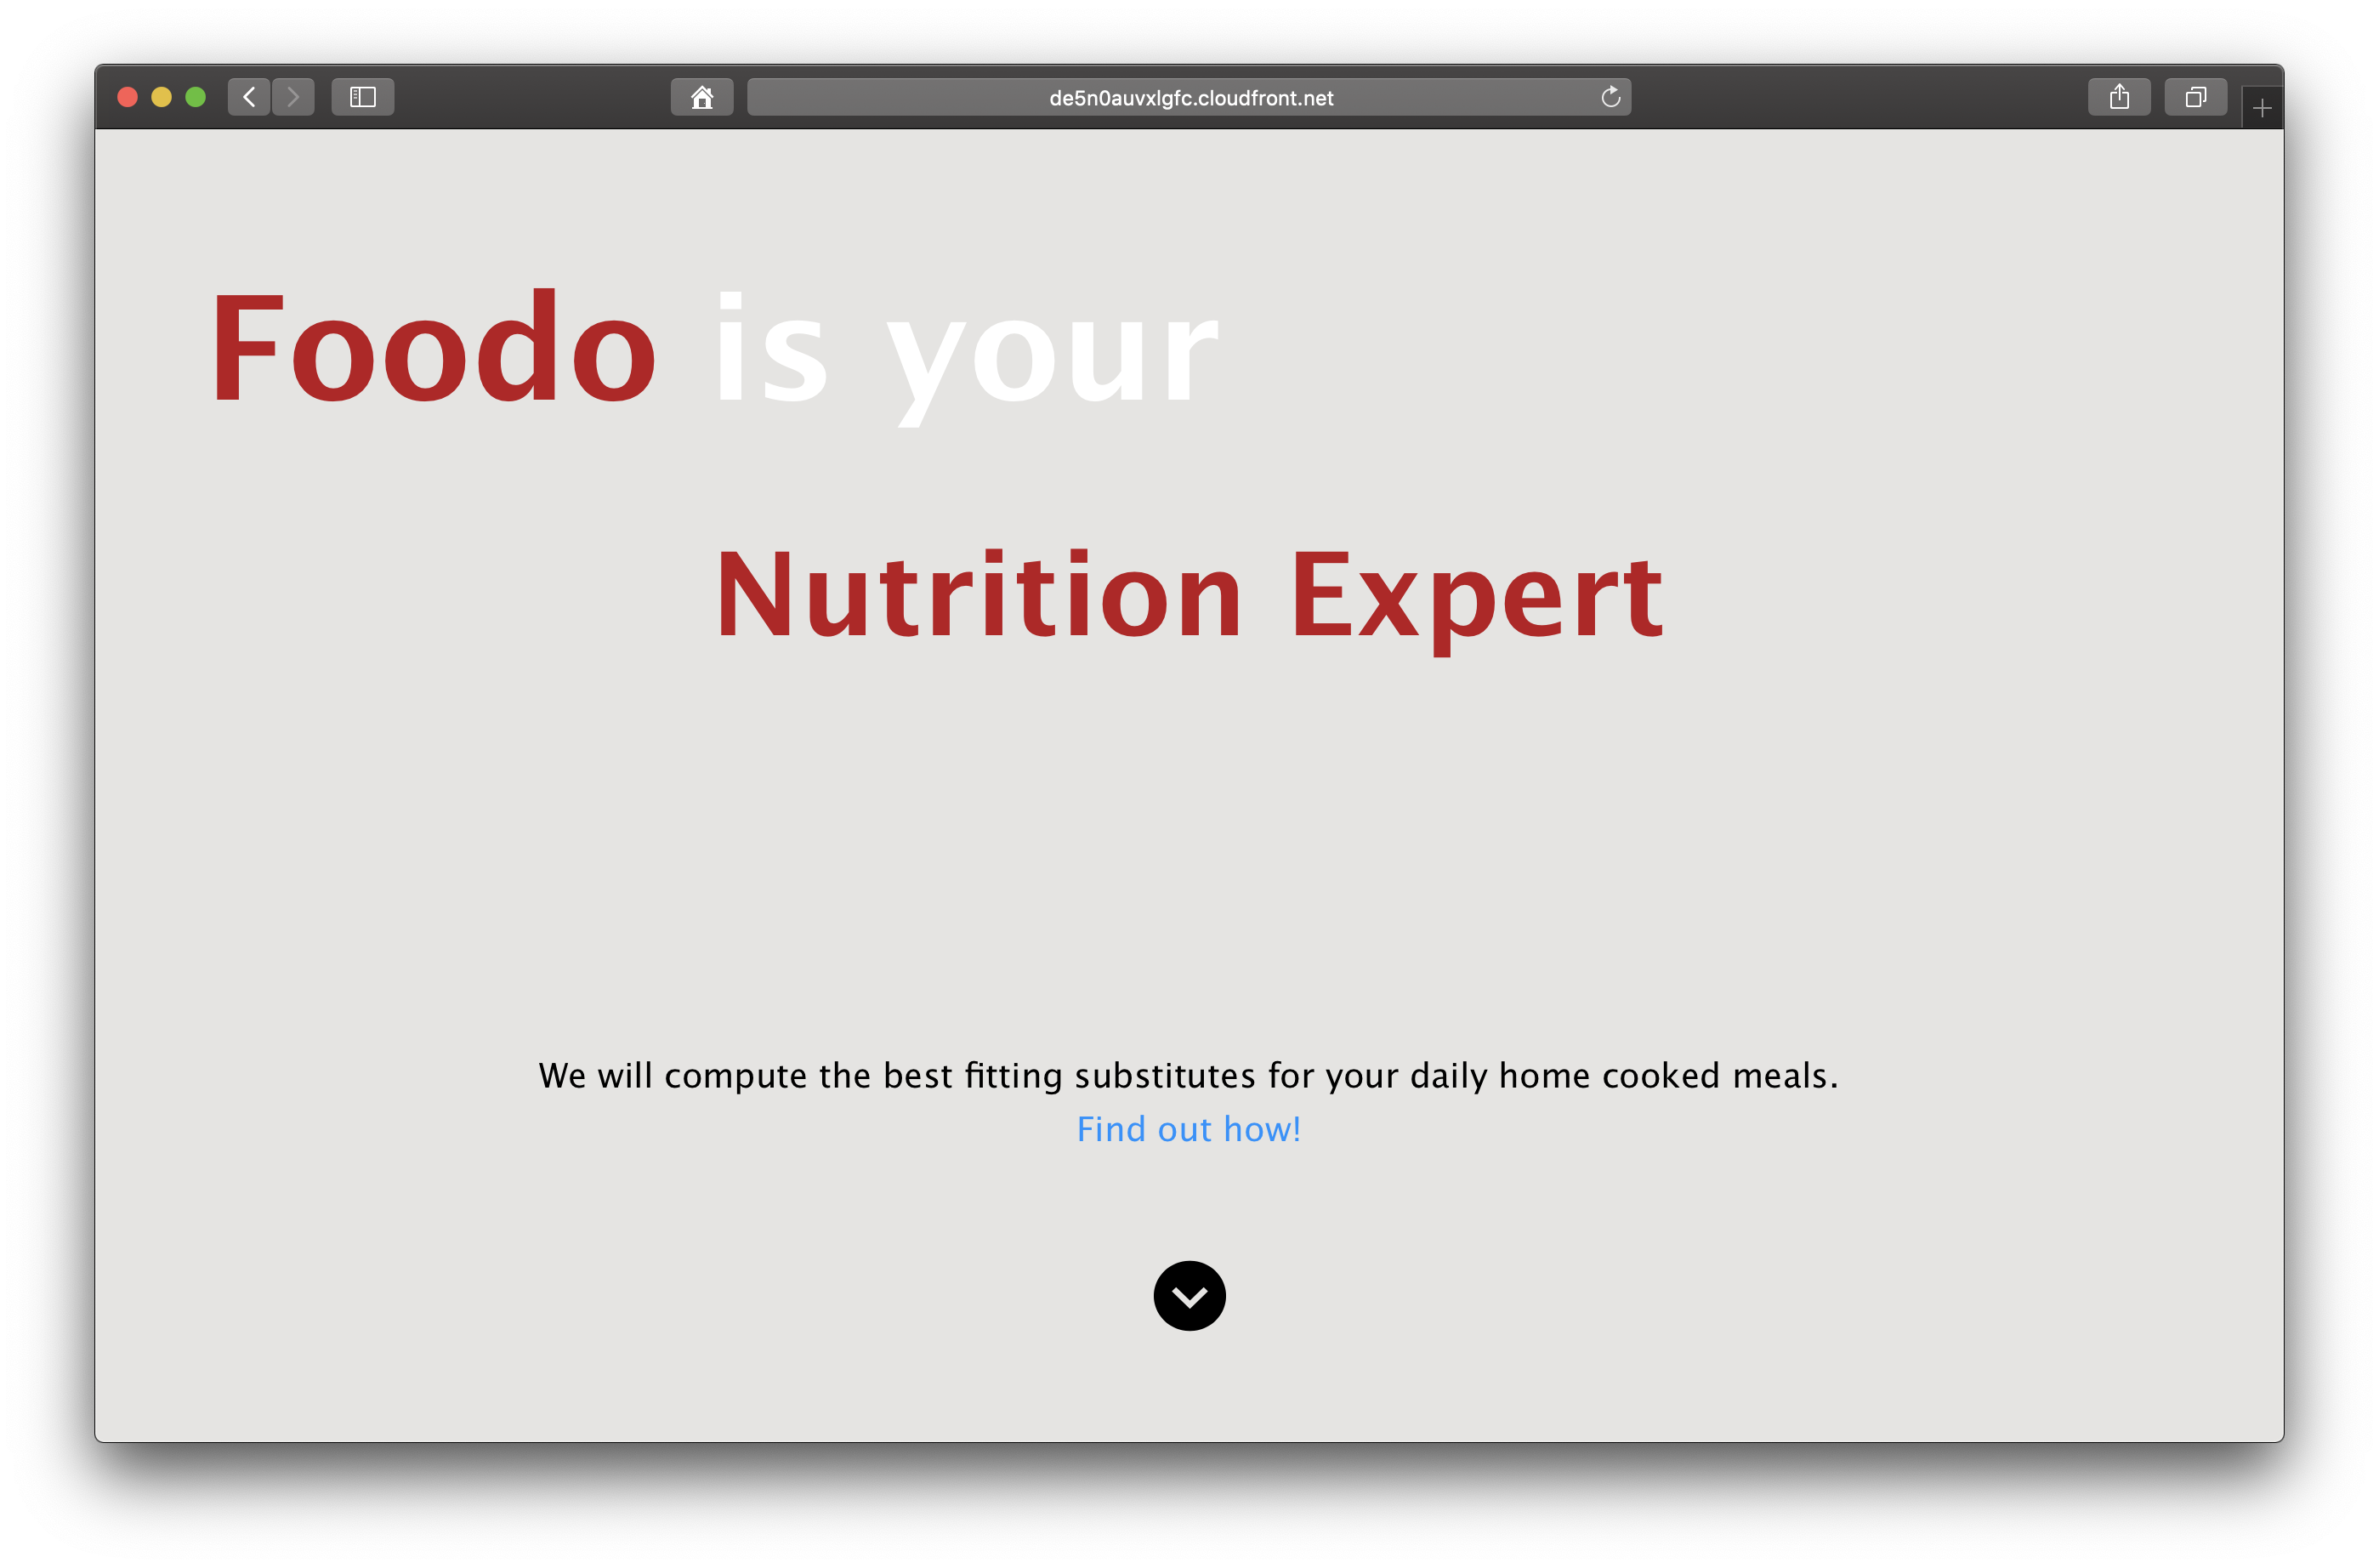
\includegraphics[scale=0.146]{Ressourcen/img/screenshots/About2.png}\hfill
		\includegraphics[scale=0.15]{Ressourcen/img/screenshots/screenshotB.png}\hfill
		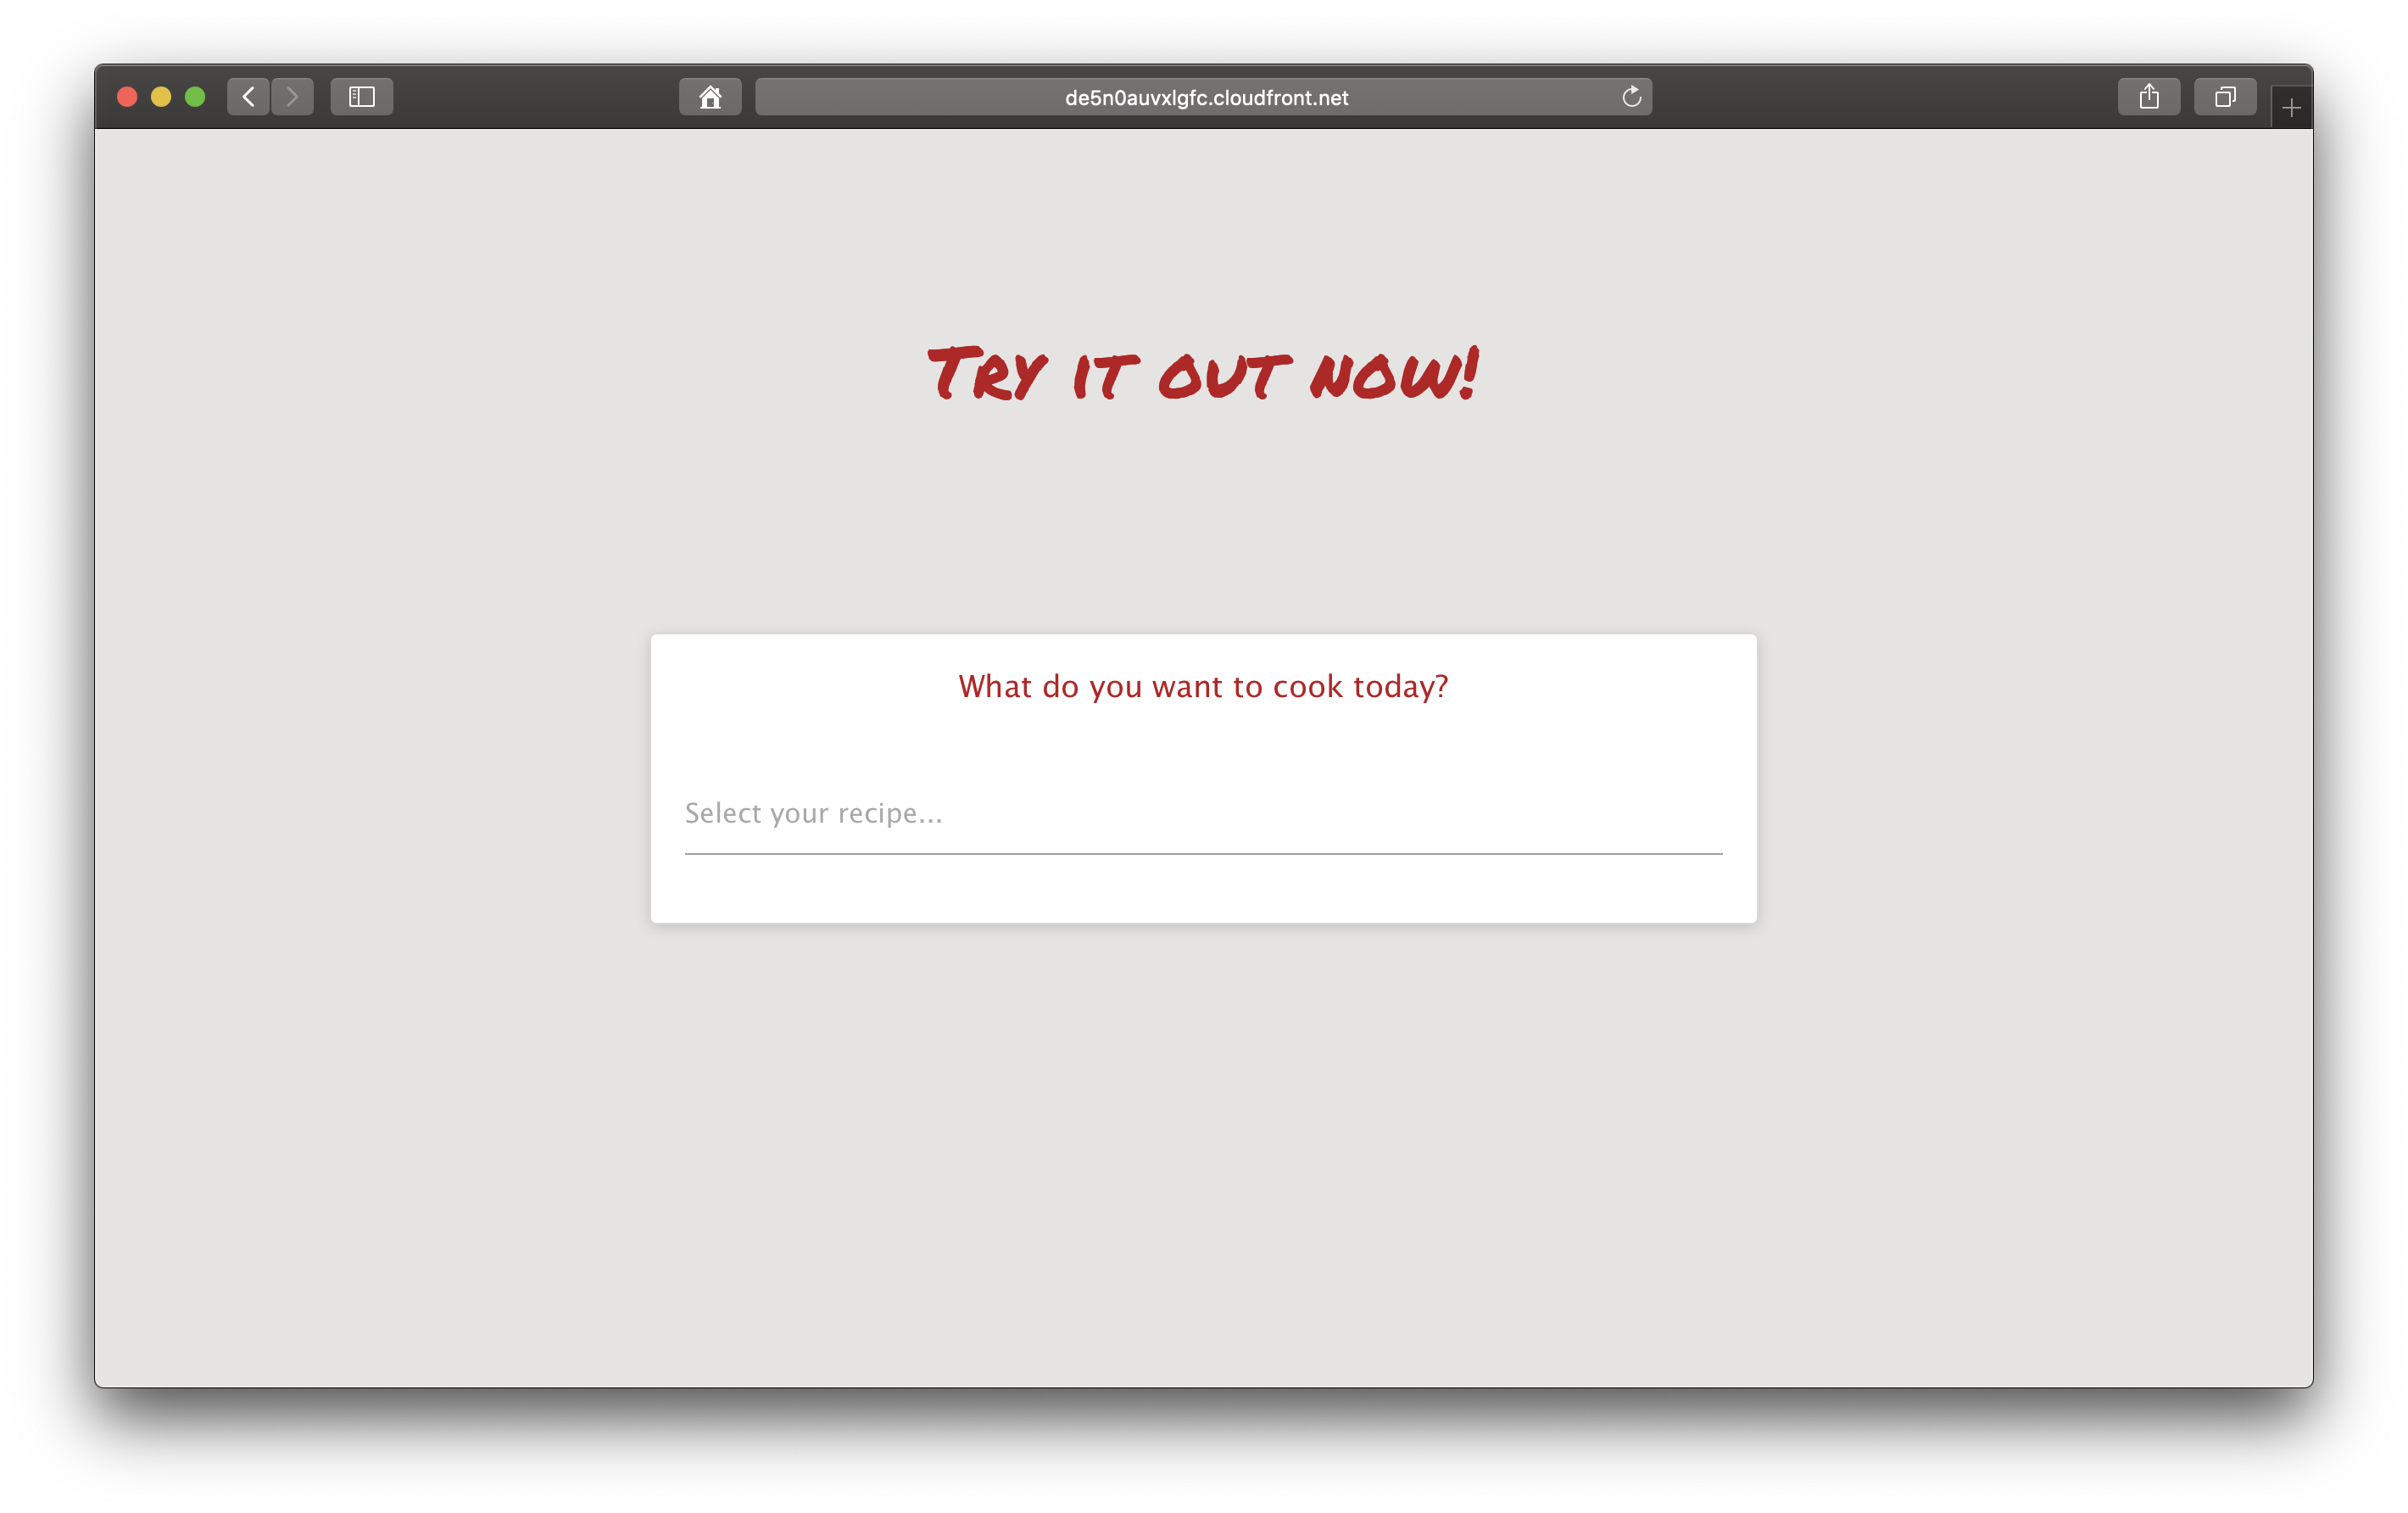
\includegraphics[scale=0.14]{Ressourcen/img/screenshots/screenshotC.png}
		\vspace{-1em}
		\caption{About-Us}
		\label{fig:aboutus}
	\end{center}
\end{figure}
\vspace{-3em}
Initially, a page visitor starts on our \texttt{About-Us} page which is also accessible by clicking on the \texttt{About-Us} index tab in the navigation menu. This page is separated into four subpages and mainly serves the purpose of informing the user about Foodo's services. If a user decides to give Foodo a try by either clicking on the \texttt{Get Started} button on the first subpage or by selecting a recipe he wants to cook on the last subpage (see figure \ref{fig:aboutus}), he will be forwarded to our \texttt{Login/Registration-Page} (see next section).
\subsection*{Login/Registration}
\vspace{0.5em}
\begin{figure}[H]
	\captionsetup{justification=centering}
	\begin{center}
		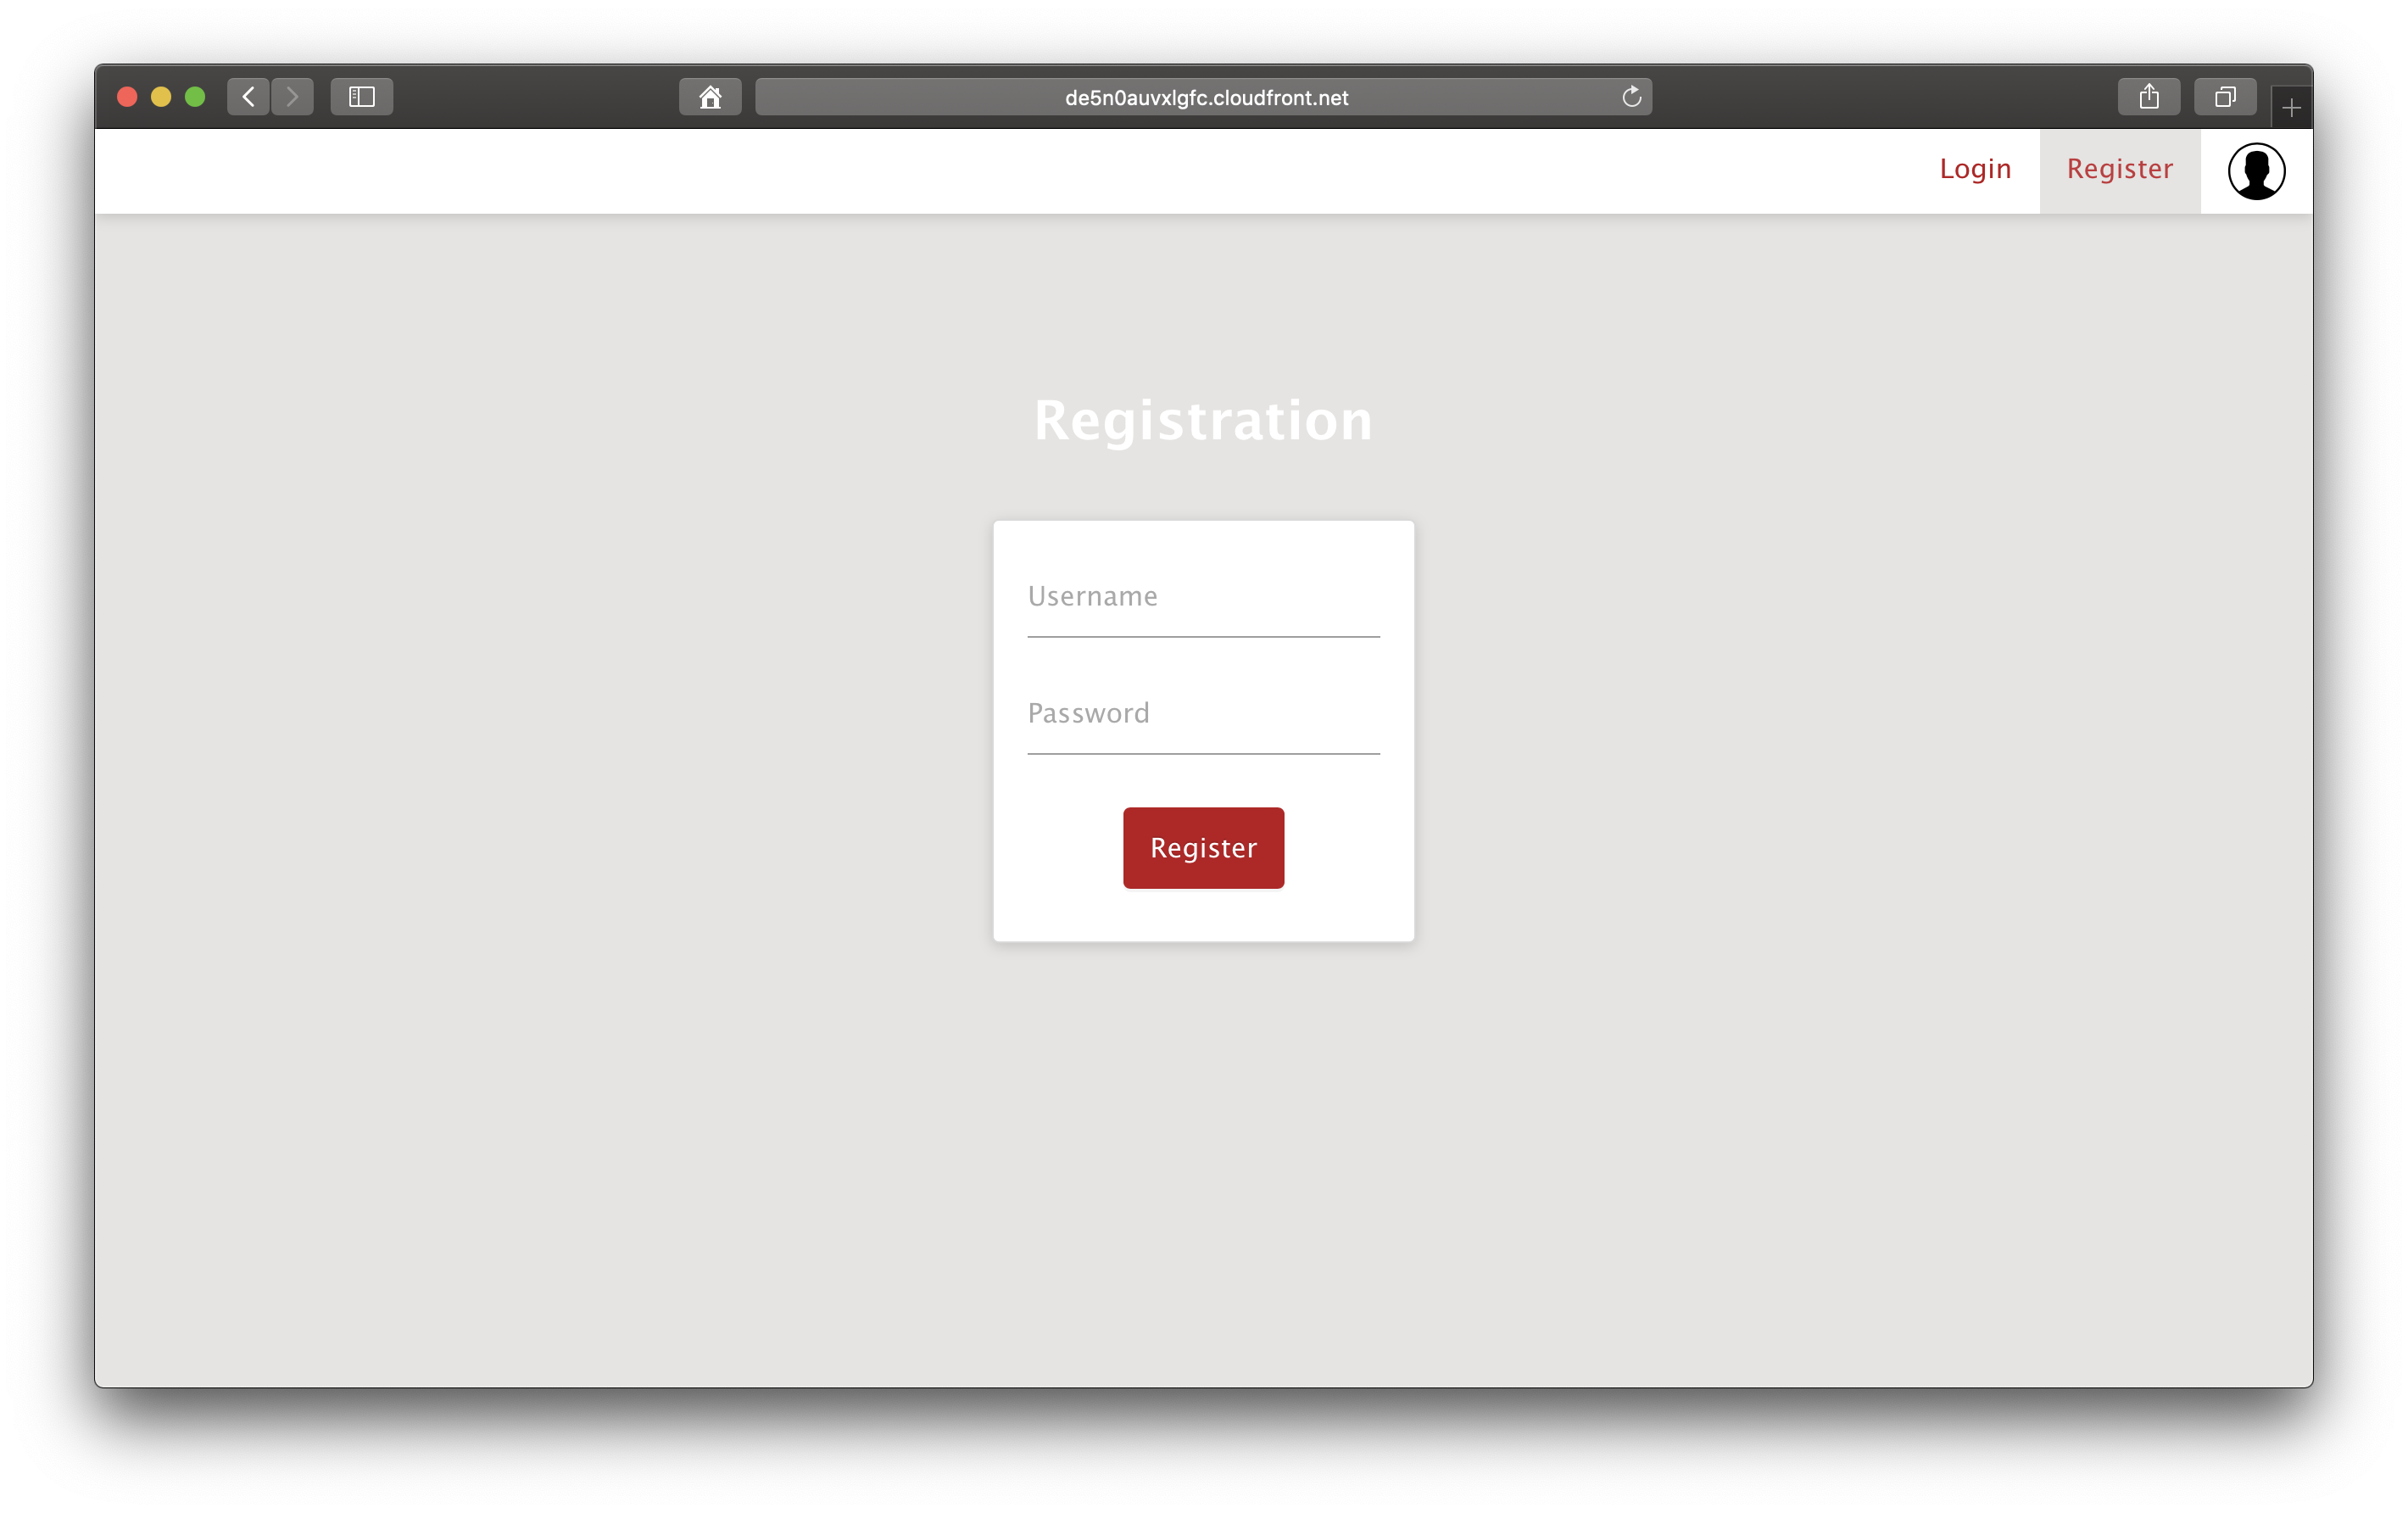
\includegraphics[scale=0.23]{Ressourcen/img/screenshots/screenshotD.png}
		\vspace{-2em}
		\caption{Registration}
		\label{fig:registration}
	\end{center}
\end{figure}
Before a user can use Foodo’s services, he first needs to create an account. Therefore, the user will always be redirected to the \texttt{Login/Registration-Page} (see figure \ref{fig:registration}) when the user tries to call a service URL or clicks the mentioned button or recipe selector in the previous section (\texttt{About-Us page}). By inserting an individual username, which has not been taken already, and a hopefully secure password, the user can create a new account. The user also has the option to login with an already registered account by clicking on \texttt{Login} in the right upper corner and inserting his previously created credentials in the following form.
\subsection*{Navigation bar}
\vspace{0.5em}
\begin{figure}[H]
	\captionsetup{justification=centering}
	\begin{center}
		\includegraphics[scale=0.4]{Ressourcen/img/screenshots/screenshotE.png}
		\vspace{-3em}
		\caption{Navbar}
		\label{fig:navbar}
	\end{center}
\end{figure}
\vspace{-3em}
In the previous sections, there was no navigation bar at the top of the screen, as one could see in the figures. This was mainly a aesthetic design decision but also hides unavailable options for non-authenticated users. Now, after a user has logged into his account, the navigation bar is visible, shown in figure \ref{fig:navbar}. By clicking on the profile icon in the upper right corner, a menu panel will be shown with additional navigation options for the user. Overall, he has the following navigation options:
\begin{itemize}
\item \textbf{Home}: The main page of Foodo, described in the next section
\item \textbf{My Profile}: The user's settings and preferences regarding food items and nutrition; described in section Profile Page.
\item \textbf{Statistics}: The user's improvements depicted with graphics and values; described in section \texttt{Statistics}.
\item \textbf{Preferences}: This will open another small menu panel with two submenus. Clicking on \texttt{Languages} will again open another small menu panel, where the user can choose between the offered languages (currently only English and German). Clicking on \texttt{Password} will direct the user to a form, where he can insert his new password.
\item \textbf{About}: This will direct the user to the \texttt{About-Page} again.
\item \textbf{Logout}: This is quite self explanatory and will logout the user from his current account.
\end{itemize}
\subsection*{Home page}
\vspace{0.5em}
\begin{figure}[H]
	\captionsetup{justification=centering}
	\begin{center}
		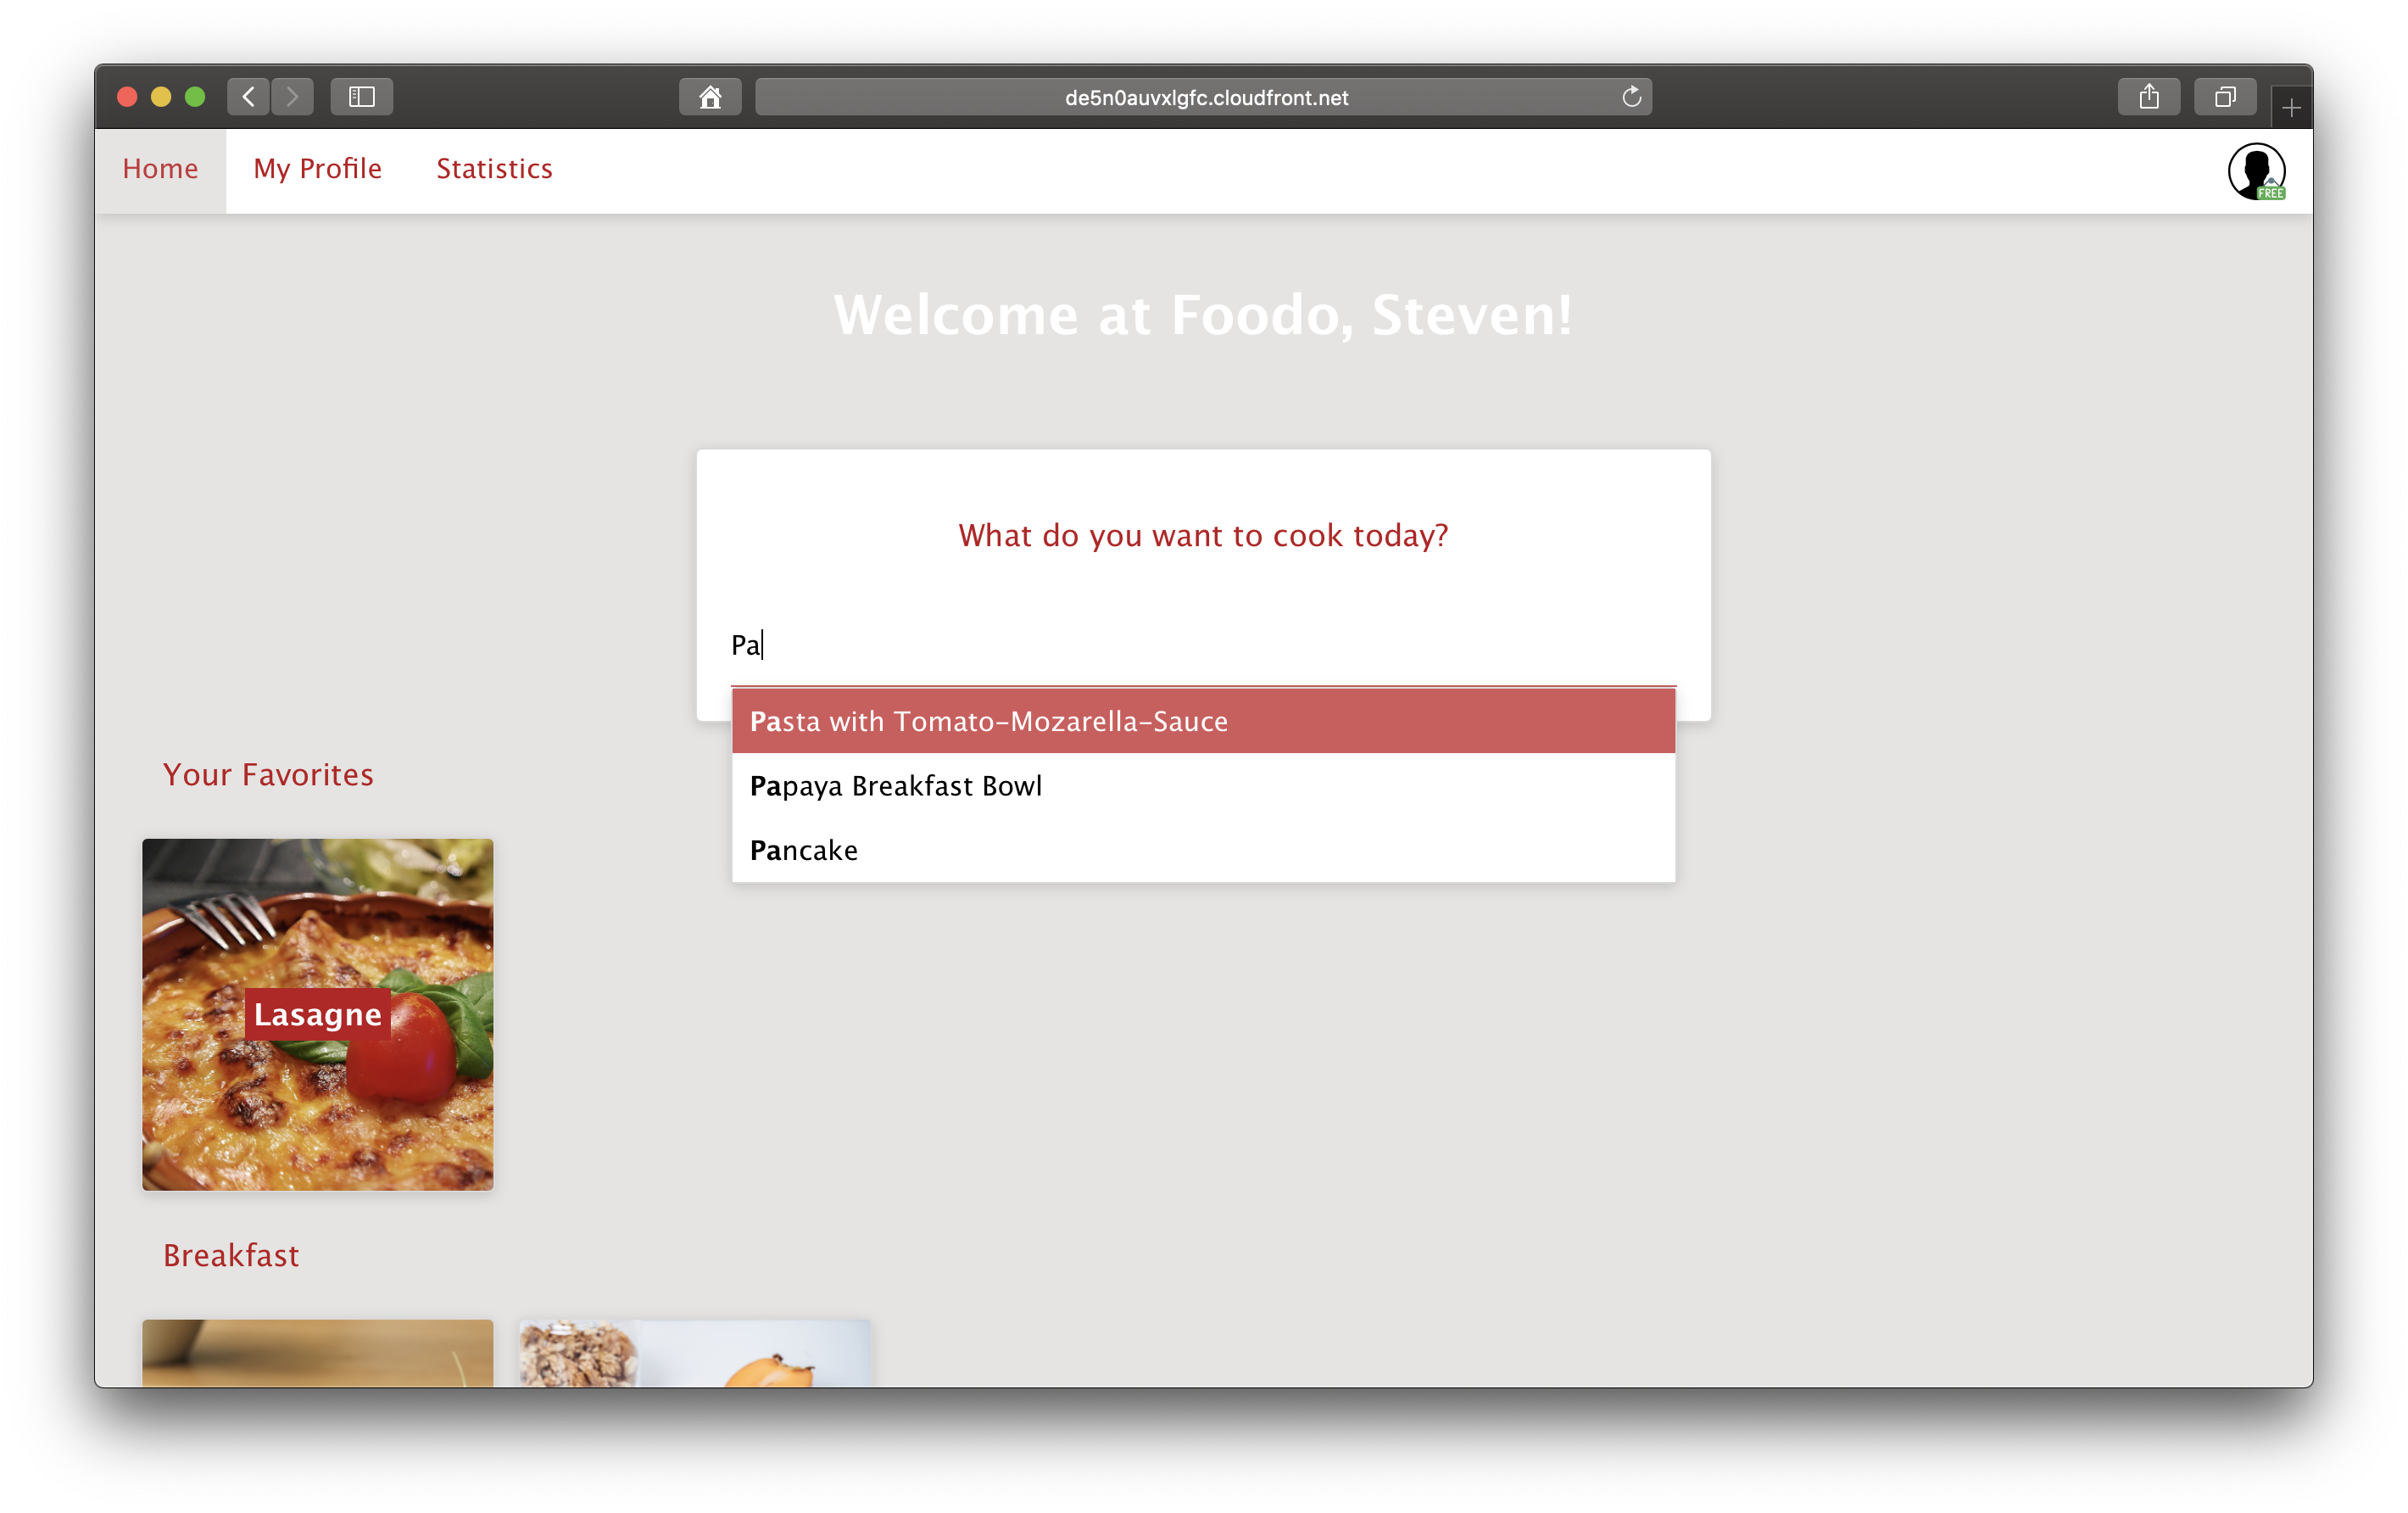
\includegraphics[scale=0.30]{Ressourcen/img/screenshots/screenshotF.png}
		\vspace{-3em}
		\caption{Home page recipe selector }
		\label{fig:recipeSelector}
	\end{center}
\end{figure}
\vspace{-2em}
\begin{figure}[H]
	\captionsetup{justification=centering}
	\begin{center}
		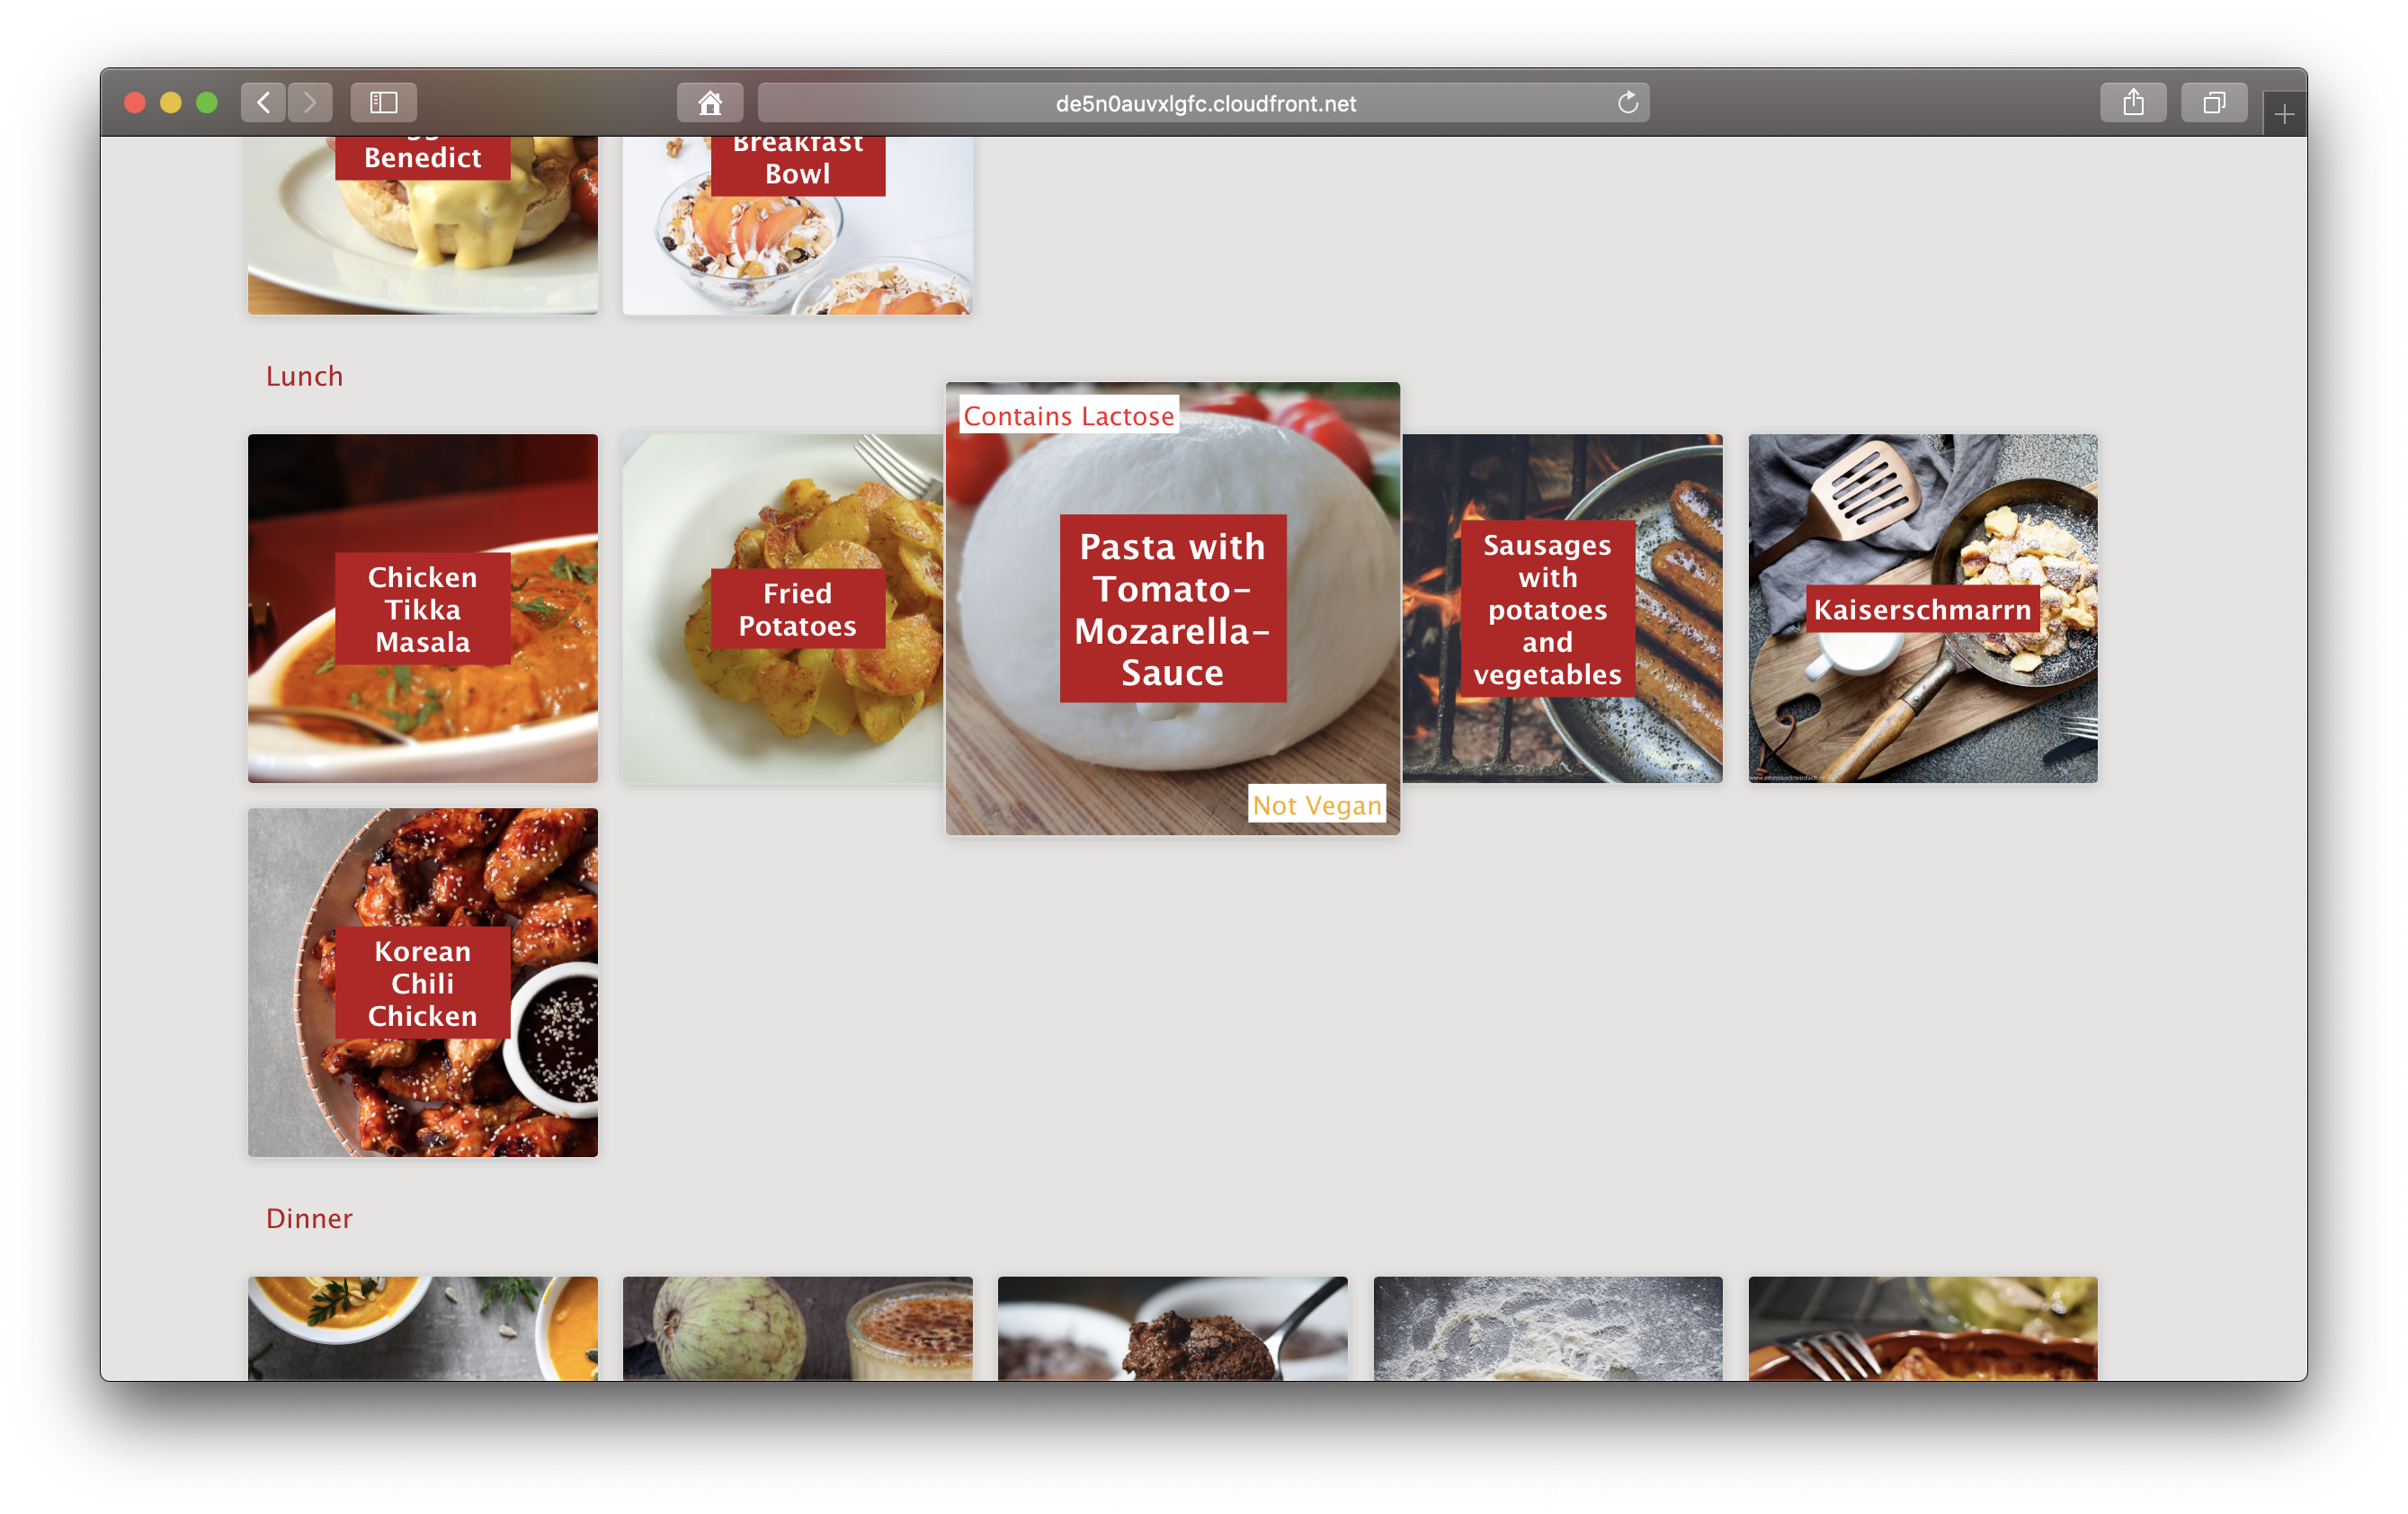
\includegraphics[scale=0.30]{Ressourcen/img/screenshots/screenshotG.png}
		\vspace{-1em}
		\caption{Home page recipe tiles}
		\label{fig:recipeTiles}
	\end{center}
\end{figure}
\vspace{-2em}
This is the main page of our application where the user can browse through a variety of recipes. Browsing the available recipes and eventually choosing one recipe to cook can be achieved either by clicking on the \texttt{'Select your recipe…'} input field and selecting a recipe out of the appearing list (see figure \ref{fig:recipeSelector}) or by scrolling through the displayed recipe boxes below (see figure \ref{fig:recipeTiles}). The different recipe boxes have been designed to appear visual appealing by showing preview pictures of the dishes. Furthermore, each box shows useful personalized information about supported lifestyle and allergies on hover. To improve the user experience, the boxes are also categorized into four standard groups and two categories that match the user's lifestyle and allergies:
\begin{itemize}
\item Your Favorites
\item Breakfast
\item Lunch
\item Dinner
\item Tolerated recipes (allergy-based)
\item Lifestyle (e.g. Vegan, Vegetarian)
\end{itemize}	
However, before the user can start the substitution process, it is advised to go to the personal preferences page and select at least a personal nutrition goal. This instruction is displayed in a yellow box, as shown in figure \ref{fig:profilesetting}.

\vspace{-1em}
\begin{figure}[H]
	\captionsetup{justification=centering}
	\centering
	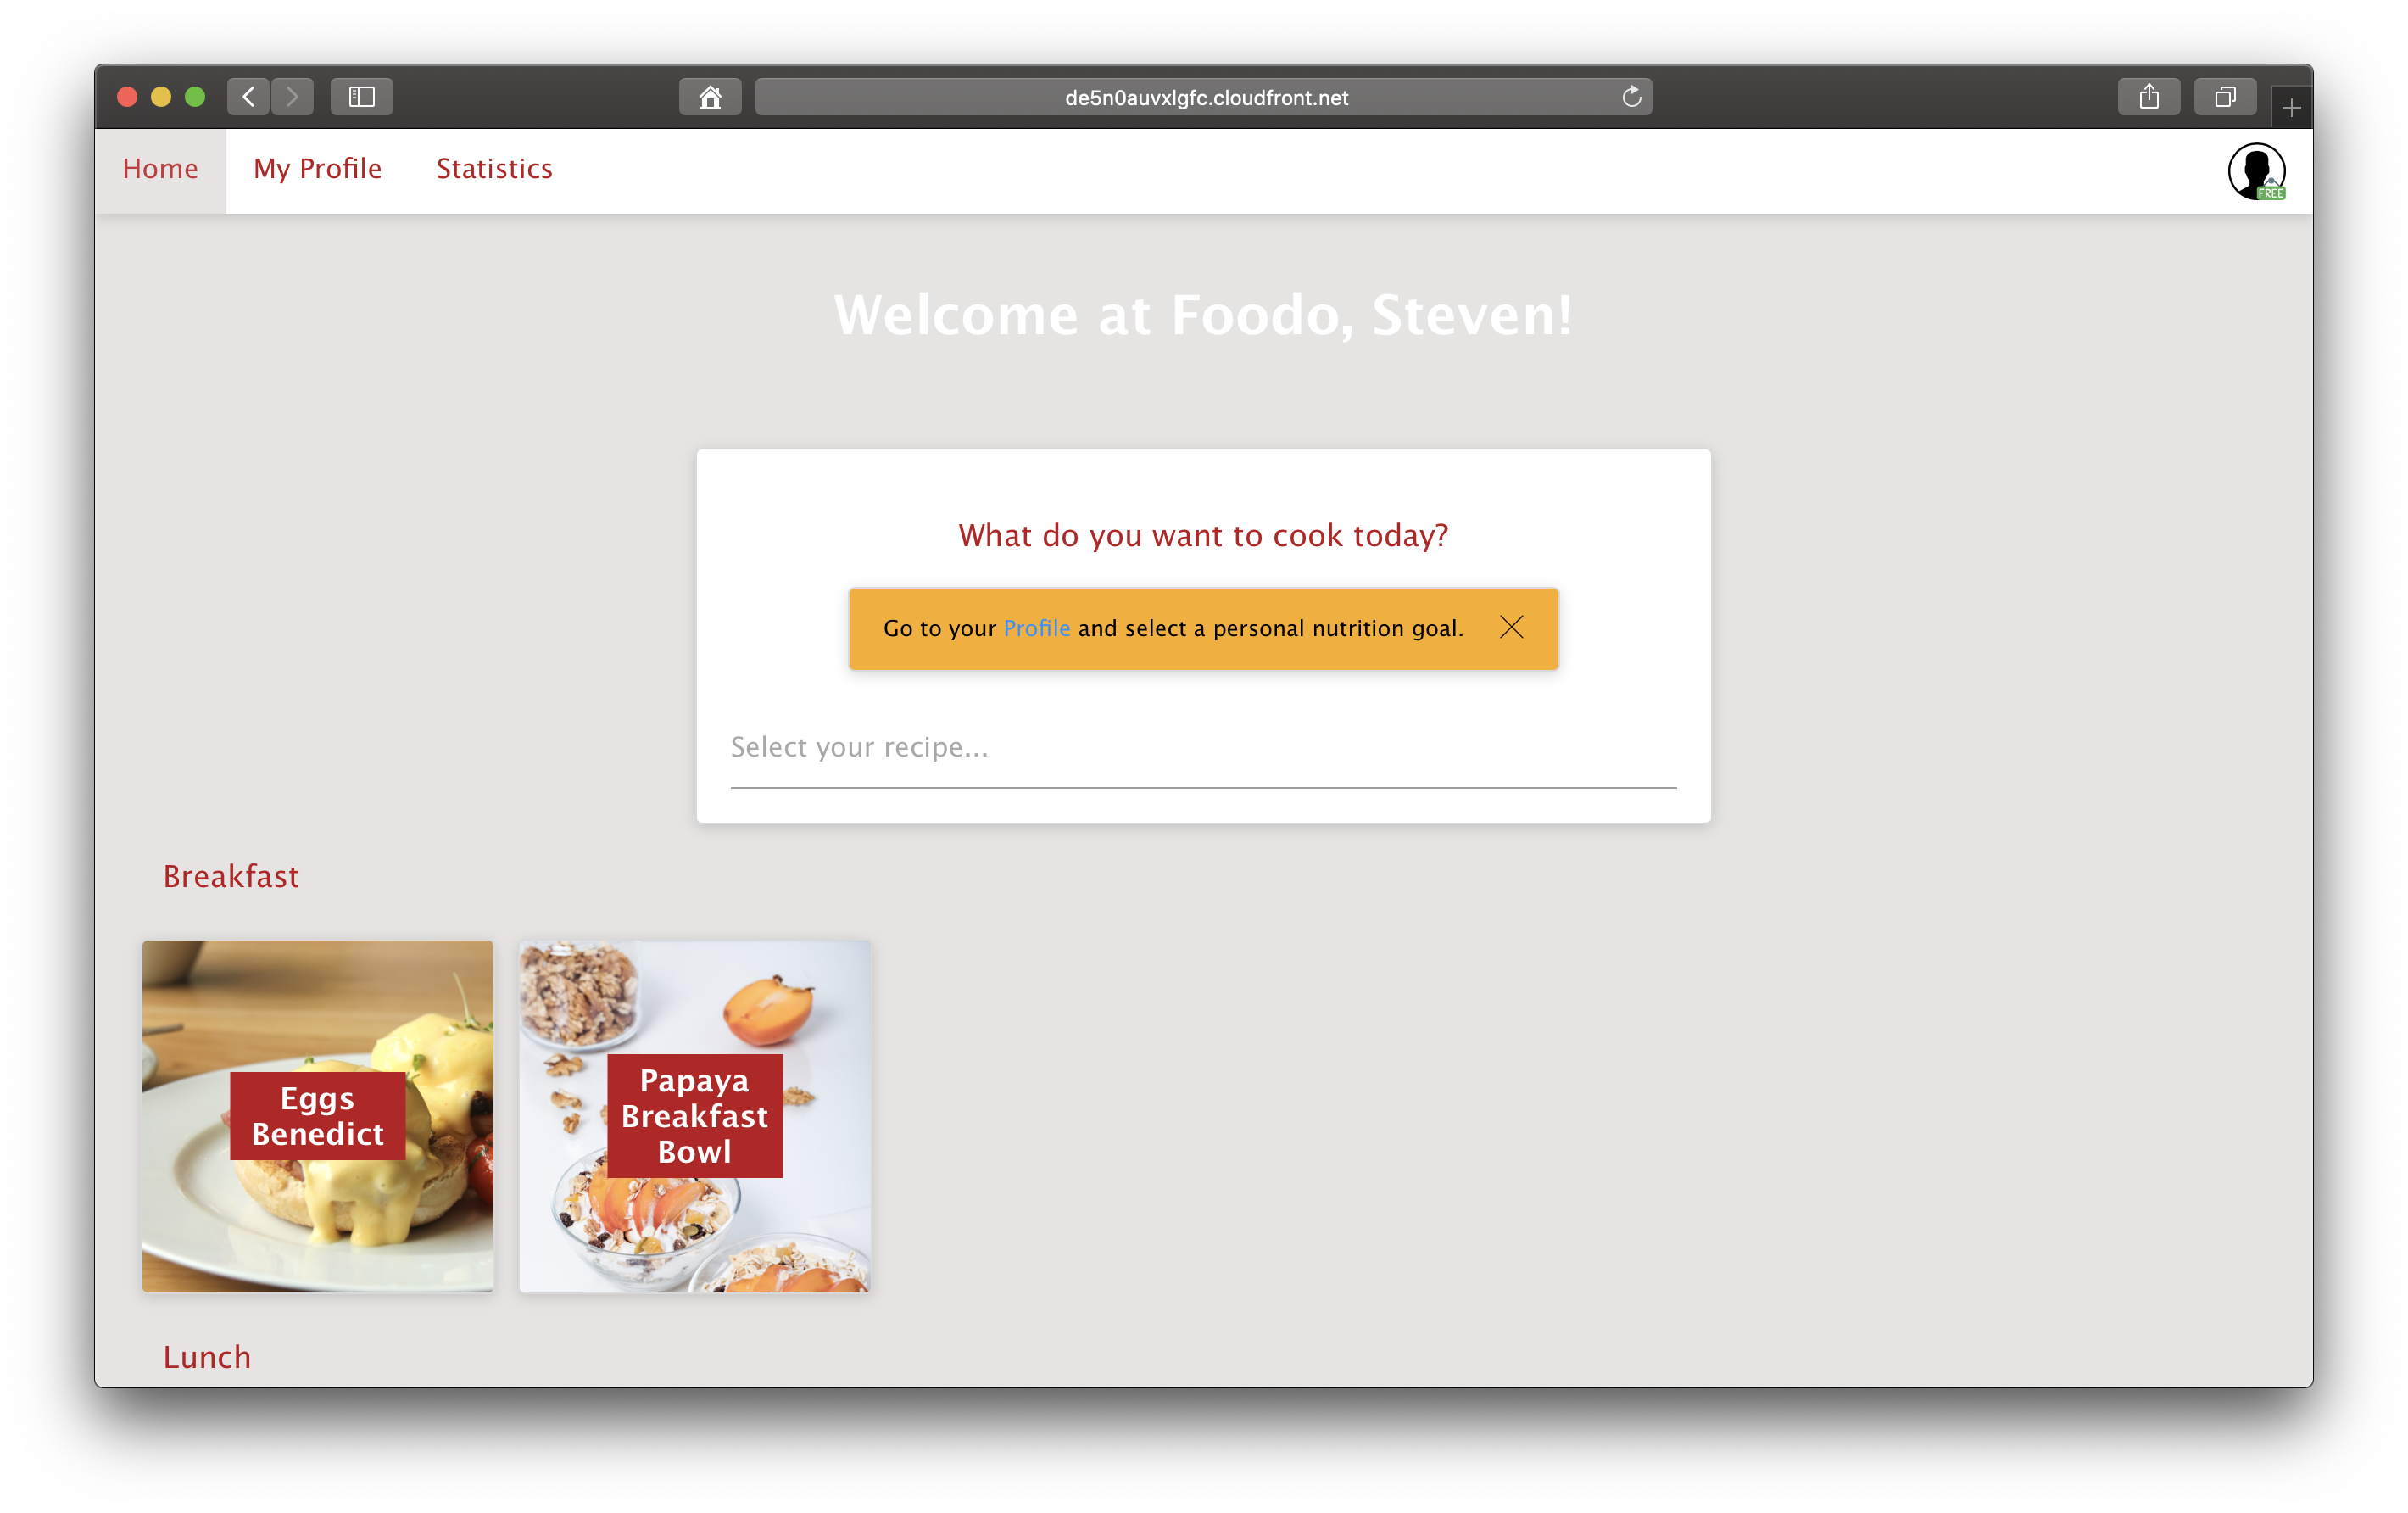
\includegraphics[scale=0.30]{Ressourcen/img/screenshots/screenshot41.png}
	\vspace{-3em}
	\caption{Profile settings for user}
	\label{fig:profilesetting}
\end{figure}

\subsection*{Recipe detail view}
\vspace{0.5em}
\begin{figure}[H]
	\captionsetup{justification=centering}
	\centering
		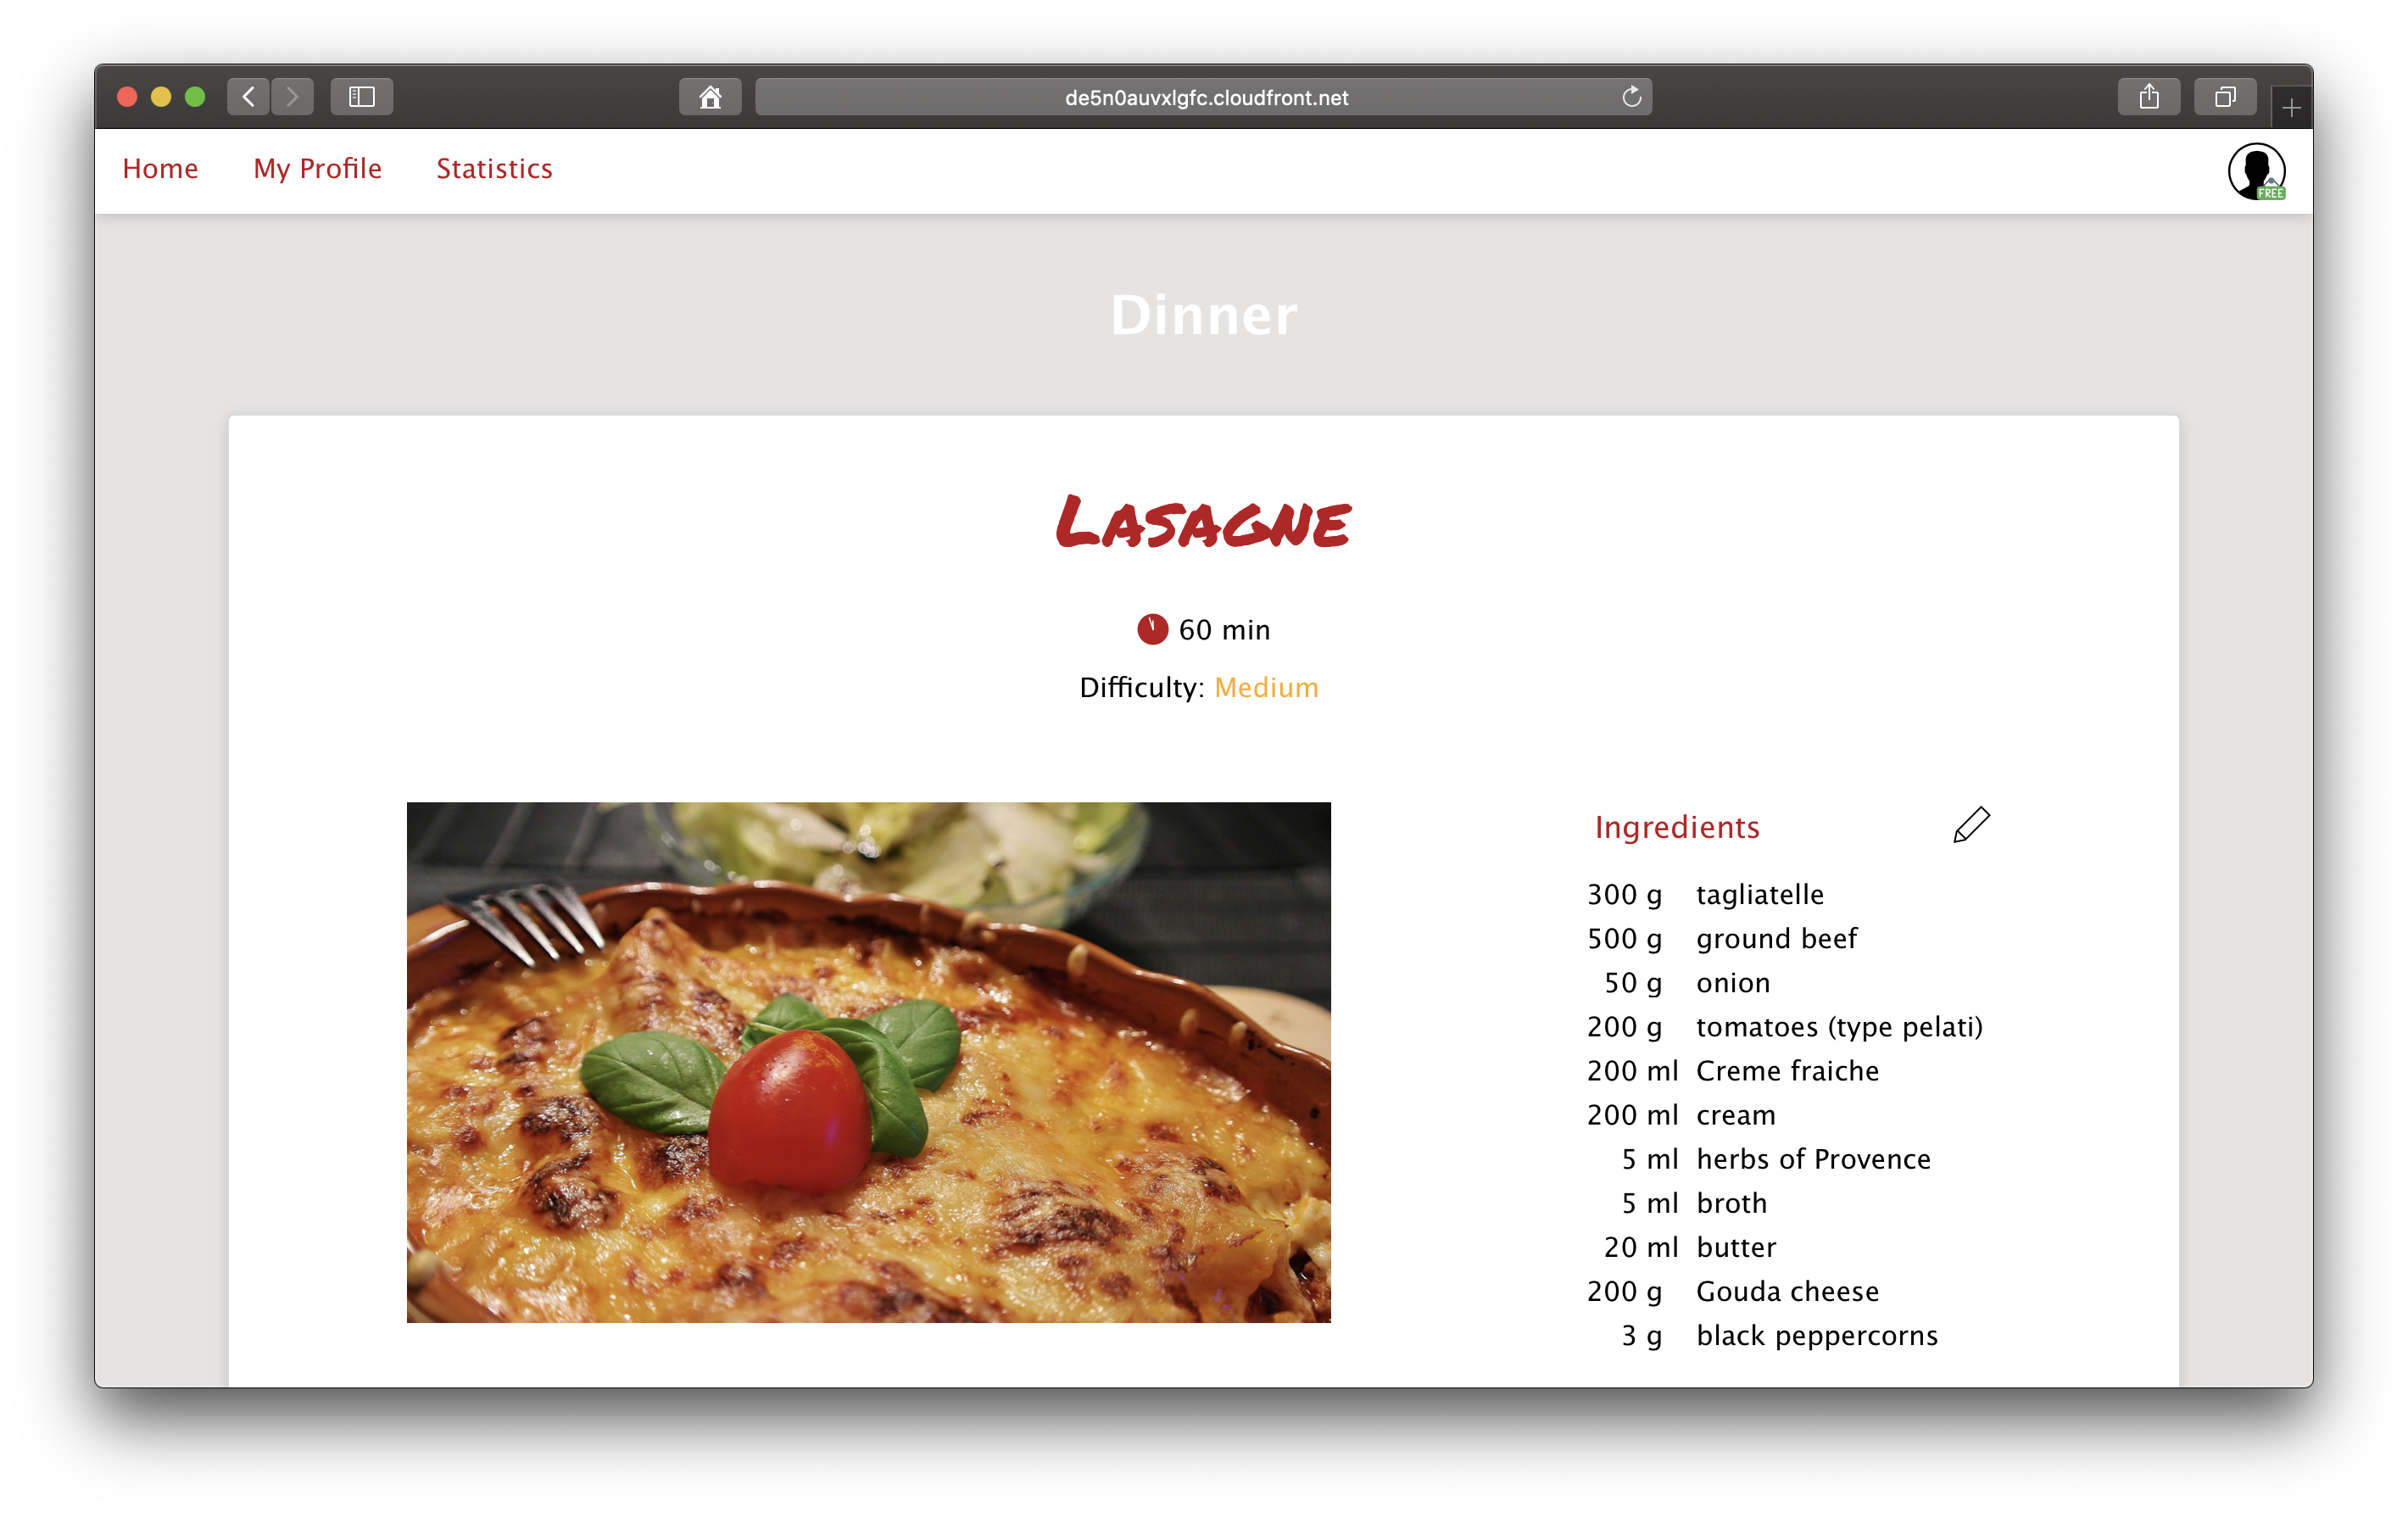
\includegraphics[scale=0.25]{Ressourcen/img/screenshots/screenshotH.png}
		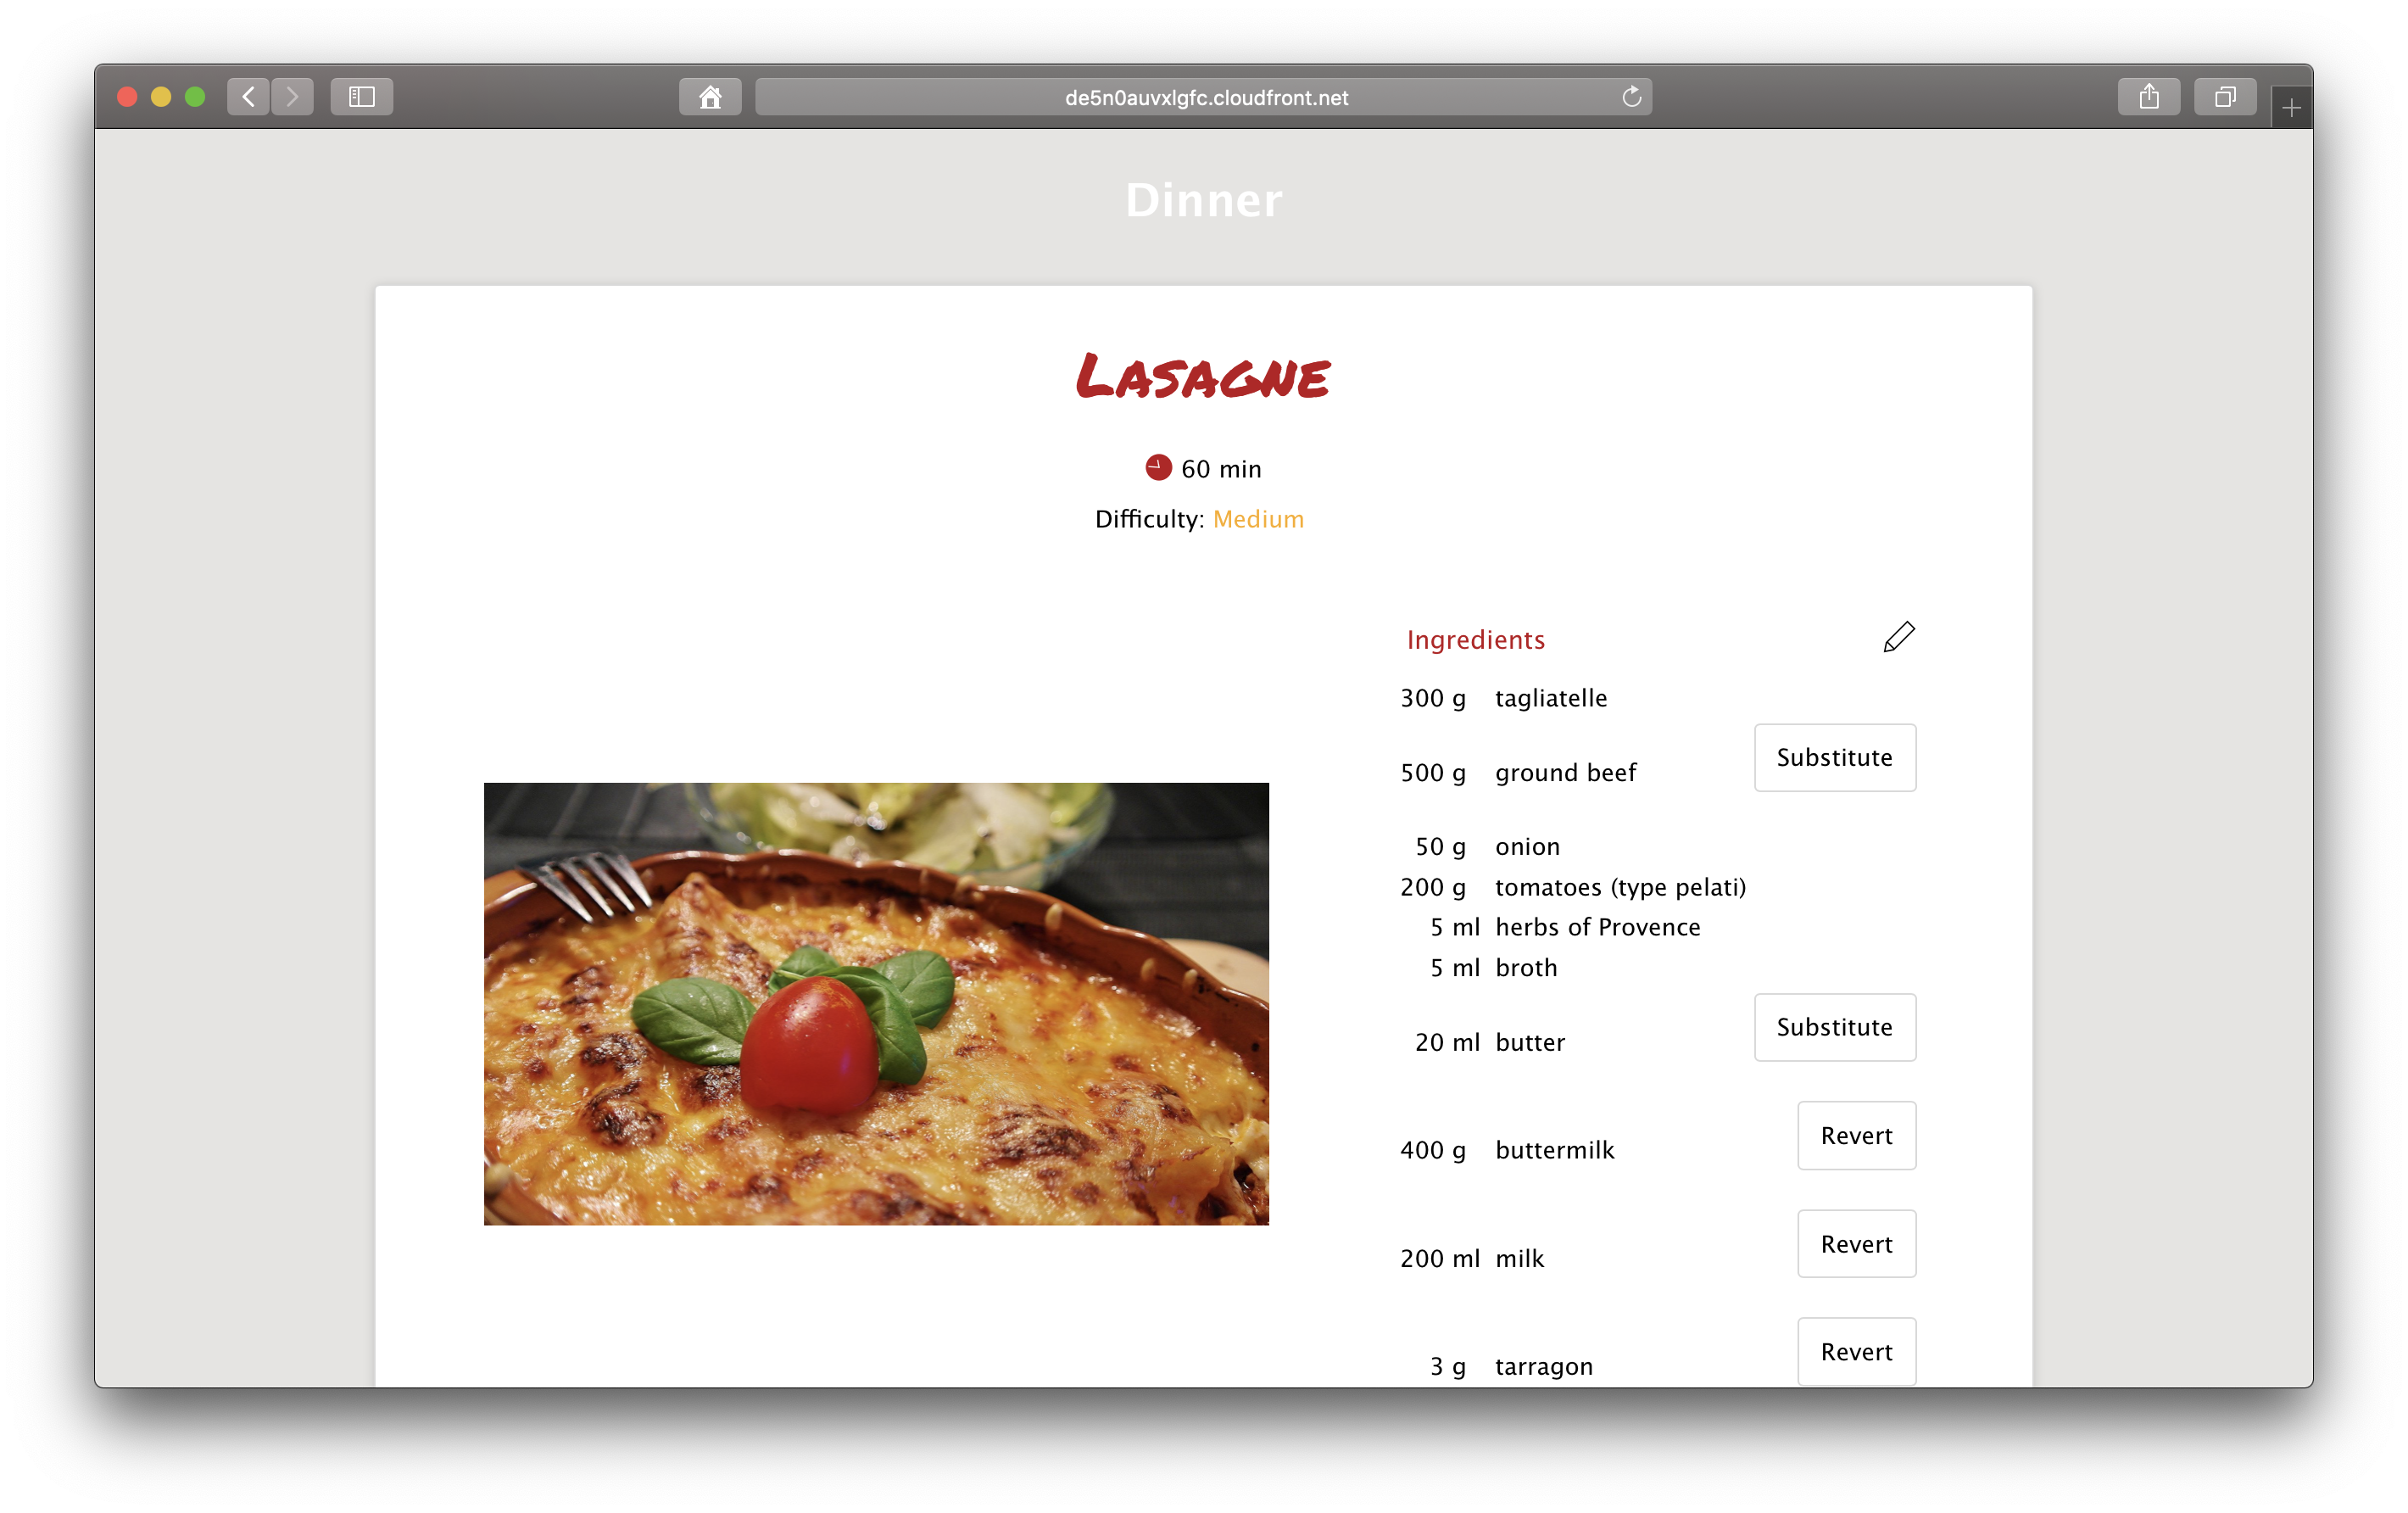
\includegraphics[scale=0.25]{Ressourcen/img/screenshots/screenshotI.png}
		\vspace{-1em}
		\caption{Recipe detail view without and with selected user goal}
		\label{fig:recipeDetail}
\end{figure}
\vspace{-2em}
The first part of the detailed recipe overview consists of a picture and a list of ingredients. Depending on whether the user already selected his personal goal, the user either sees the first or second view depicted in figure \ref{fig:recipeDetail}. For those ingredients where there exists a better substitute in our database based on the nutriscore, a \texttt{Substitute} button will be displayed. By clicking on it, the user can select a suitable substitute as shown in figure \ref{fig:substitute}. (You can find more information regarding the substitution algorithm in chapter \emph{\ref{algorithm}  Algorithm}). In the newly opened window the user can see the current NutriScore and possible alternatives for the selected ingredients together with their individual NutriScore. If the user already substituted an ingredient and wishes to revert the substitution, this can be achieveed by clicking on the meanwhile displayed \texttt{Revert} button next to the substitute. 
There is also the option to personalize the recipe by clicking on the pencil icon on top of the ingredients list. This will open the window shown in figure \ref{fig:personalisation} where the user can add or remove current ingredients.

\vspace{-1em}
\begin{figure}[H]
	\captionsetup{justification=centering}
	\begin{center}
		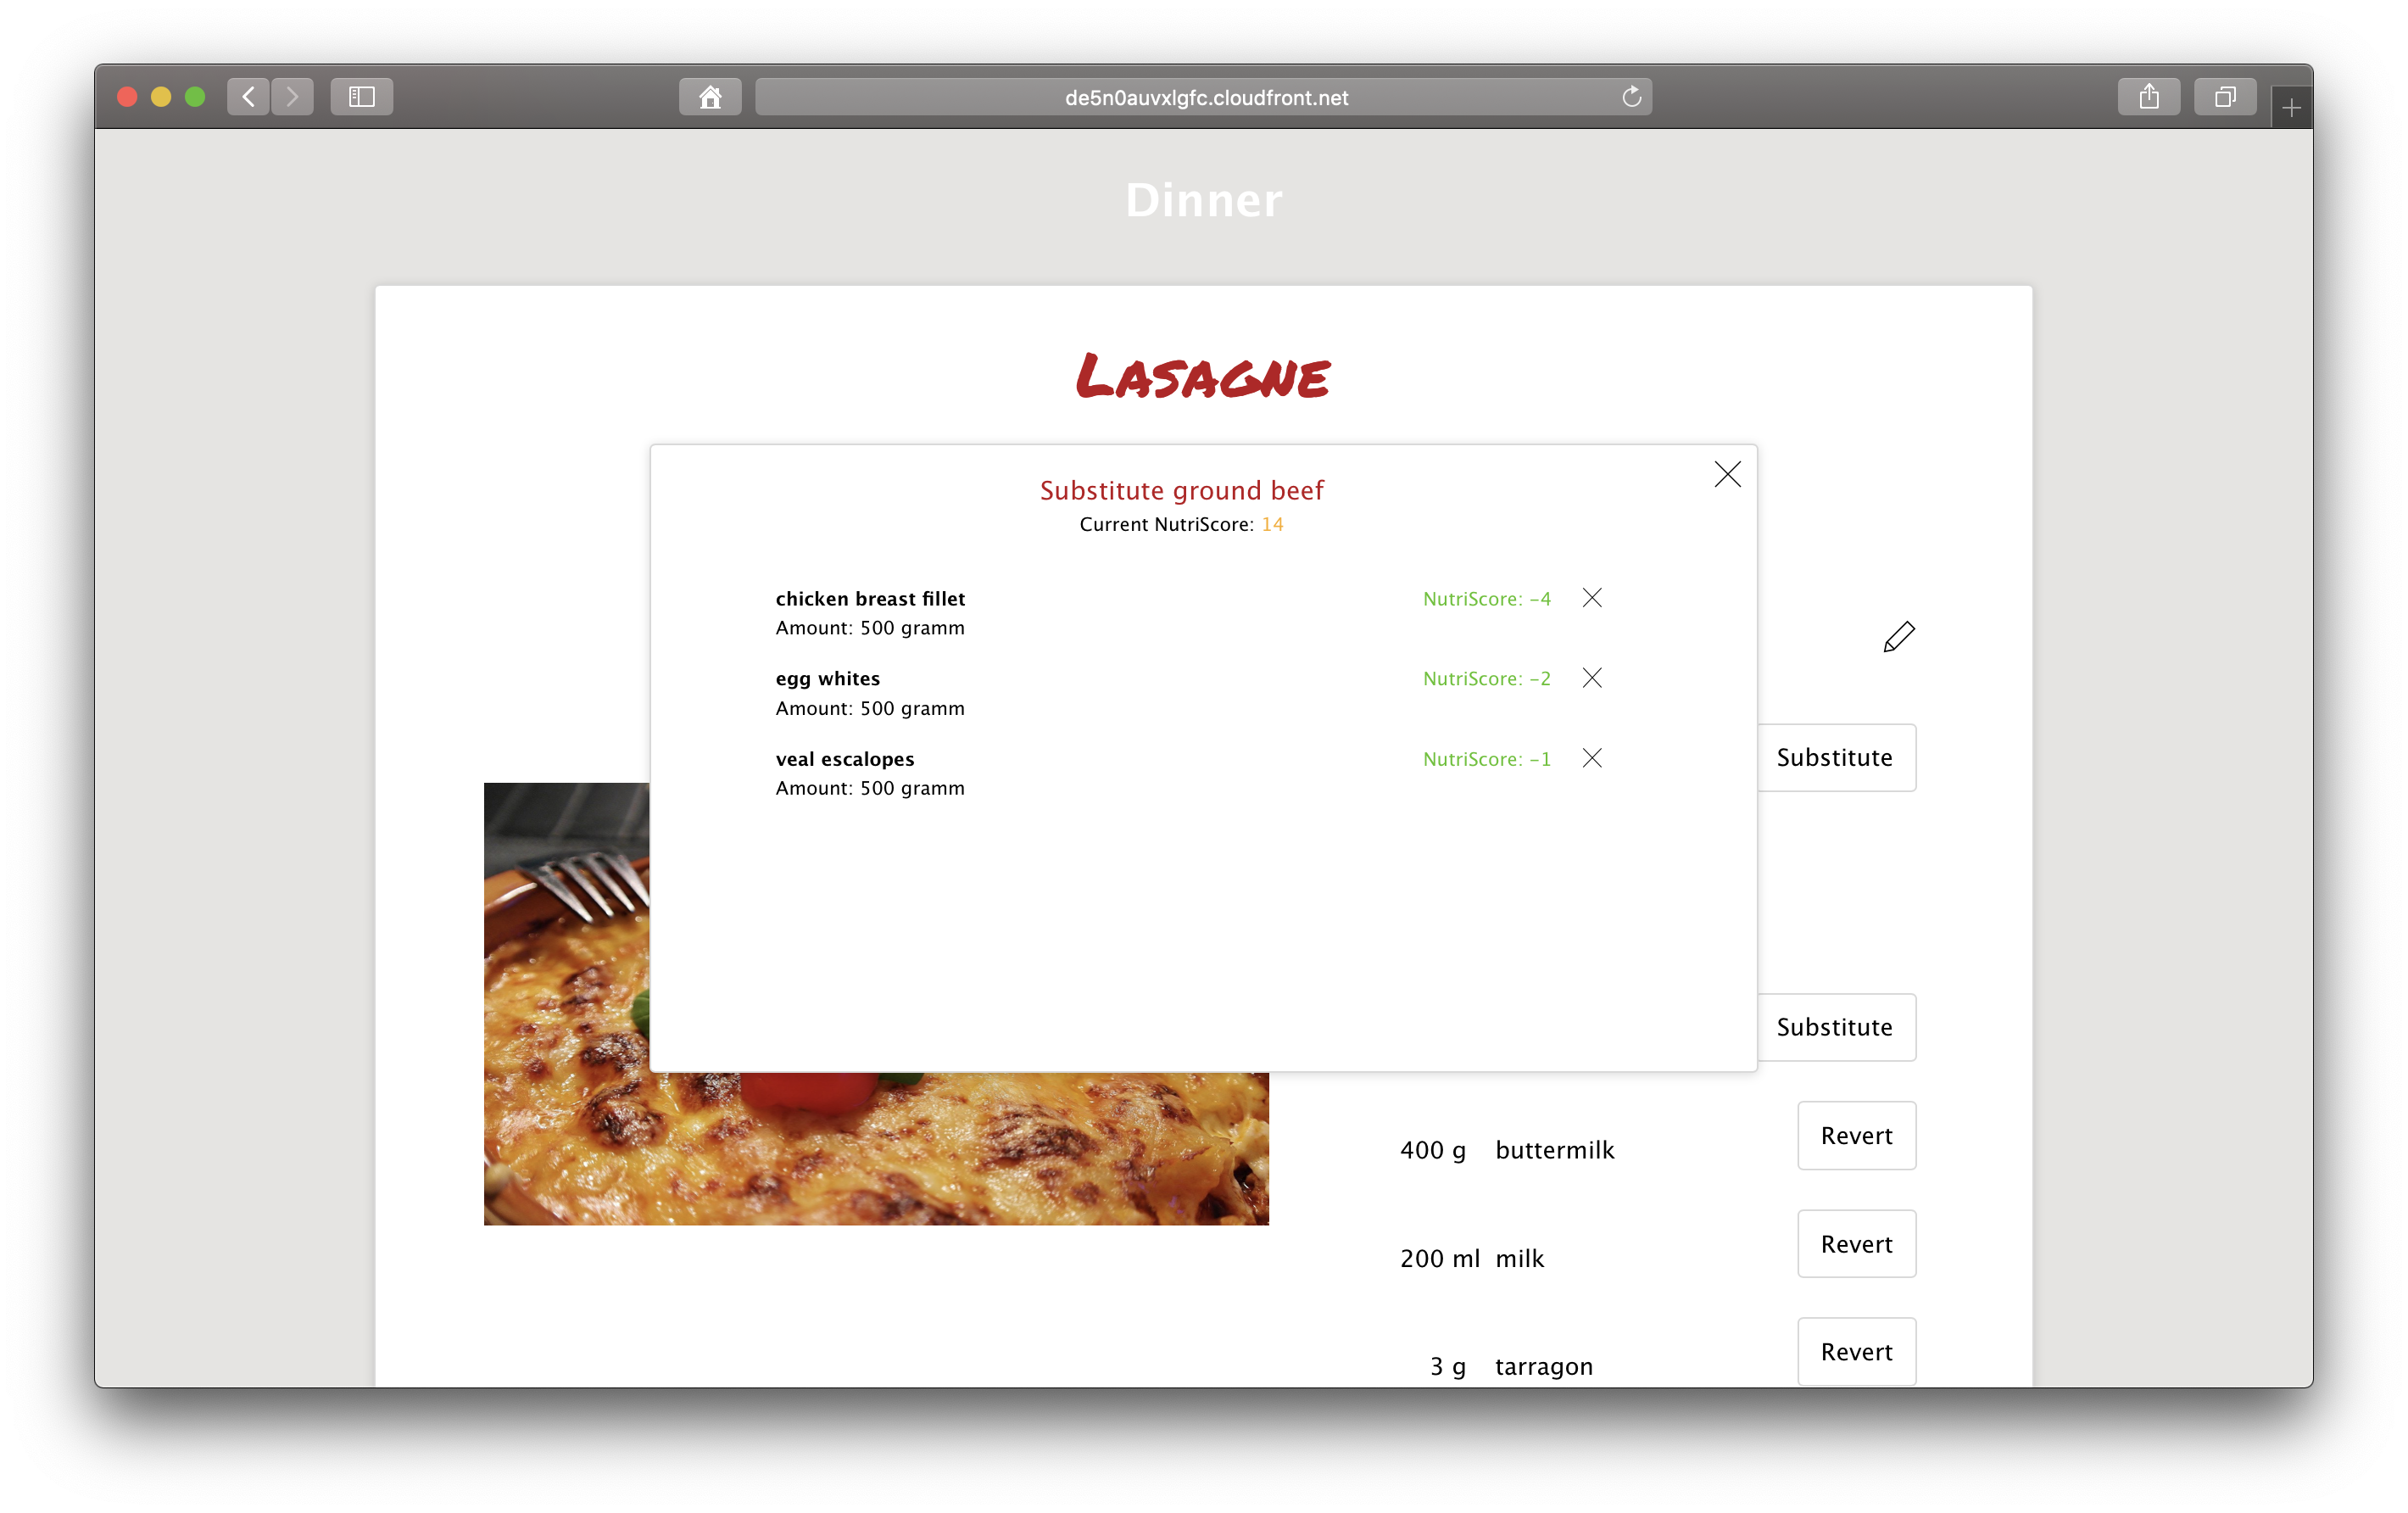
\includegraphics[scale=0.28]{Ressourcen/img/screenshots/screenshotJ.png}
		\vspace{-3em}
		\caption{Potential substitutes for beef}
		\label{fig:substitute}
	\end{center}
\end{figure}

\vspace{-2em}
\begin{figure}[H]
	\captionsetup{justification=centering}
	\begin{center}
		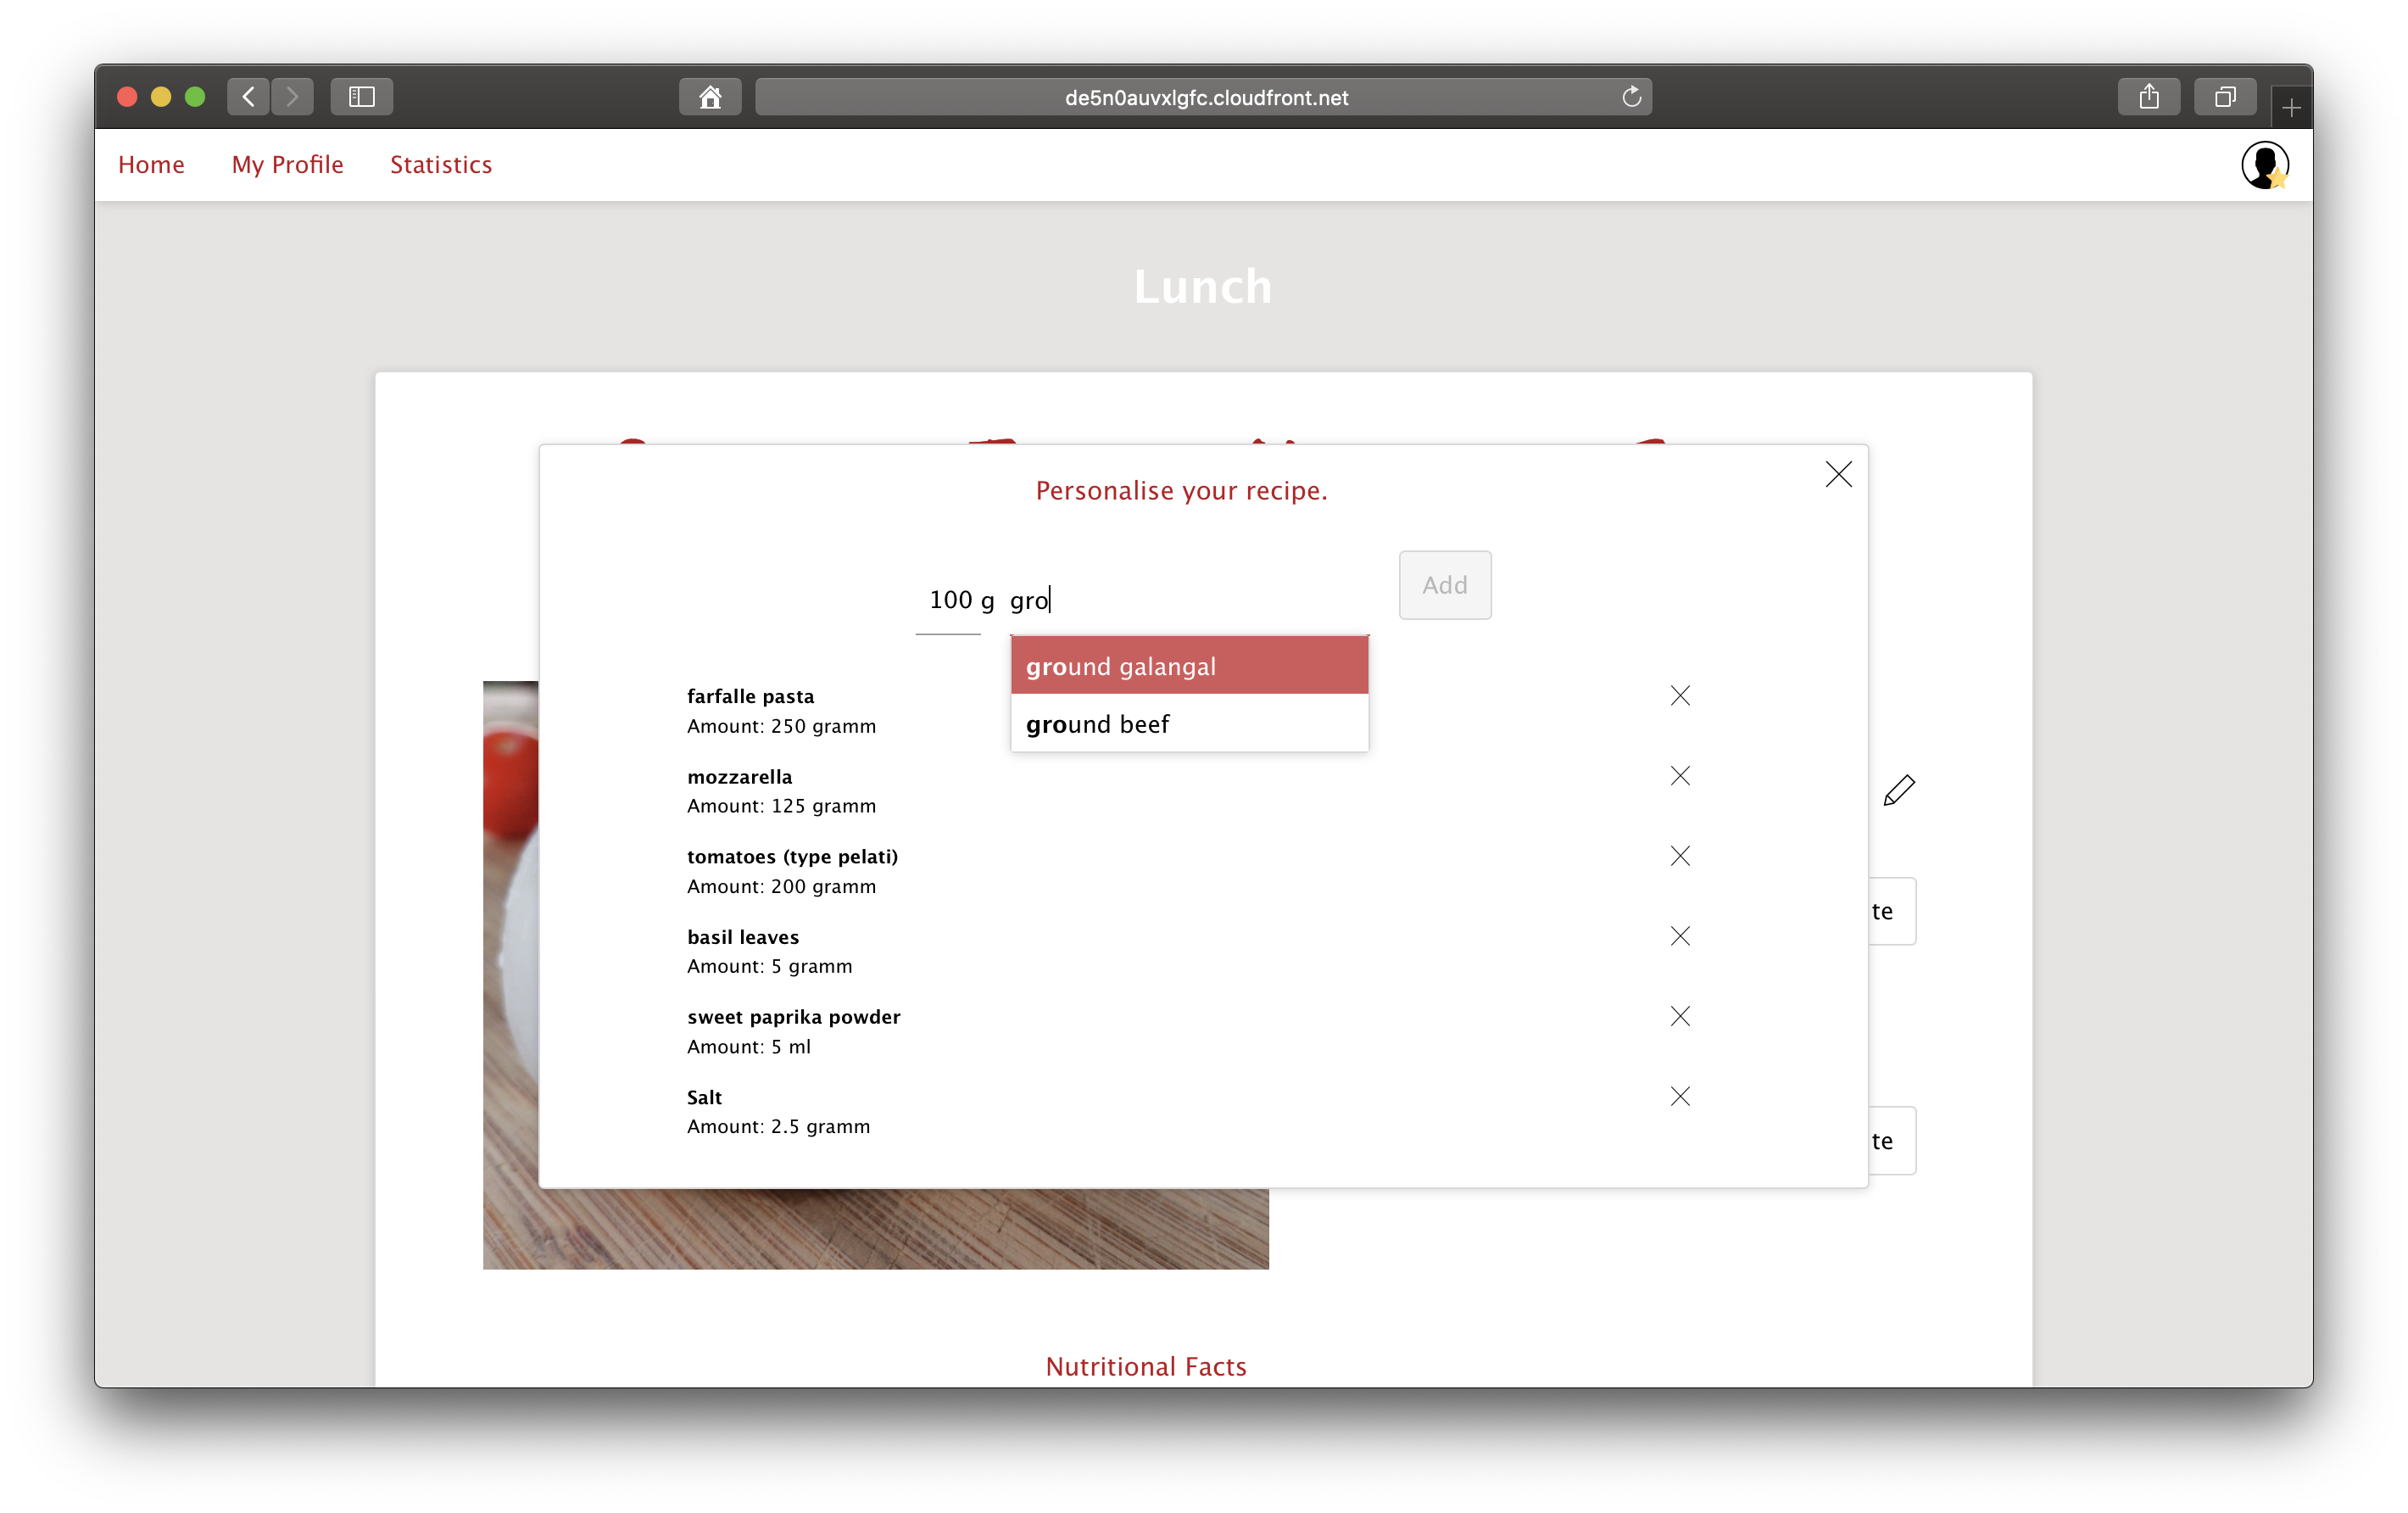
\includegraphics[scale=0.28]{Ressourcen/img/screenshots/screenshotK.png}
		\vspace{-3em}
		\caption{Recipe personalisation}
		\label{fig:personalisation}
	\end{center}
\end{figure}

Below the recipe details, the user can also find some nutritional facts consisting of graphs and statistics regarding the (modified) recipe. The user can click through three different representations of the nutritional composition of the currently shown recipe:
\begin{itemize}
\item \textbf{Pie chart}: This is the initially shown diagram which merely displays the ratio of carbohydrates, fats and proteins without additional numbers (see figure \ref{fig:detailedStatistics} - first screenshot).
\item \textbf{Table}: Here, the user can find the most important components of the nutrition table (see figure \ref{fig:detailedStatistics} - second screenshot).
\item \textbf{Bar graph}: This graph shows the most important nutrition components in percentage of the optimal daily intake of an adult based on the (Quelle einbinden, EU Guidelines). It also shows how much percent the user improved or deteriorated its personalized recipe with the current substitutions (see figure \ref{fig:detailedStatistics} - third screenshot).
\end{itemize}

\begin{figure}[H]
	\captionsetup{justification=centering}
	\begin{center}
		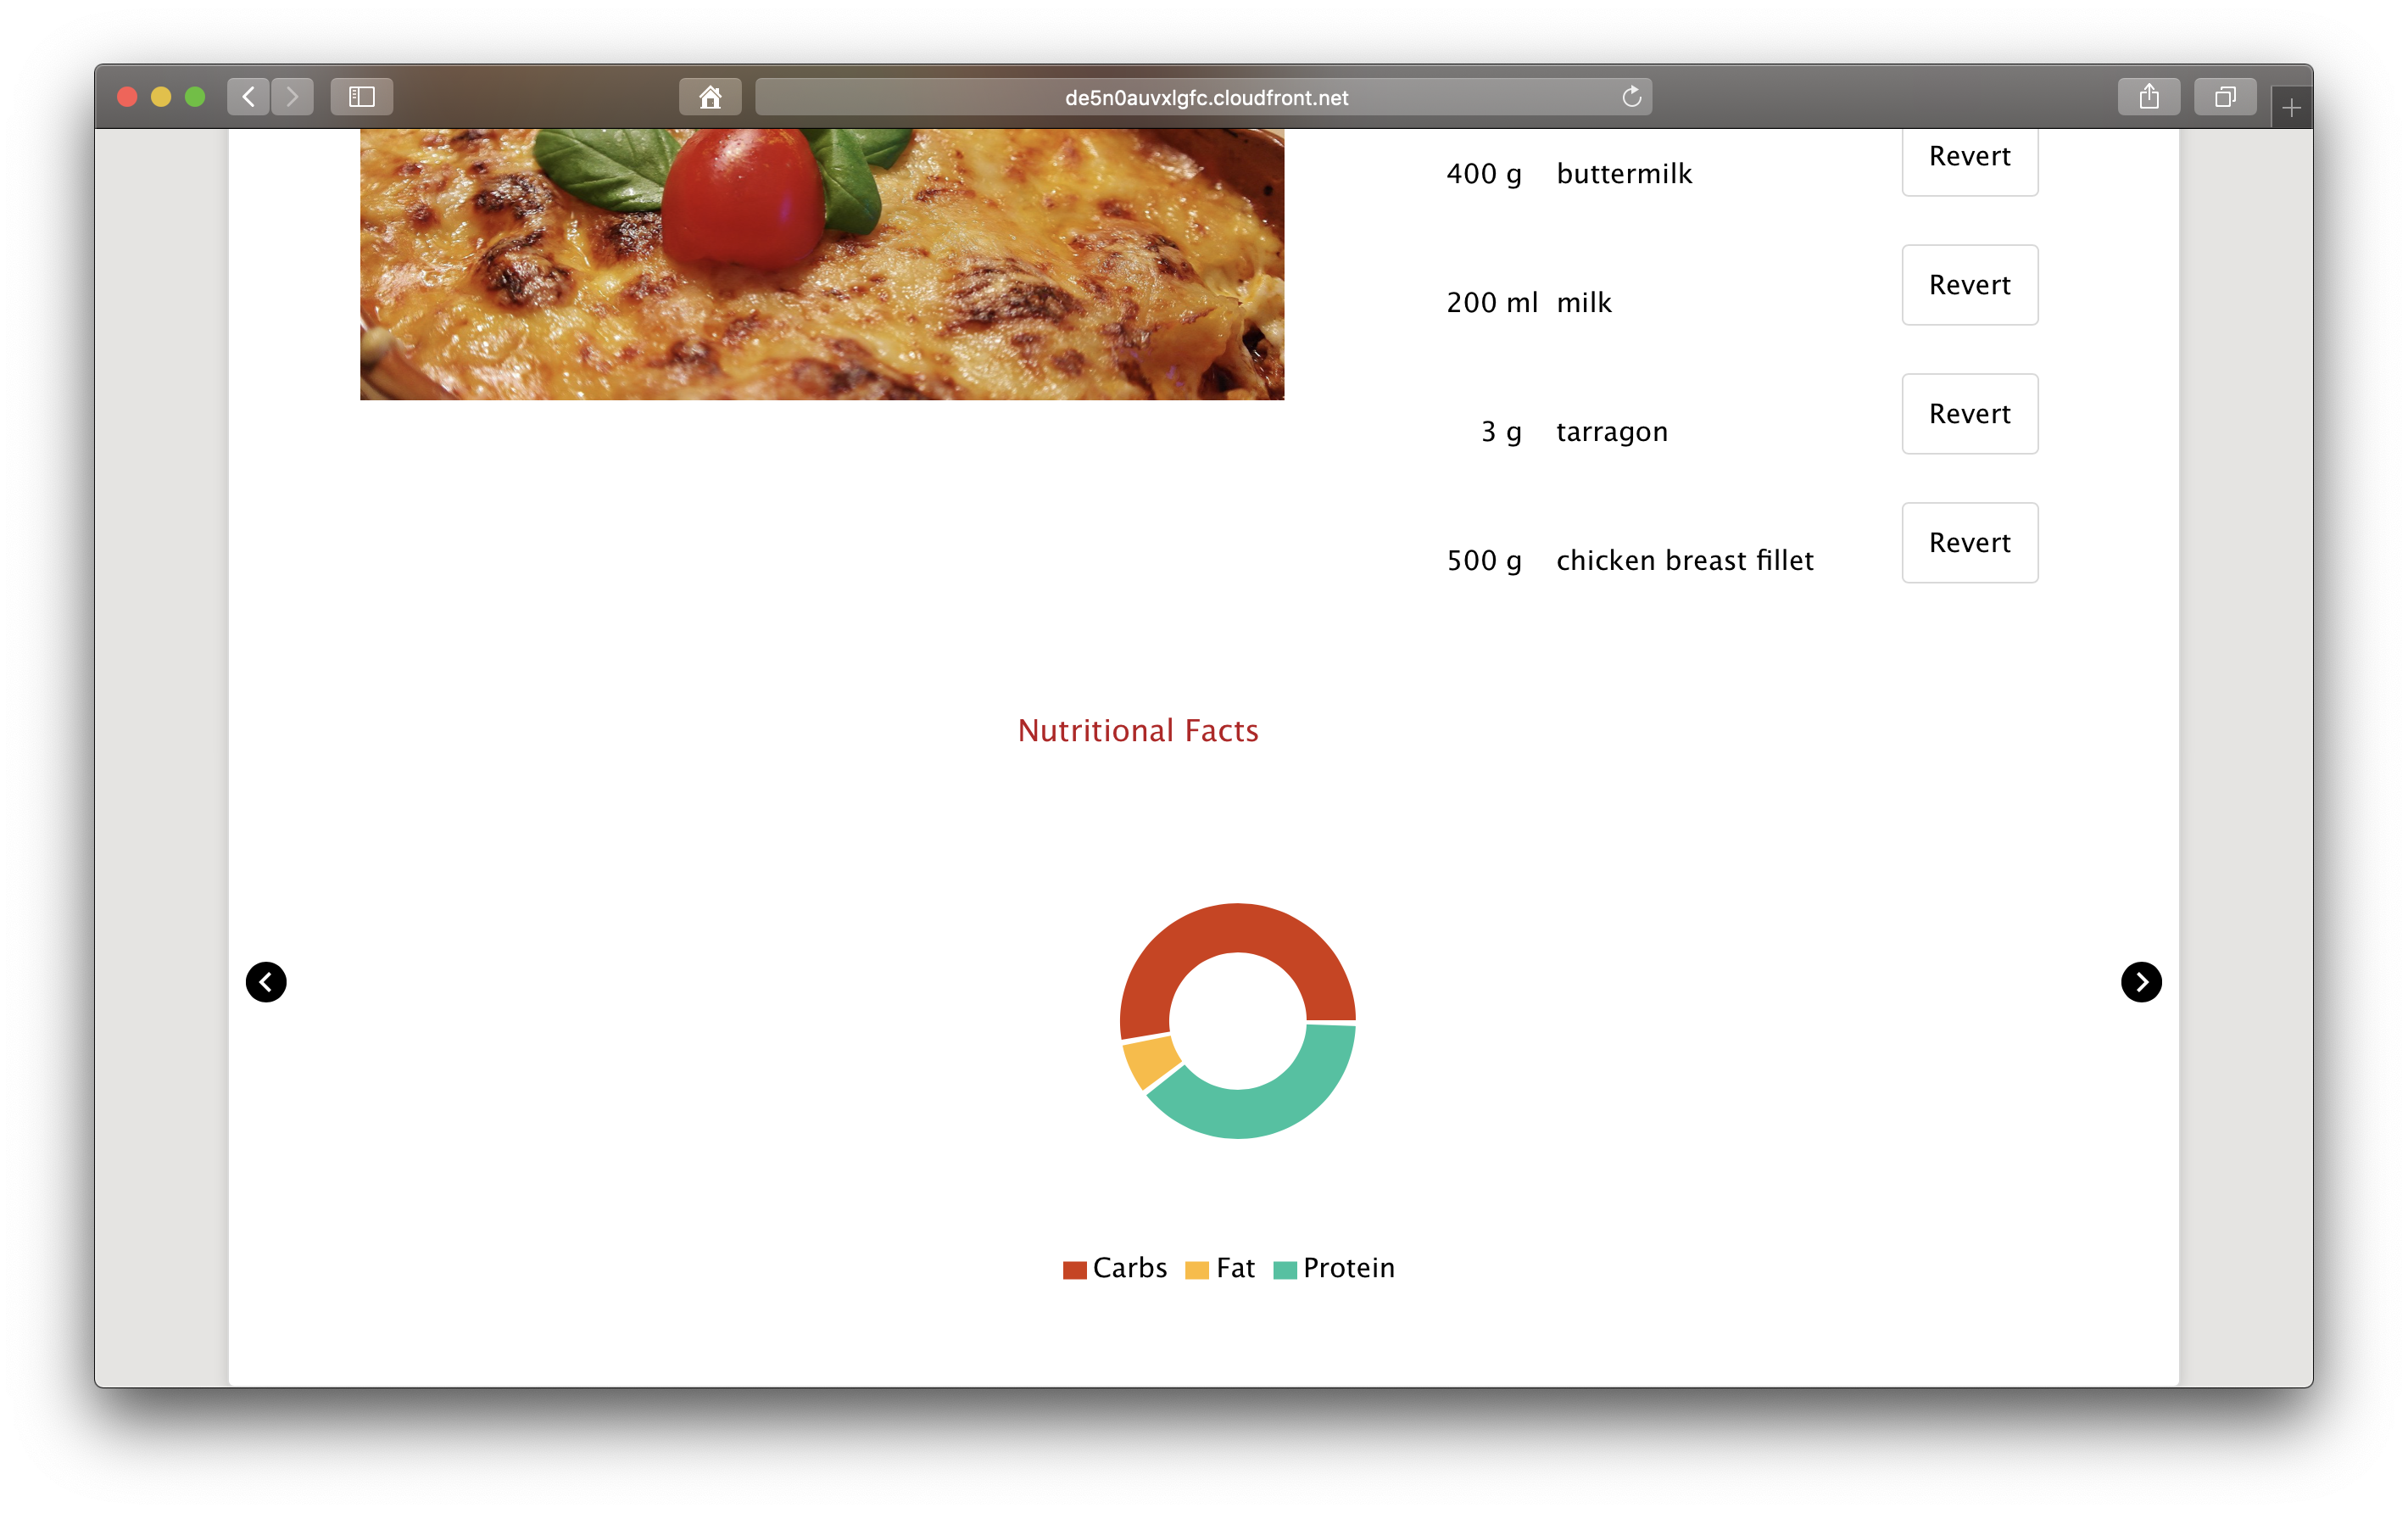
\includegraphics[scale=0.35]{Ressourcen/img/screenshots/screenshotL.png}\hfill
		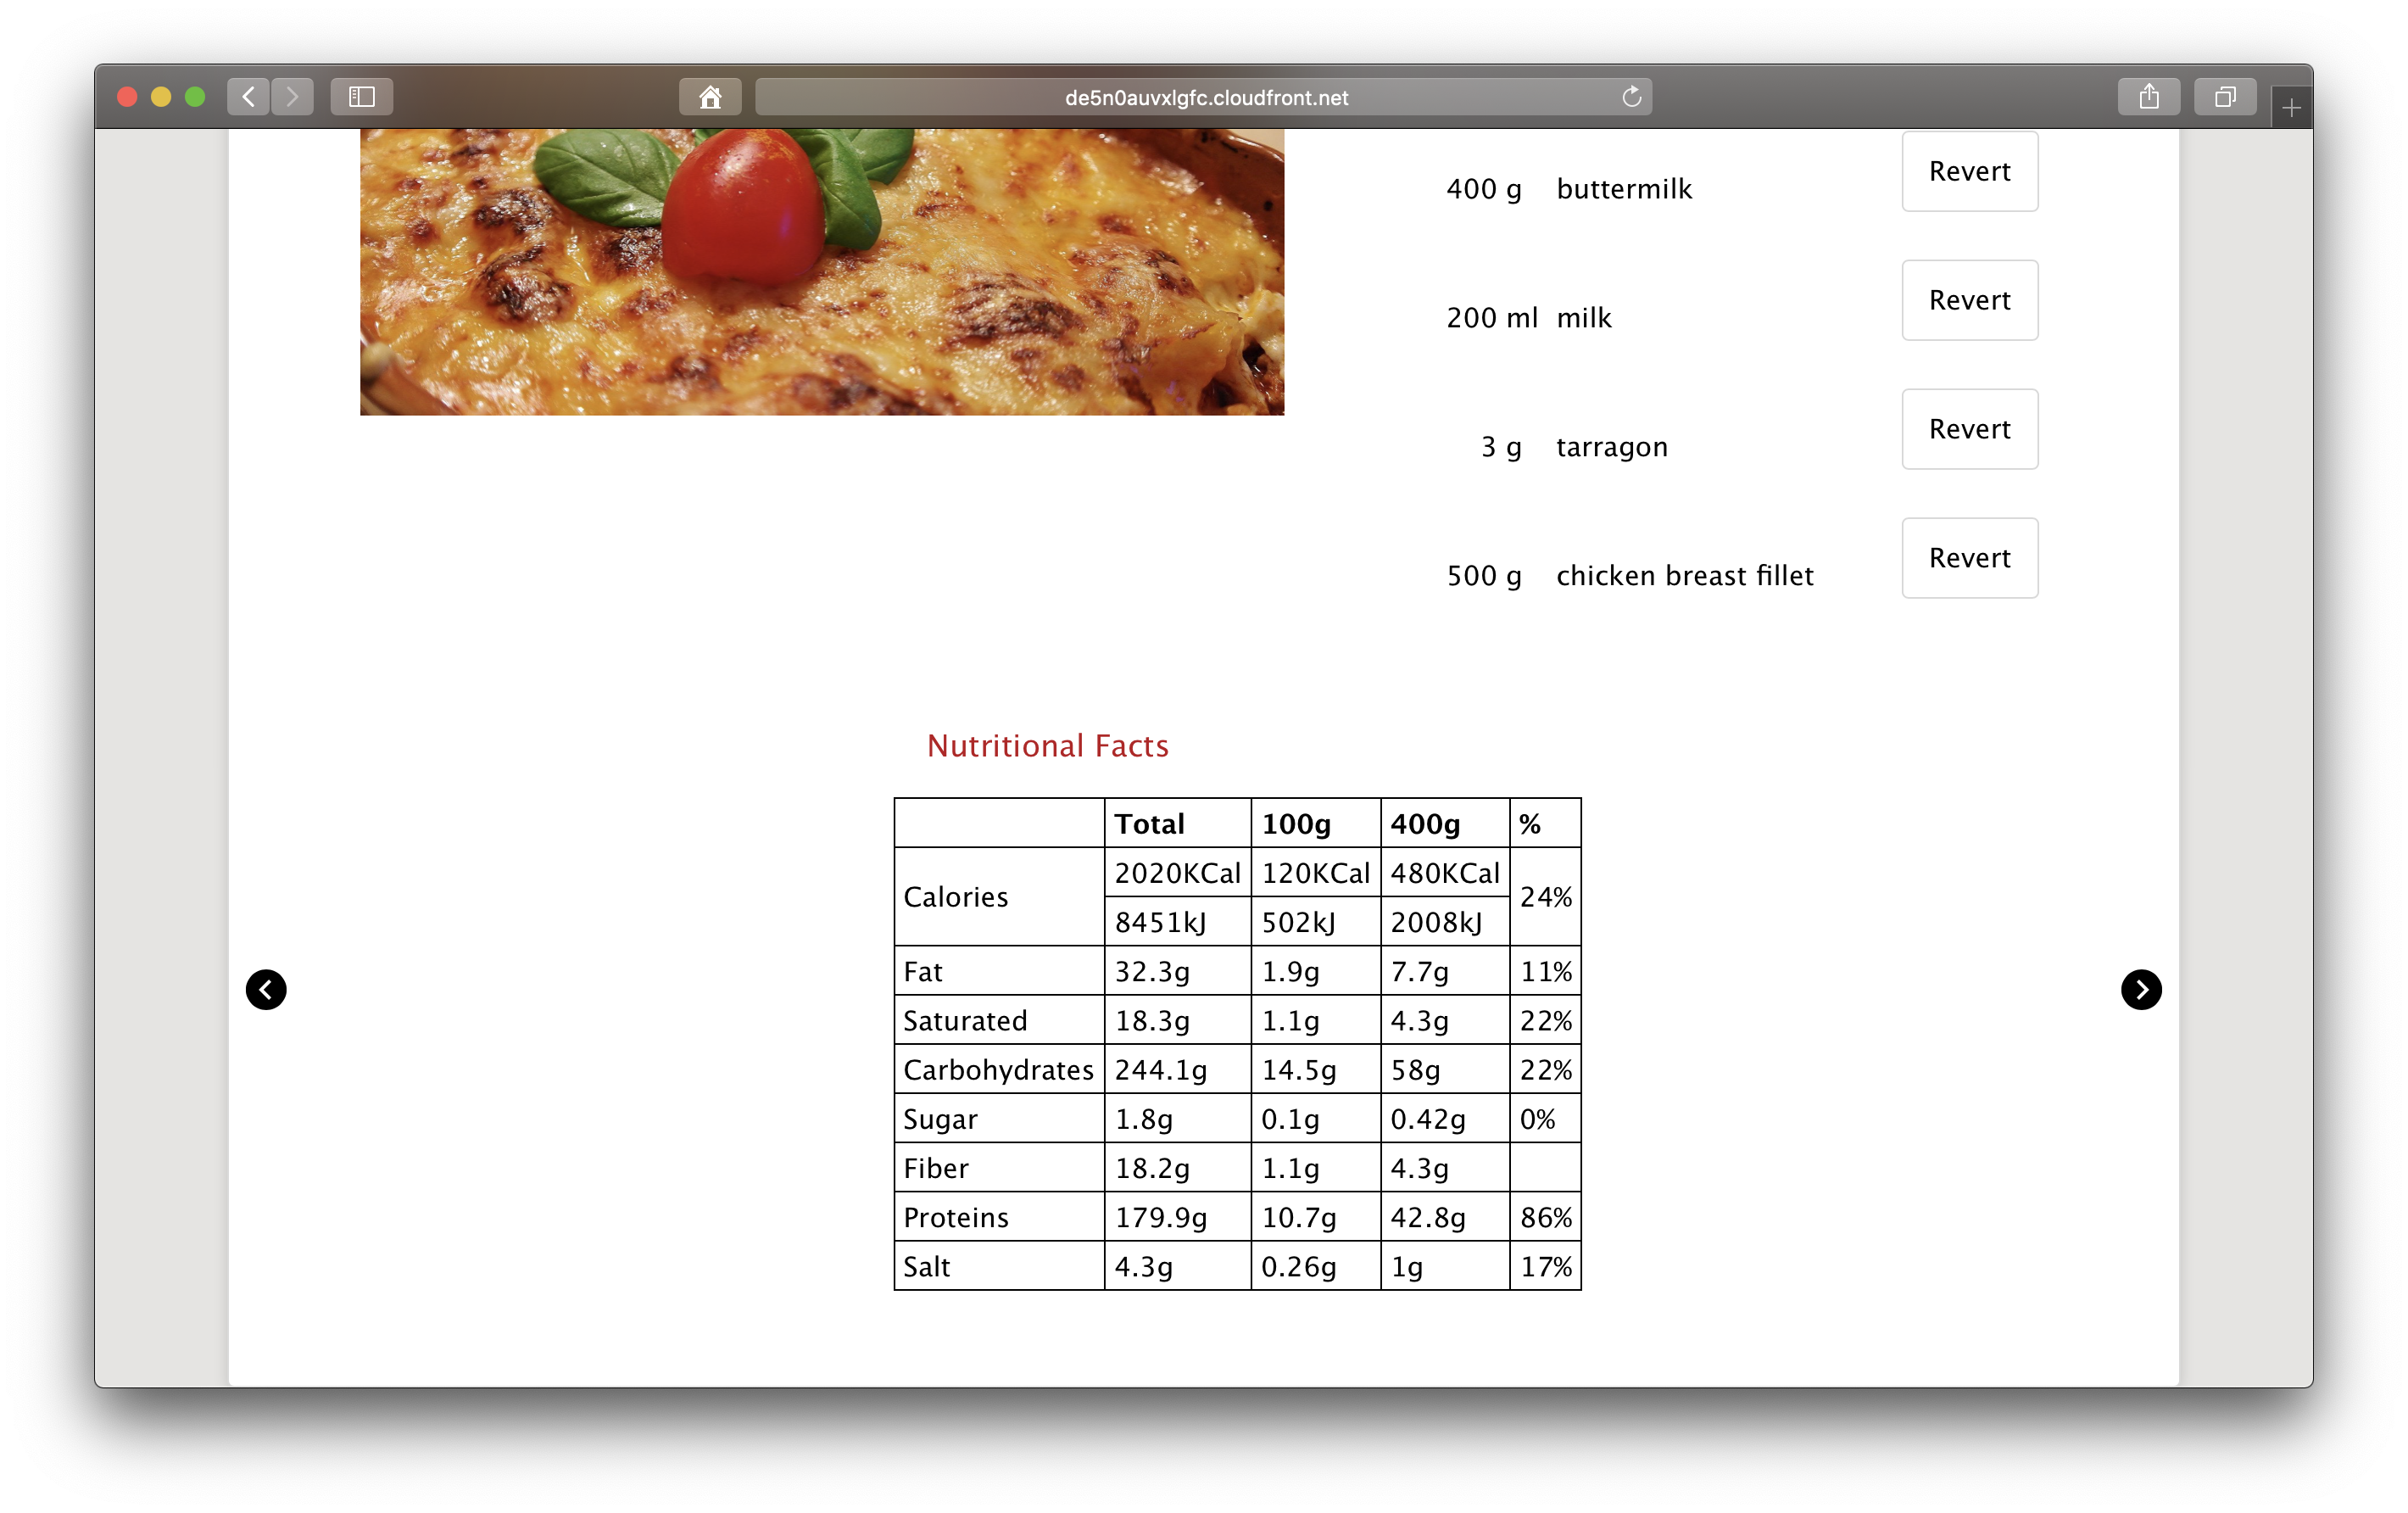
\includegraphics[scale=0.35]{Ressourcen/img/screenshots/screenshotM.png}\hfill
		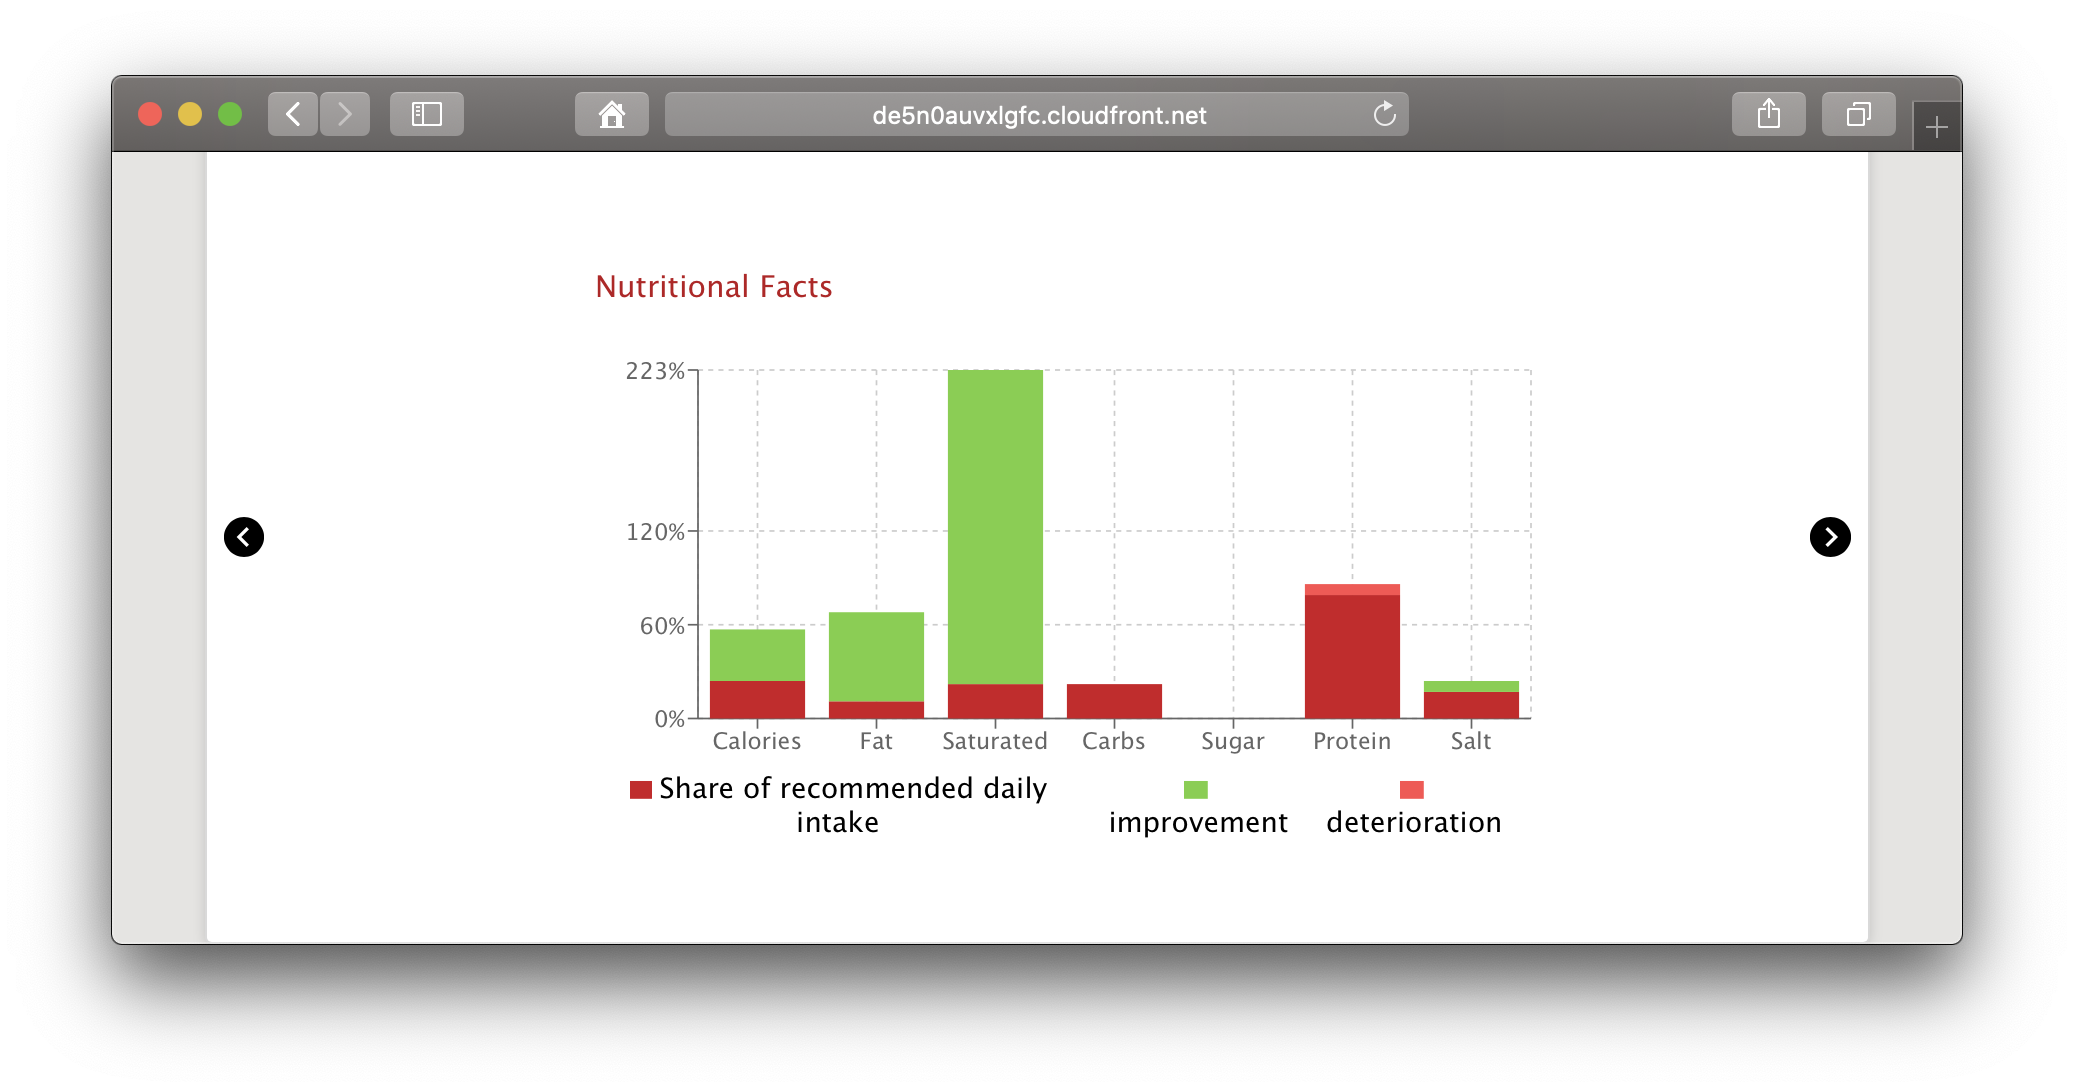
\includegraphics[scale=0.35]{Ressourcen/img/screenshots/screenshotN.png}
		\vspace{-3em}
	\end{center}
	\caption{Pie chart, table and bar graph for a recipe}
	\label{fig:detailedStatistics}
\end{figure}

\subsection*{Profile page}
\vspace{0.5em}
\begin{figure}[H]
	\captionsetup{justification=centering}
	\begin{center}
		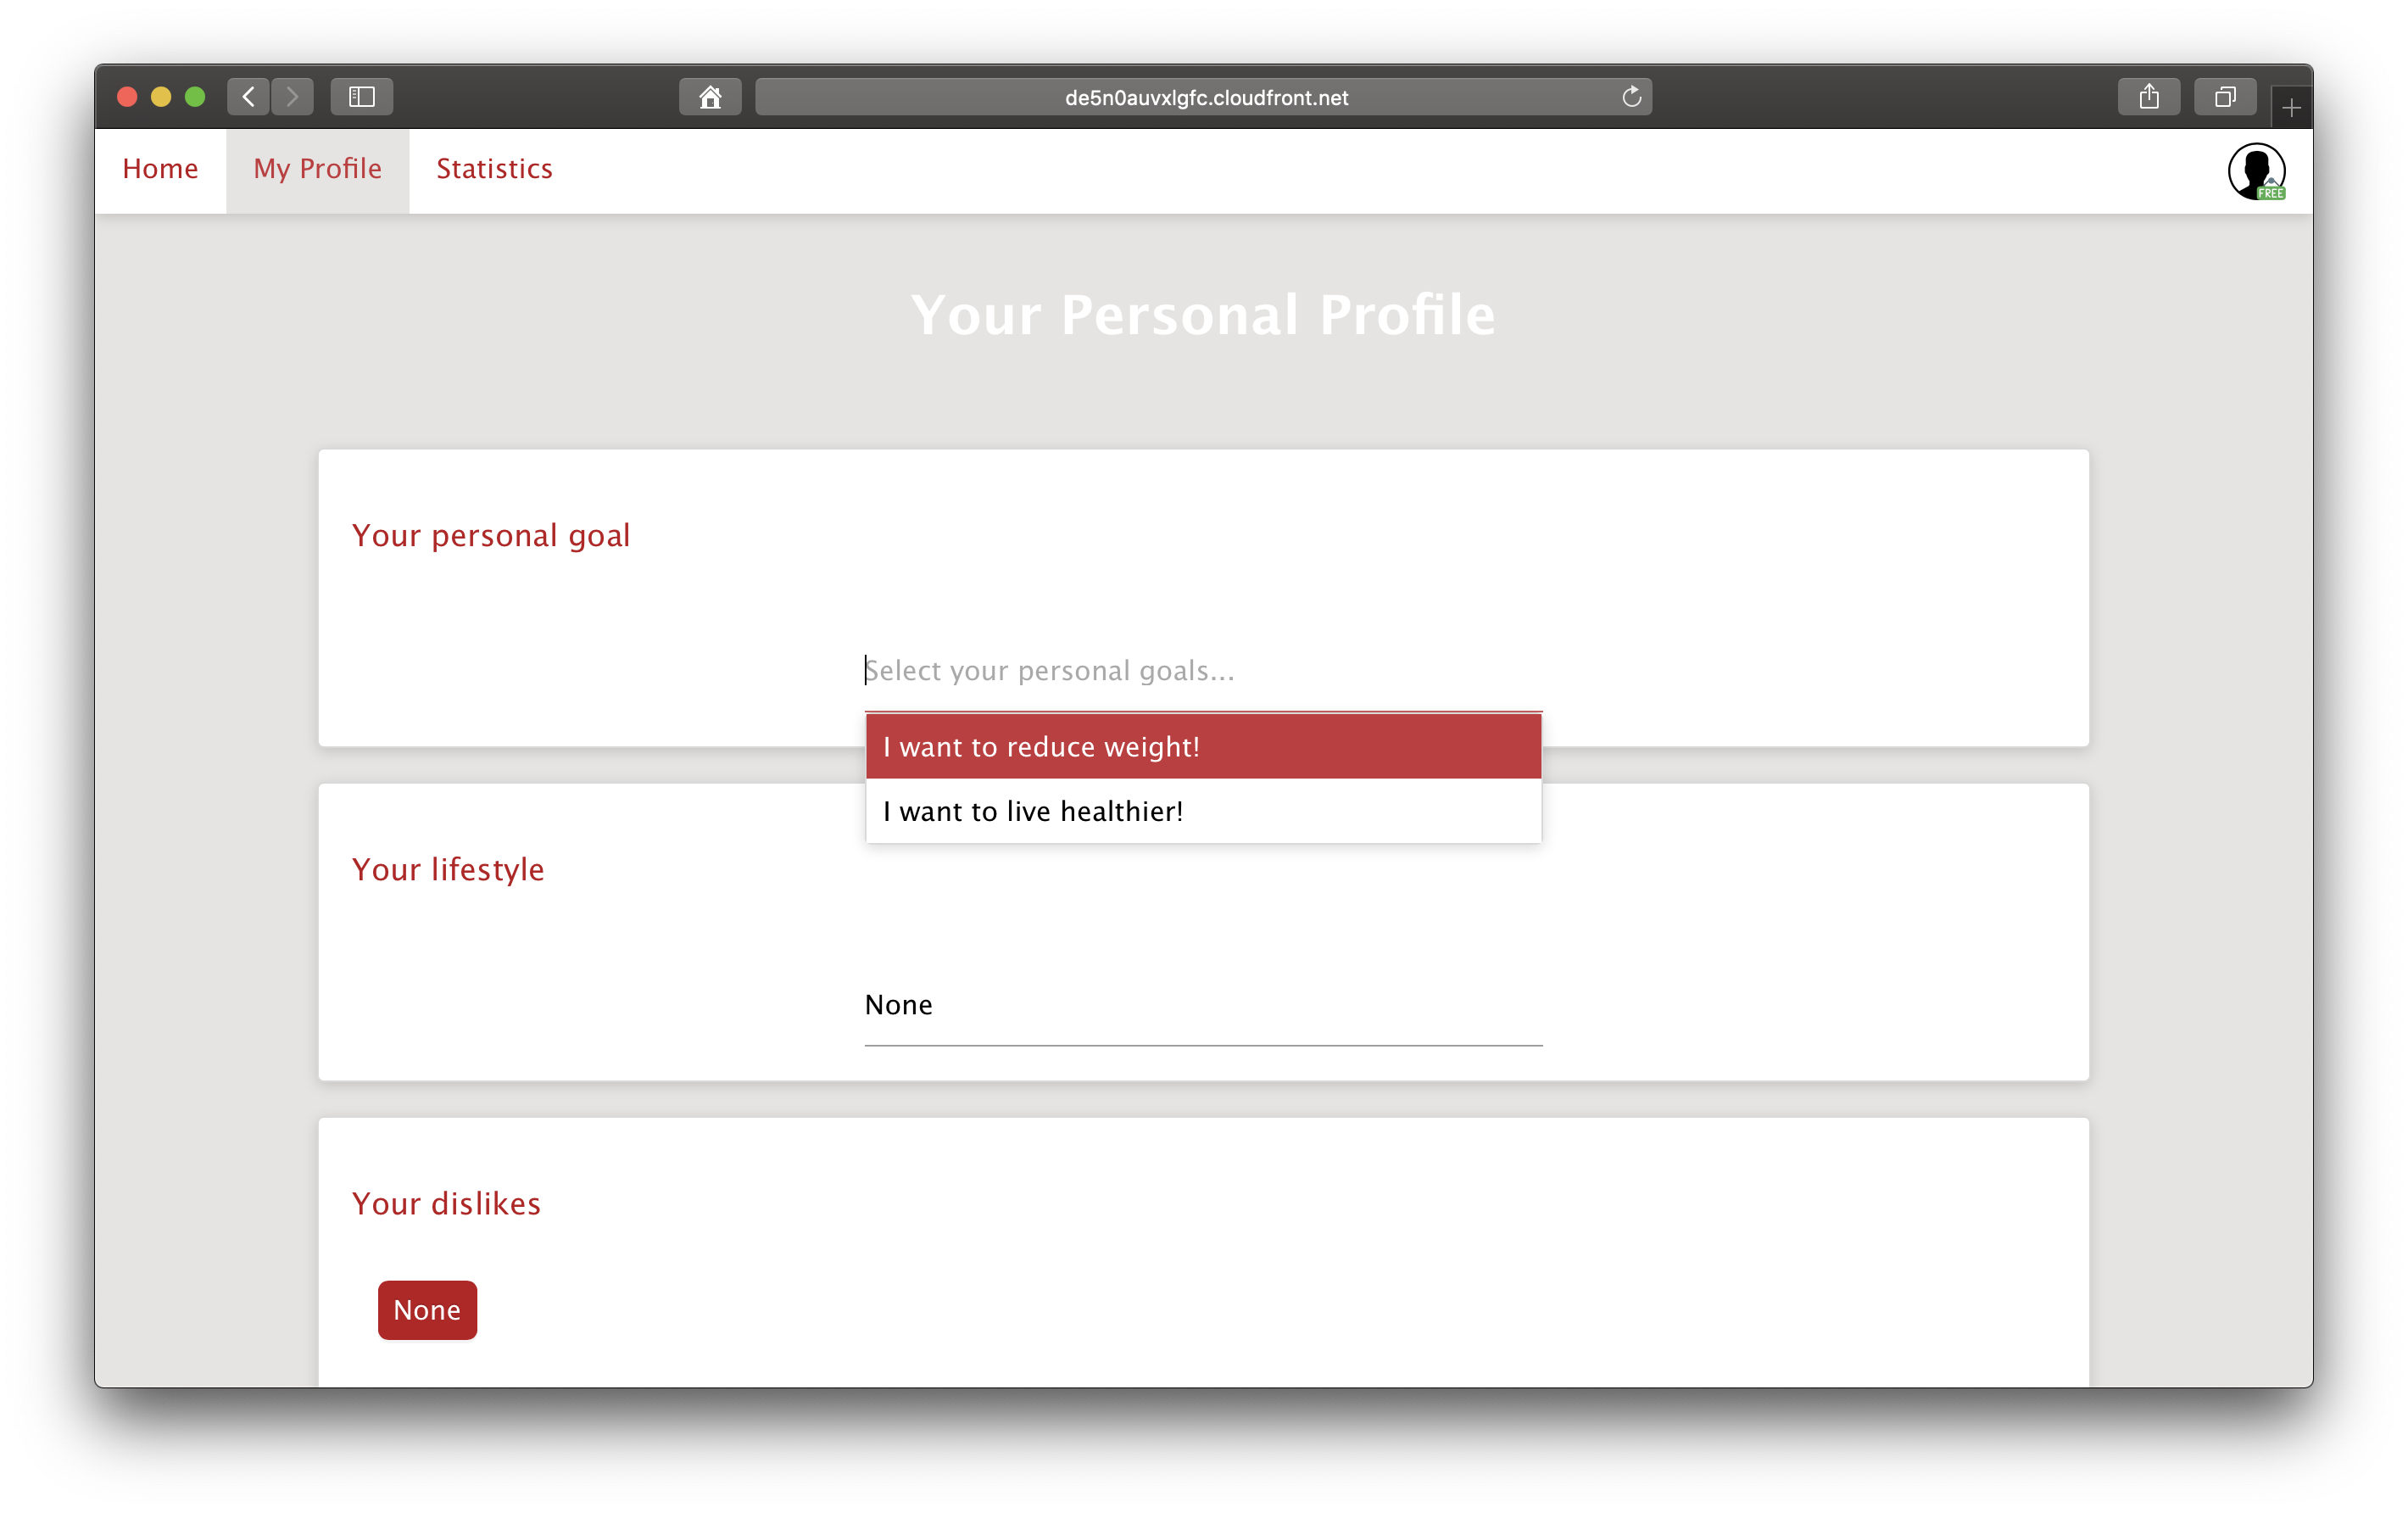
\includegraphics[scale=0.30]{Ressourcen/img/screenshots/screenshotO.png}
		\vspace{-2em}
		\caption{Profile page goal and lifestyle}
	\end{center}
\end{figure}
\vspace{-2em}
As already mentioned above, the user first has to select a personal goal before the substitution process becomes available. To improve the received substitutes from the substitution algorithm, it is advised for the user to also insert additional personal information, currently consisting of:

\begin{itemize}
\item \textbf{Goal}: Reduce weight or live healthier.
\item \textbf{Lifestyle}: Vegetarian, low carb or vegan
\item \textbf{Dislikes}: A list of ingredients he does not like and therefore wishes to not be shown as substitutes.
\item \textbf{Allergies}: A list of ingredients he can not eat and therefore should not be shown as substitutes.
\end{itemize}

Changes to a user’s profile will be saved automatically and can always be changed again.

\begin{figure}[H]
	\captionsetup{justification=centering}
	\begin{center}
		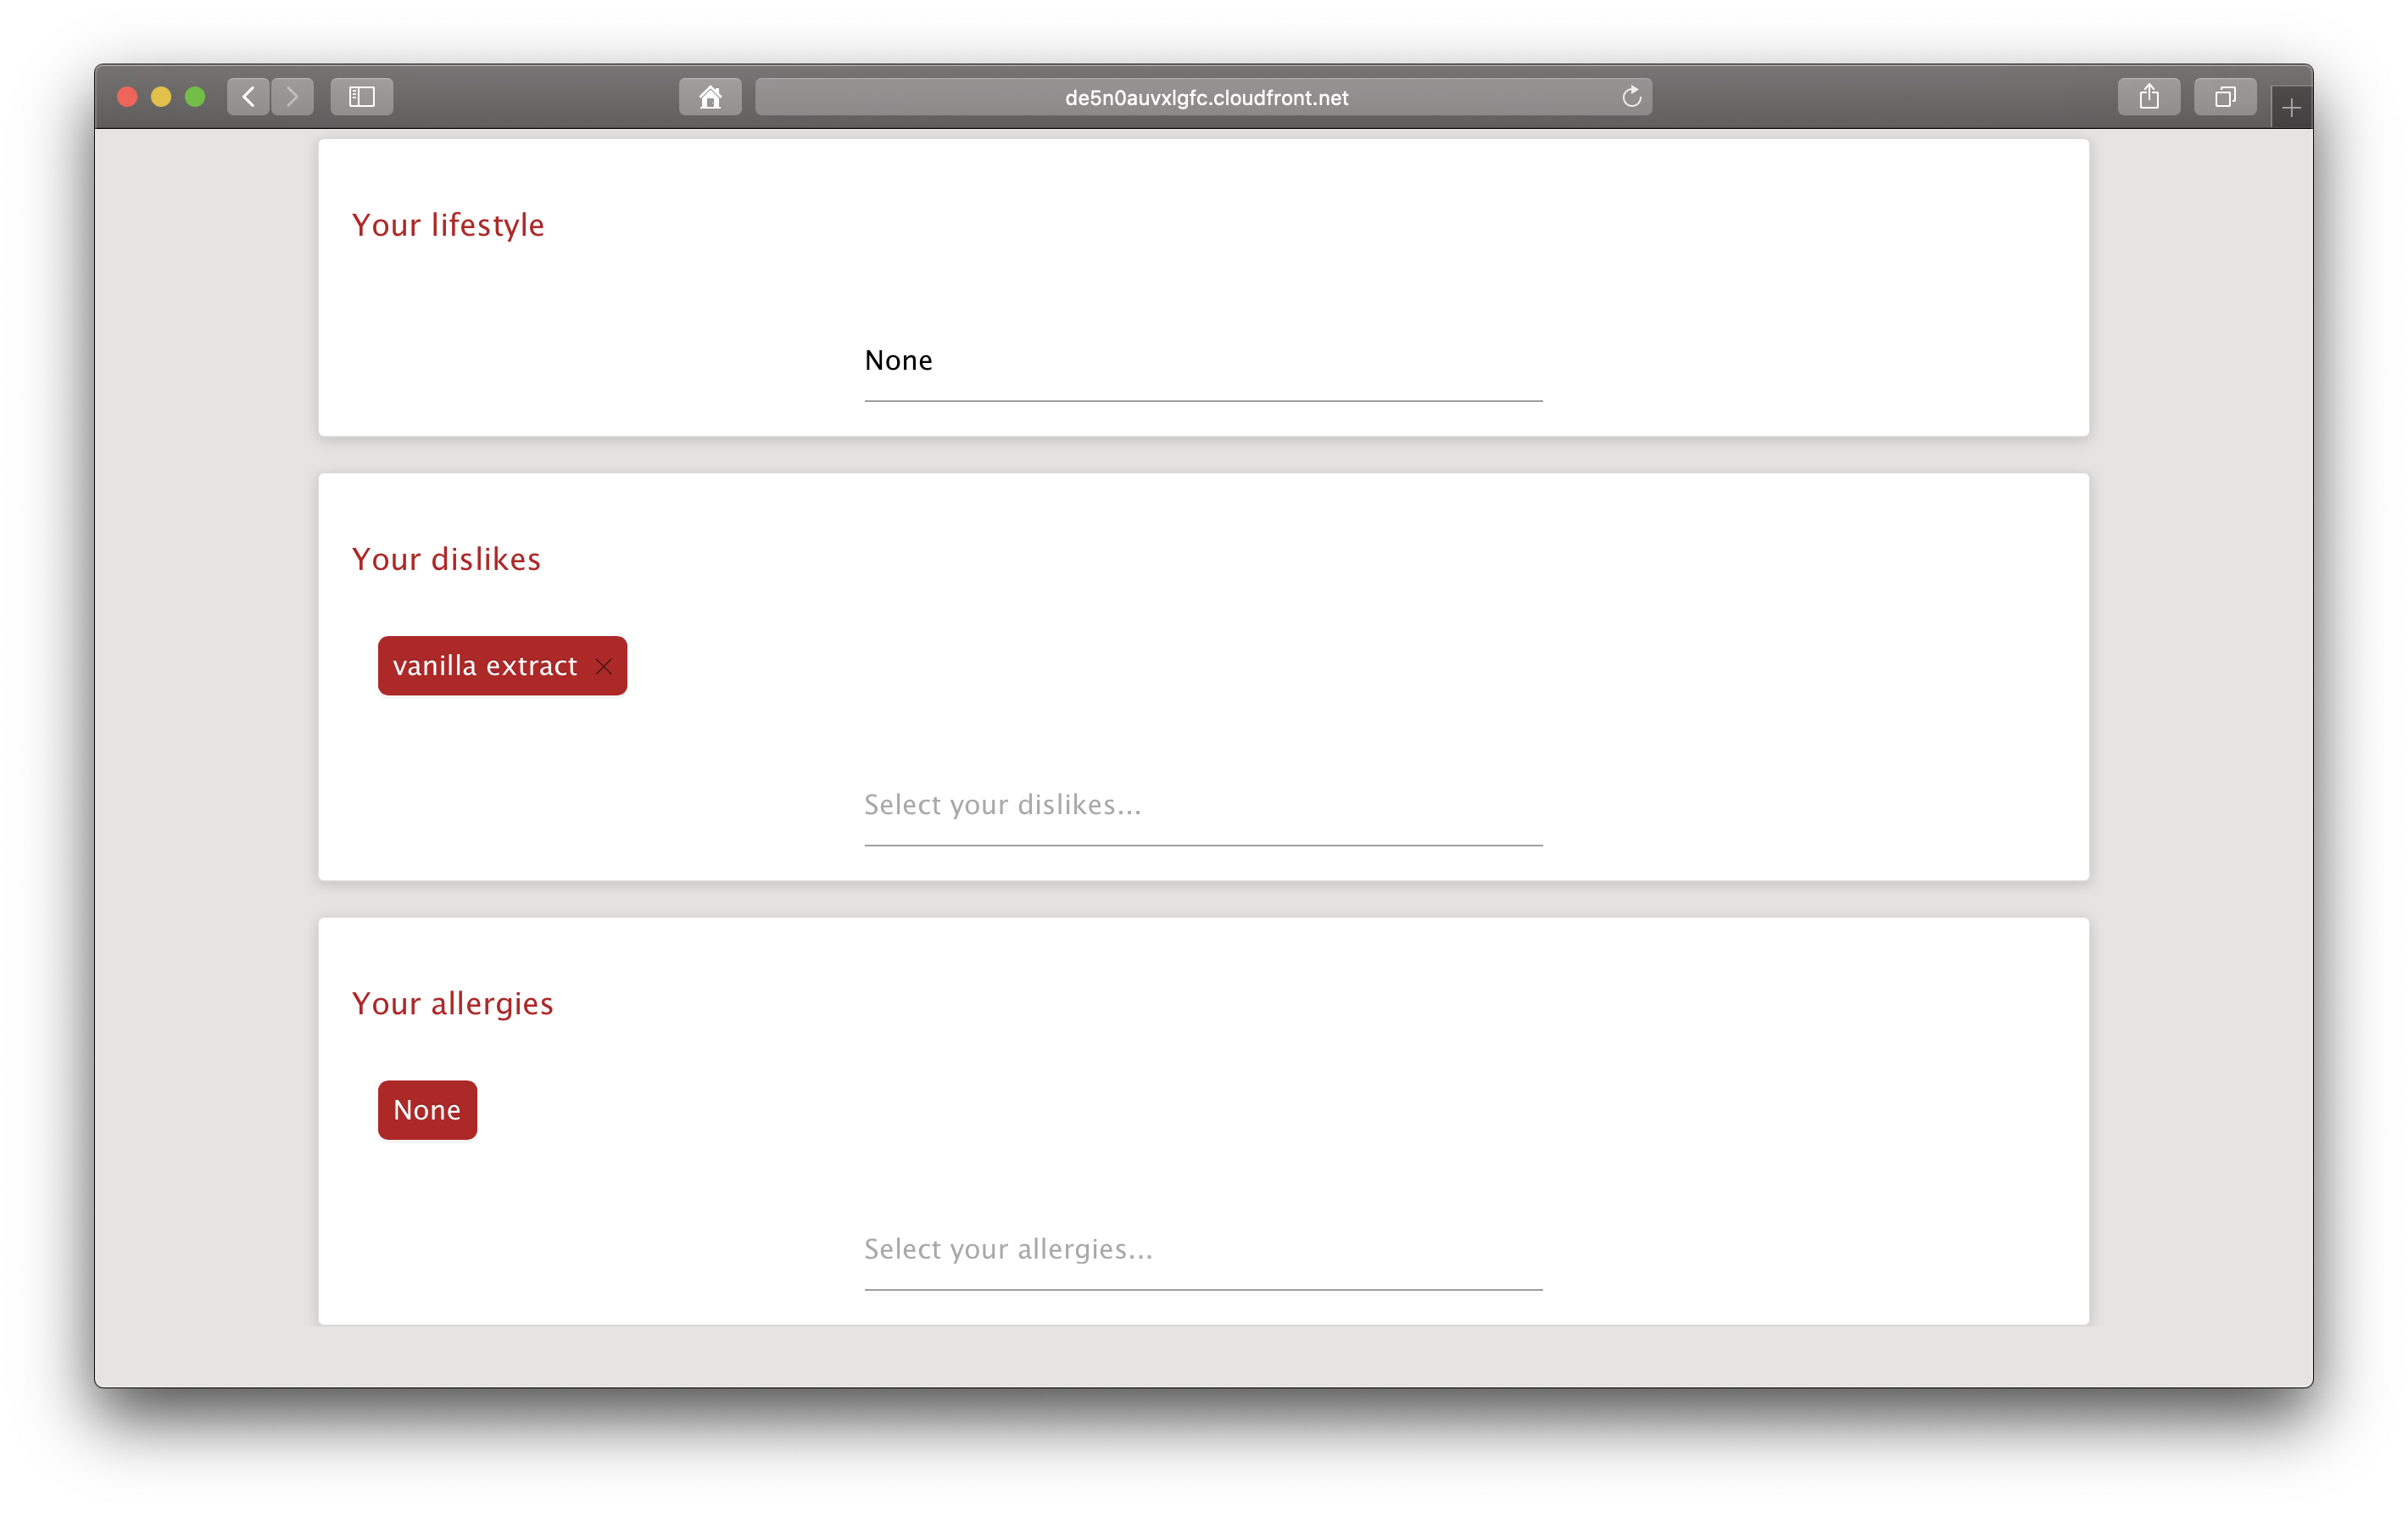
\includegraphics[scale=0.30]{Ressourcen/img/screenshots/screenshotP.png}
		\vspace{-2em}
		\caption{Profile page dislikes and allergies}
	\end{center}
\end{figure}

\subsection*{Statistics page}
\vspace{0.5em}
\begin{figure}[H]
	\captionsetup{justification=centering}
	\begin{center}
		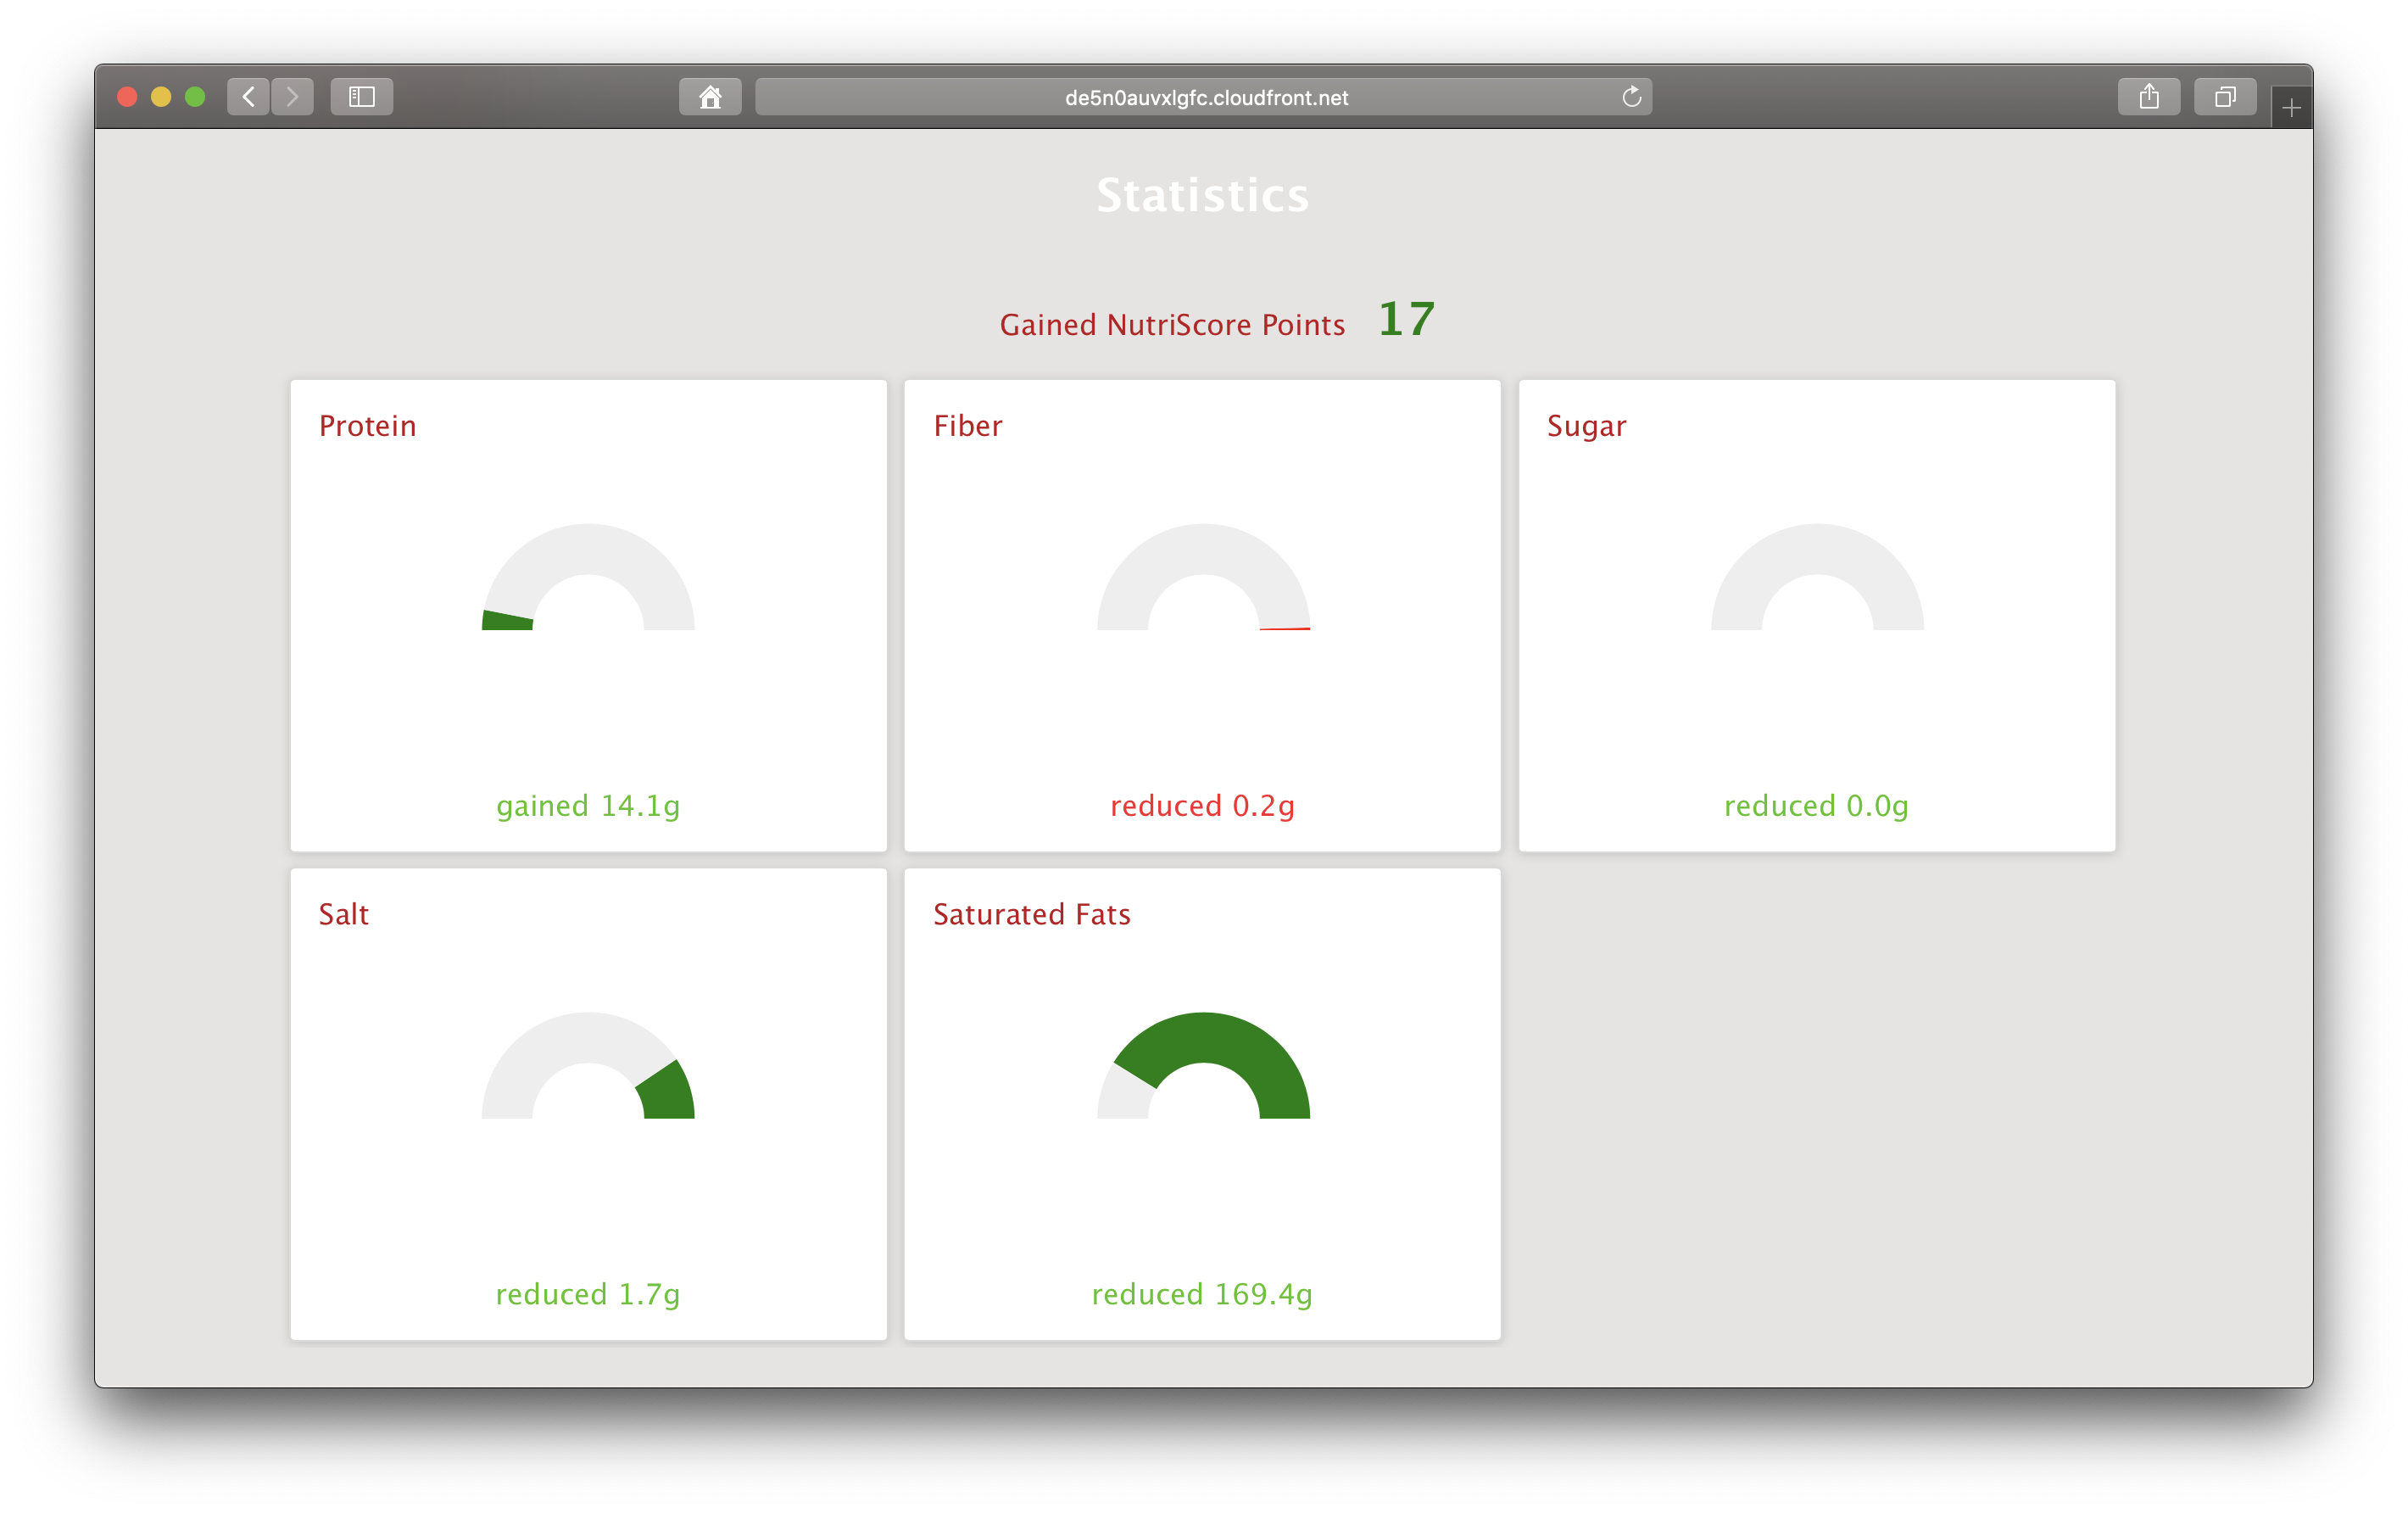
\includegraphics[scale=0.30]{Ressourcen/img/screenshots/screenshotQ.png}
		\vspace{-3em}
		\caption{User statistics}
	\end{center}
\end{figure}
		\vspace{-2em}
By clicking on \texttt{Statistics} in the navbar, a user can get an overview about its nutritional career with Foodo. Throughout the substitution history, some personal nutritional data will be gathered and stored for each user. Through the statistics, one can see how many NutriScore points the user has improved over all recipes in total as well as the amount of the five main nutritional values. Improvements, such as gaining protein or fiber and reducing sugar, salt or saturated fats, will be highlighted in green while negative changes will be highlighted in red.

\subsection*{PayPal Premium}
\vspace{0.5em}
\begin{figure}[H]
	\captionsetup{justification=centering}
	\begin{center}
		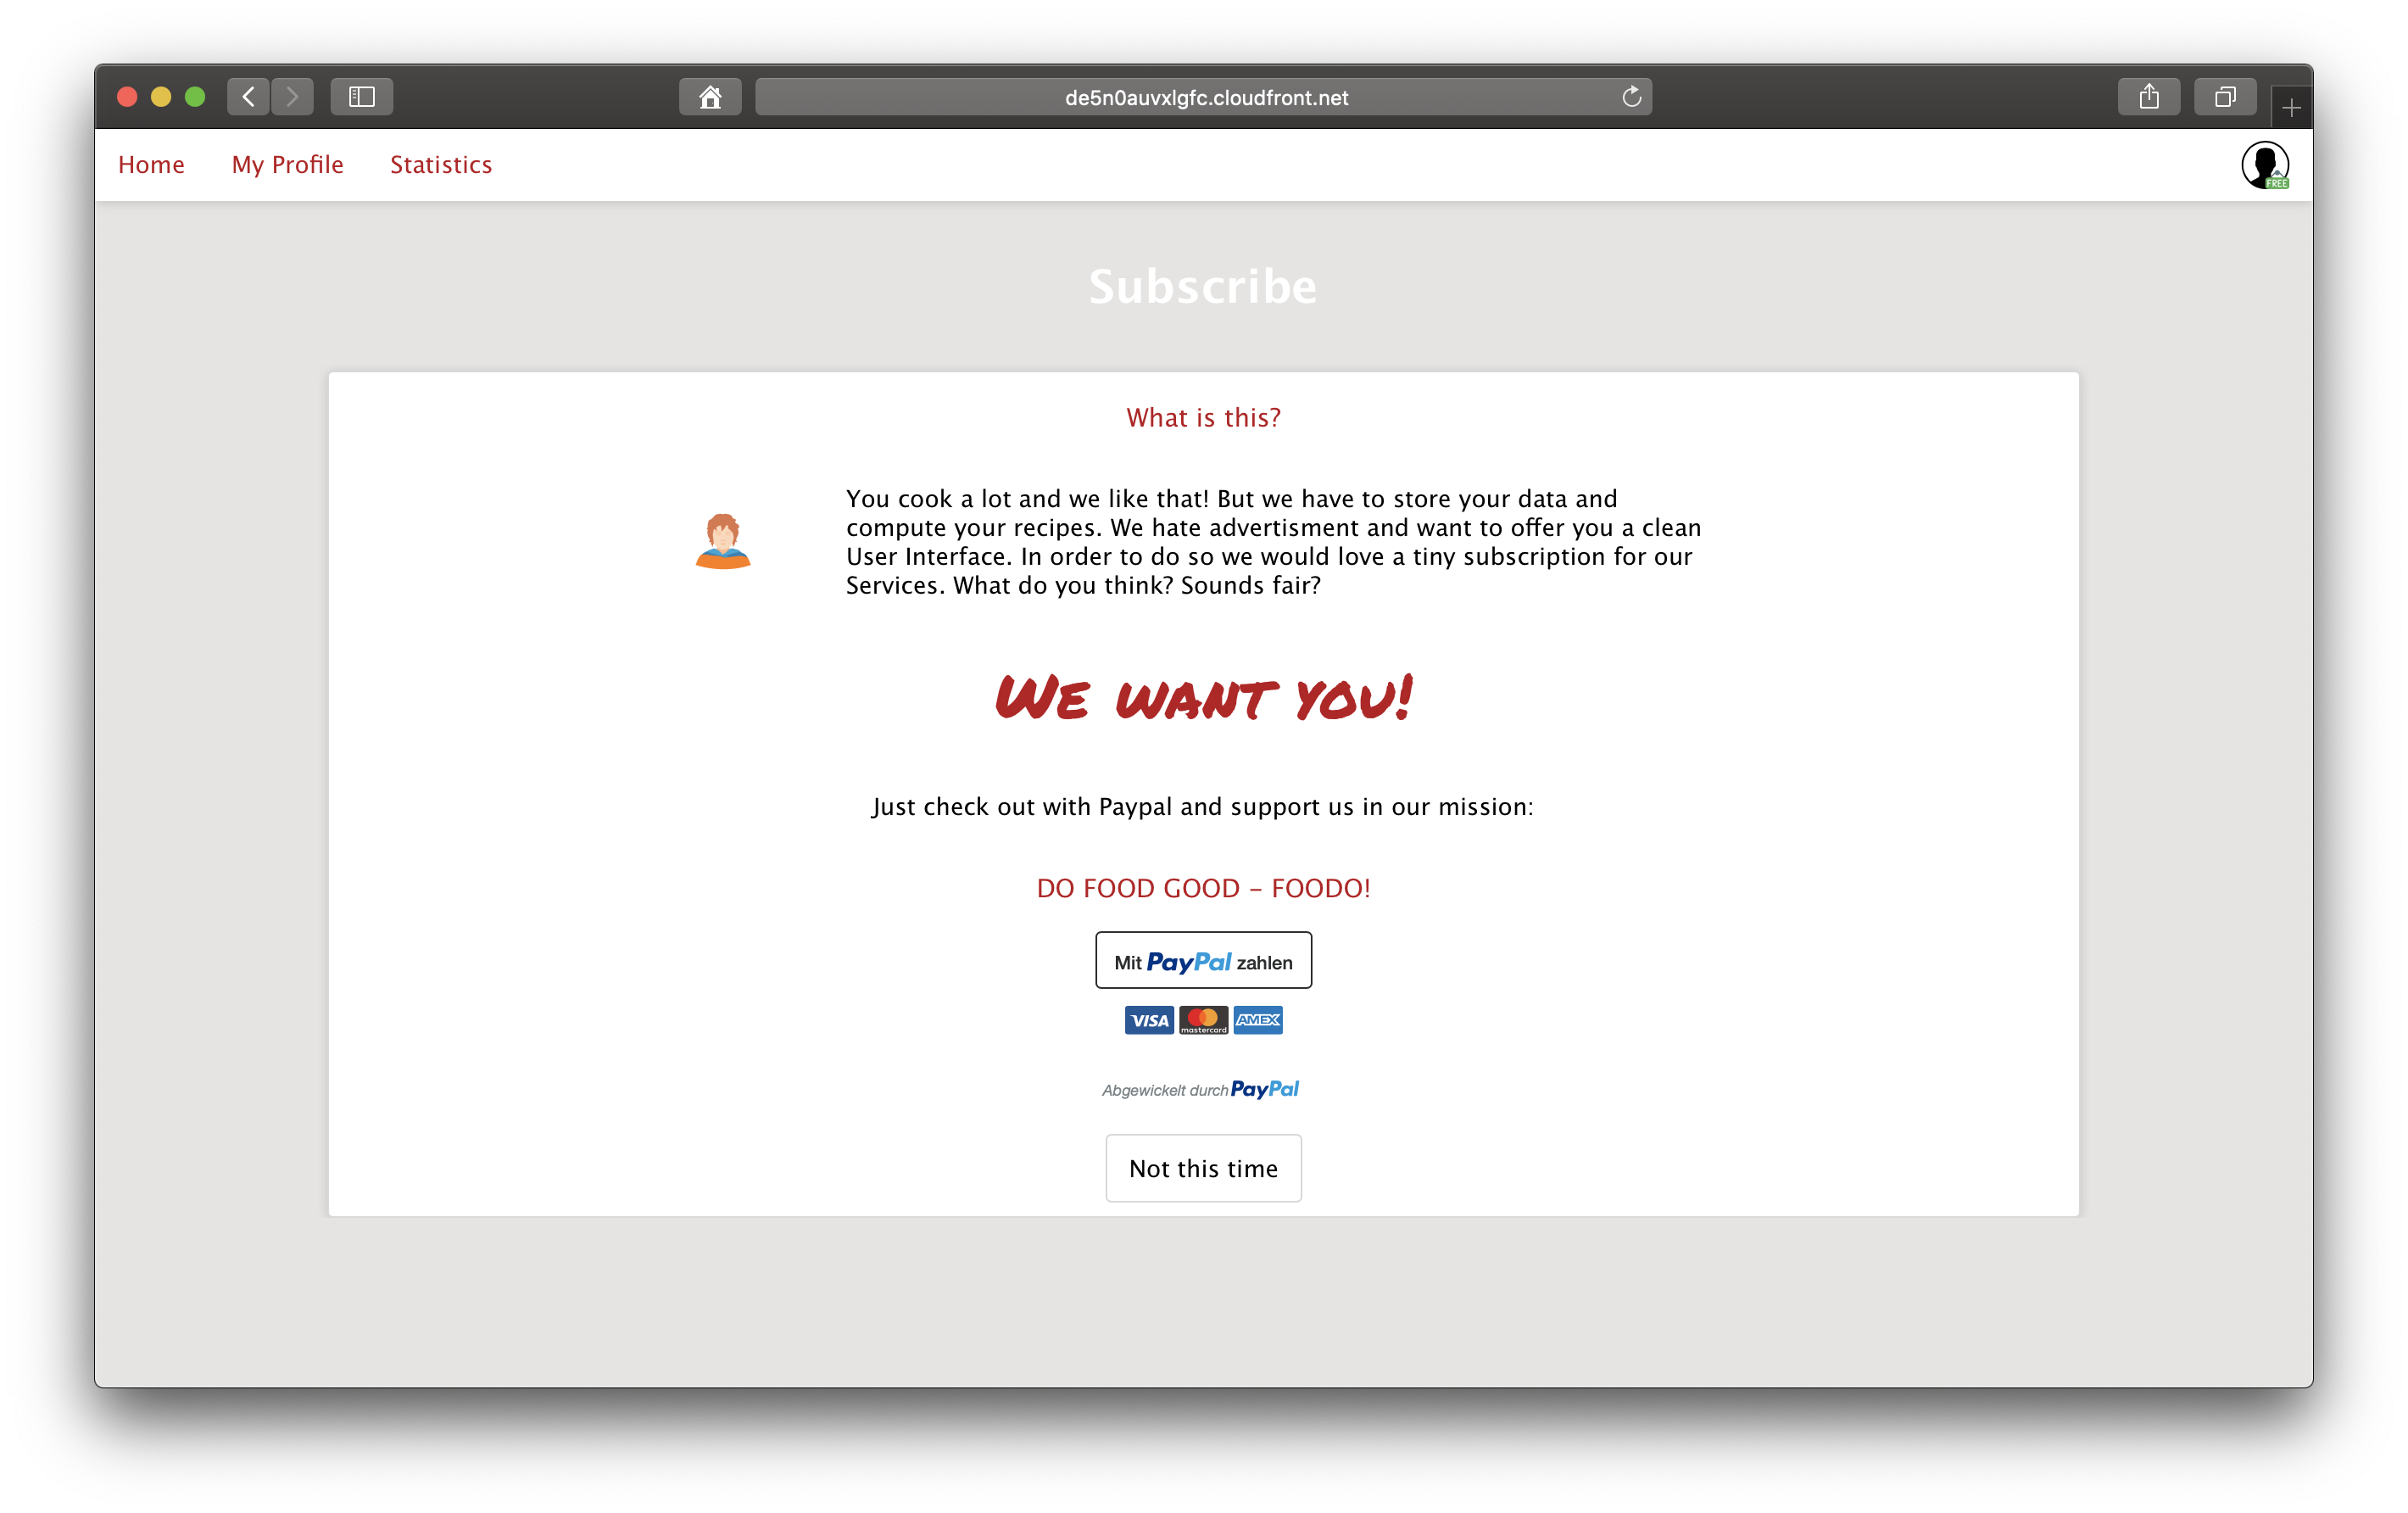
\includegraphics[scale=0.25]{Ressourcen/img/screenshots/screenshotR.png}
		\vspace{-2em}
		\caption{Premium opportunity}
		\label{fig:paypal}
	\end{center}
\end{figure}
After a specified free-to-use period, the user will see the popup shown in figure \ref{fig:paypal} where he can acquire a premium status through subscribing to the Foodo Paypal subscription plan. This will change the \texttt{Free} label next to the profile icon in the upper right corner to a star and will help the developer team to implement additional features. Currently, the free-to-use period allows the user to have up to five personalized recipes and the popup will show when the user tries to view more recipes. It is also to mention that the popup is currently skippable and the subscription plan is not mandatory but voluntary.  
\clearpage
\subsection*{Mobile version}
Foodo is also available for all mobile devices with access to a web browser. Some examples are shown in the figures below.

\begin{figure}[htp]
	\captionsetup{justification=centering}
	\centering
		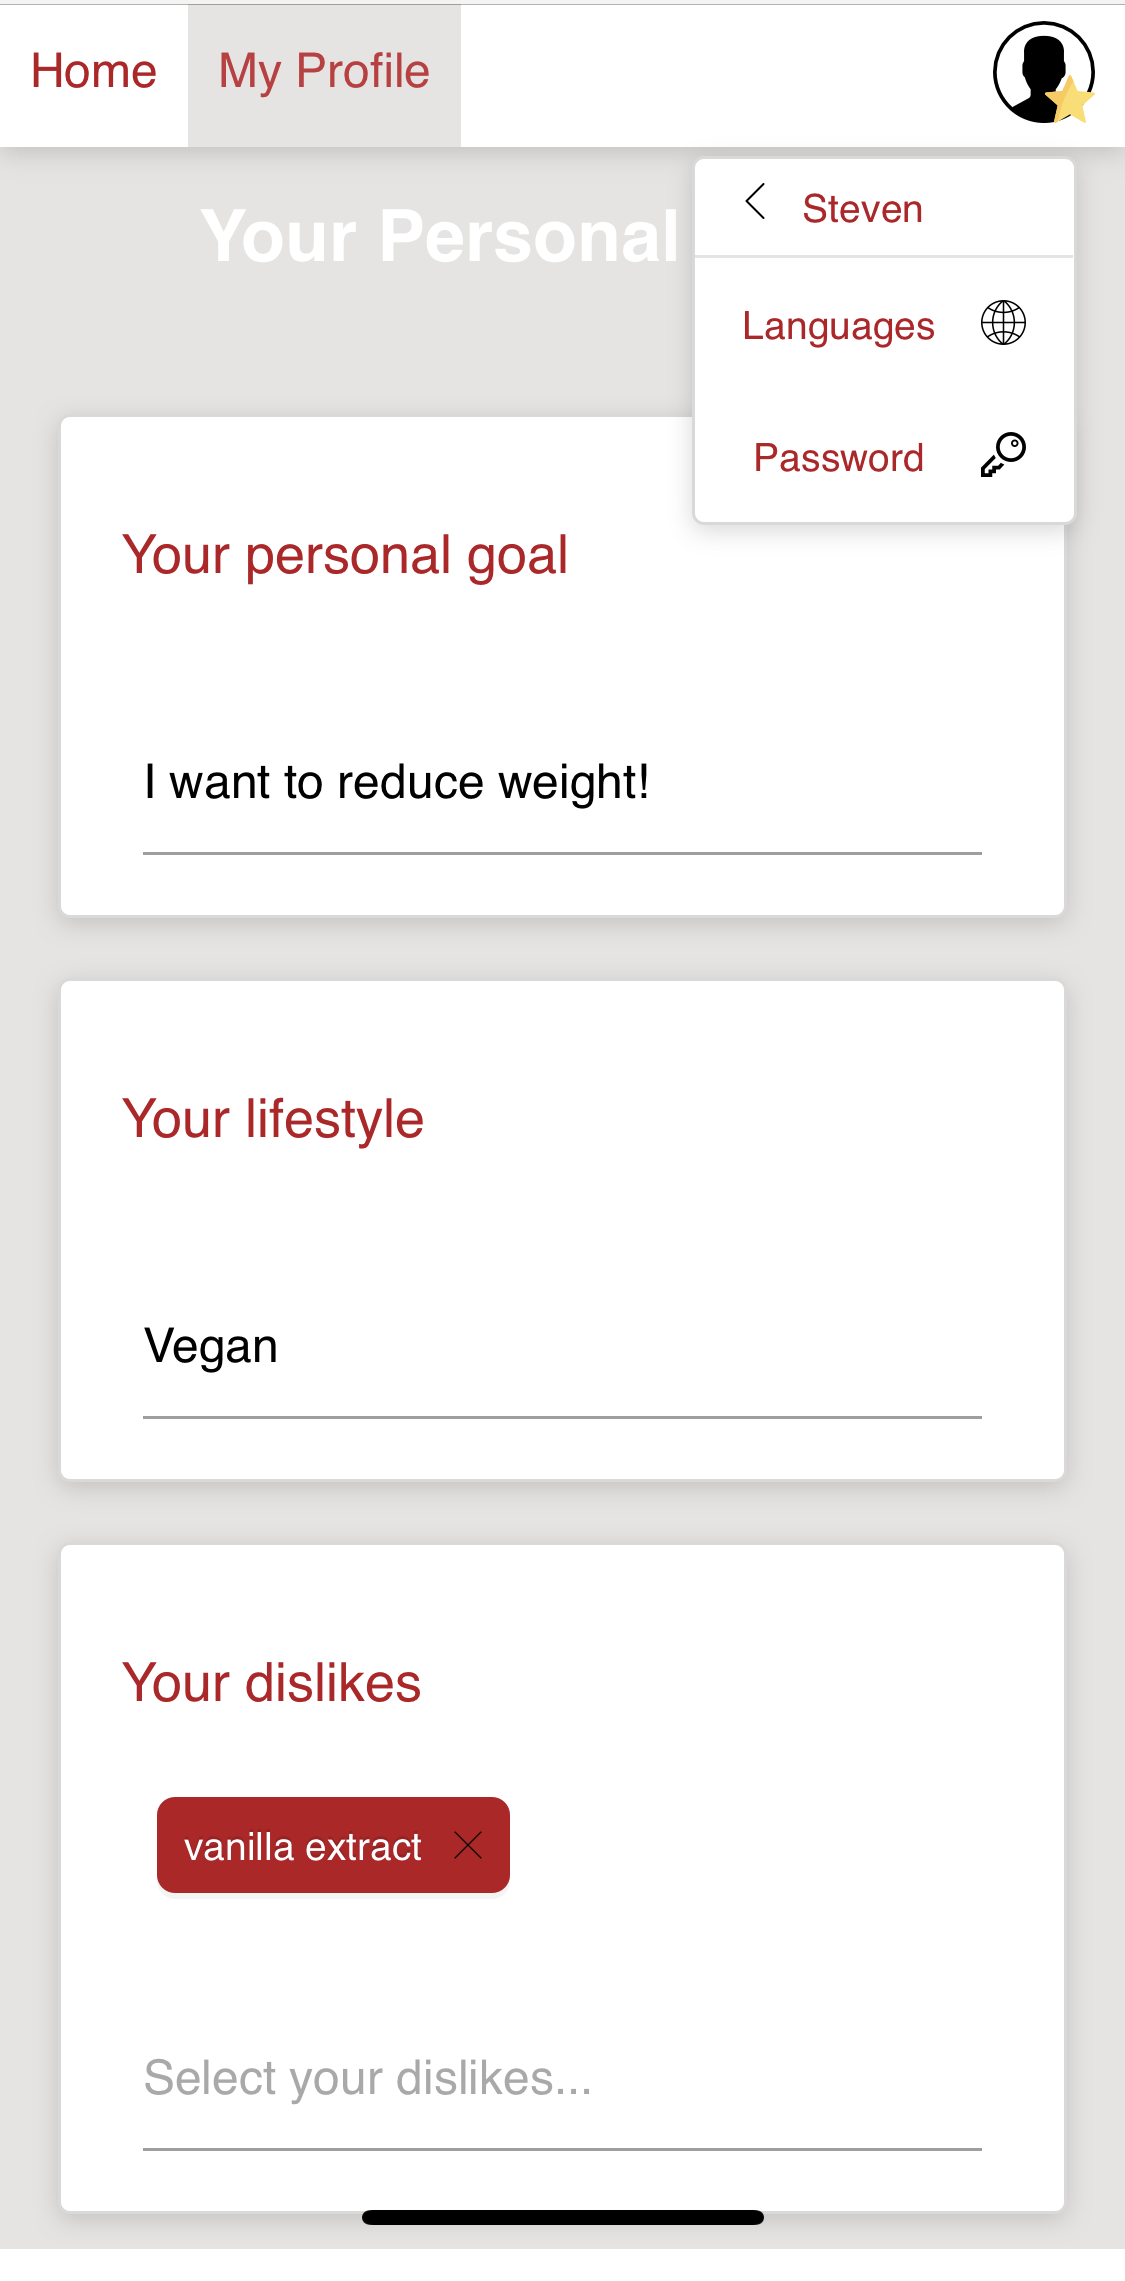
\includegraphics[scale=0.12]{Ressourcen/img/screenshots/iphone1.png}\hfill
	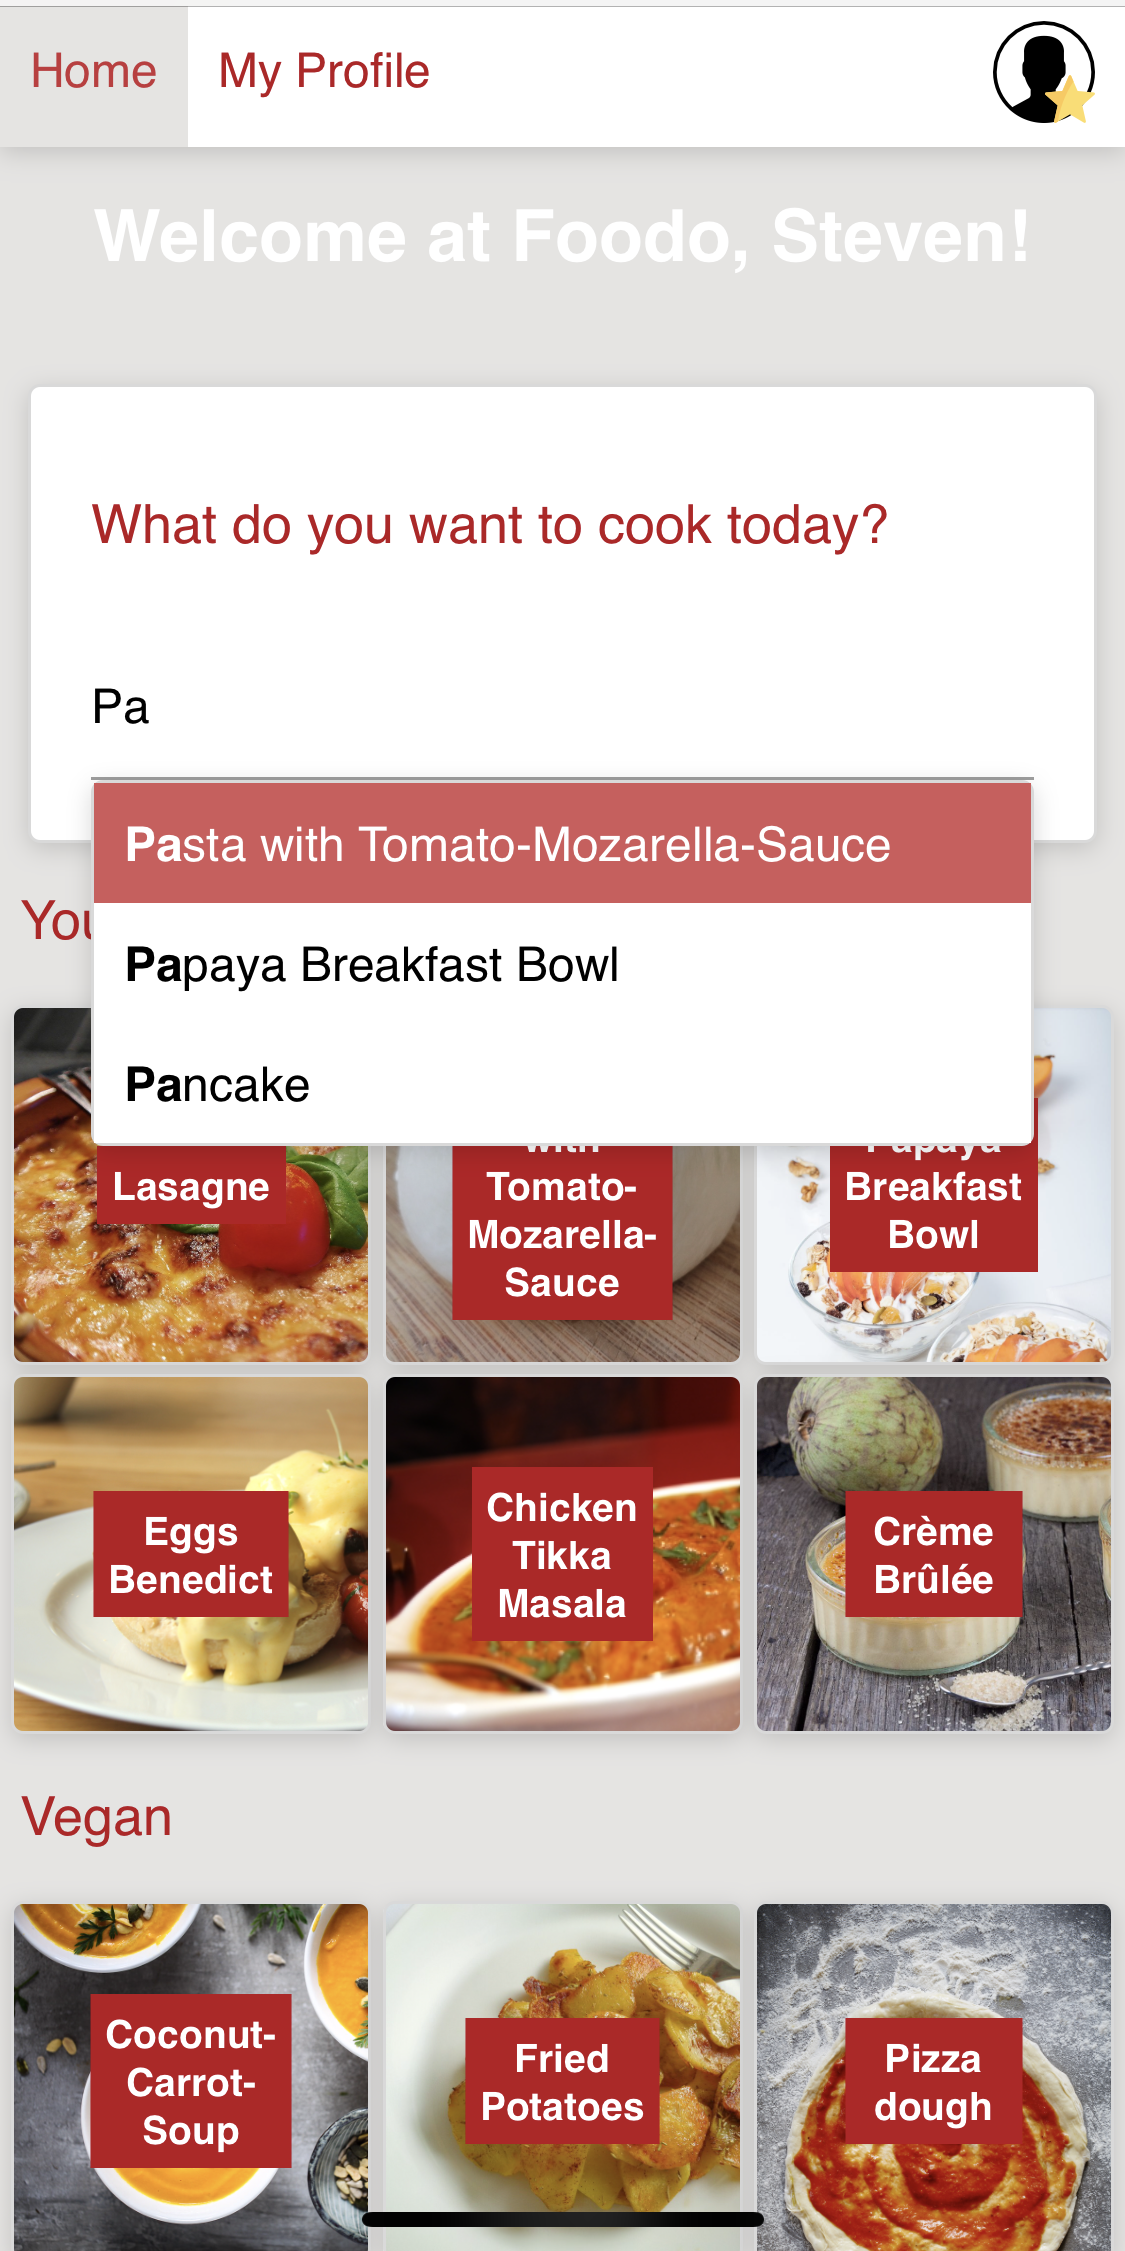
\includegraphics[scale=0.12]{Ressourcen/img/screenshots/iphone2.png}\hfill
		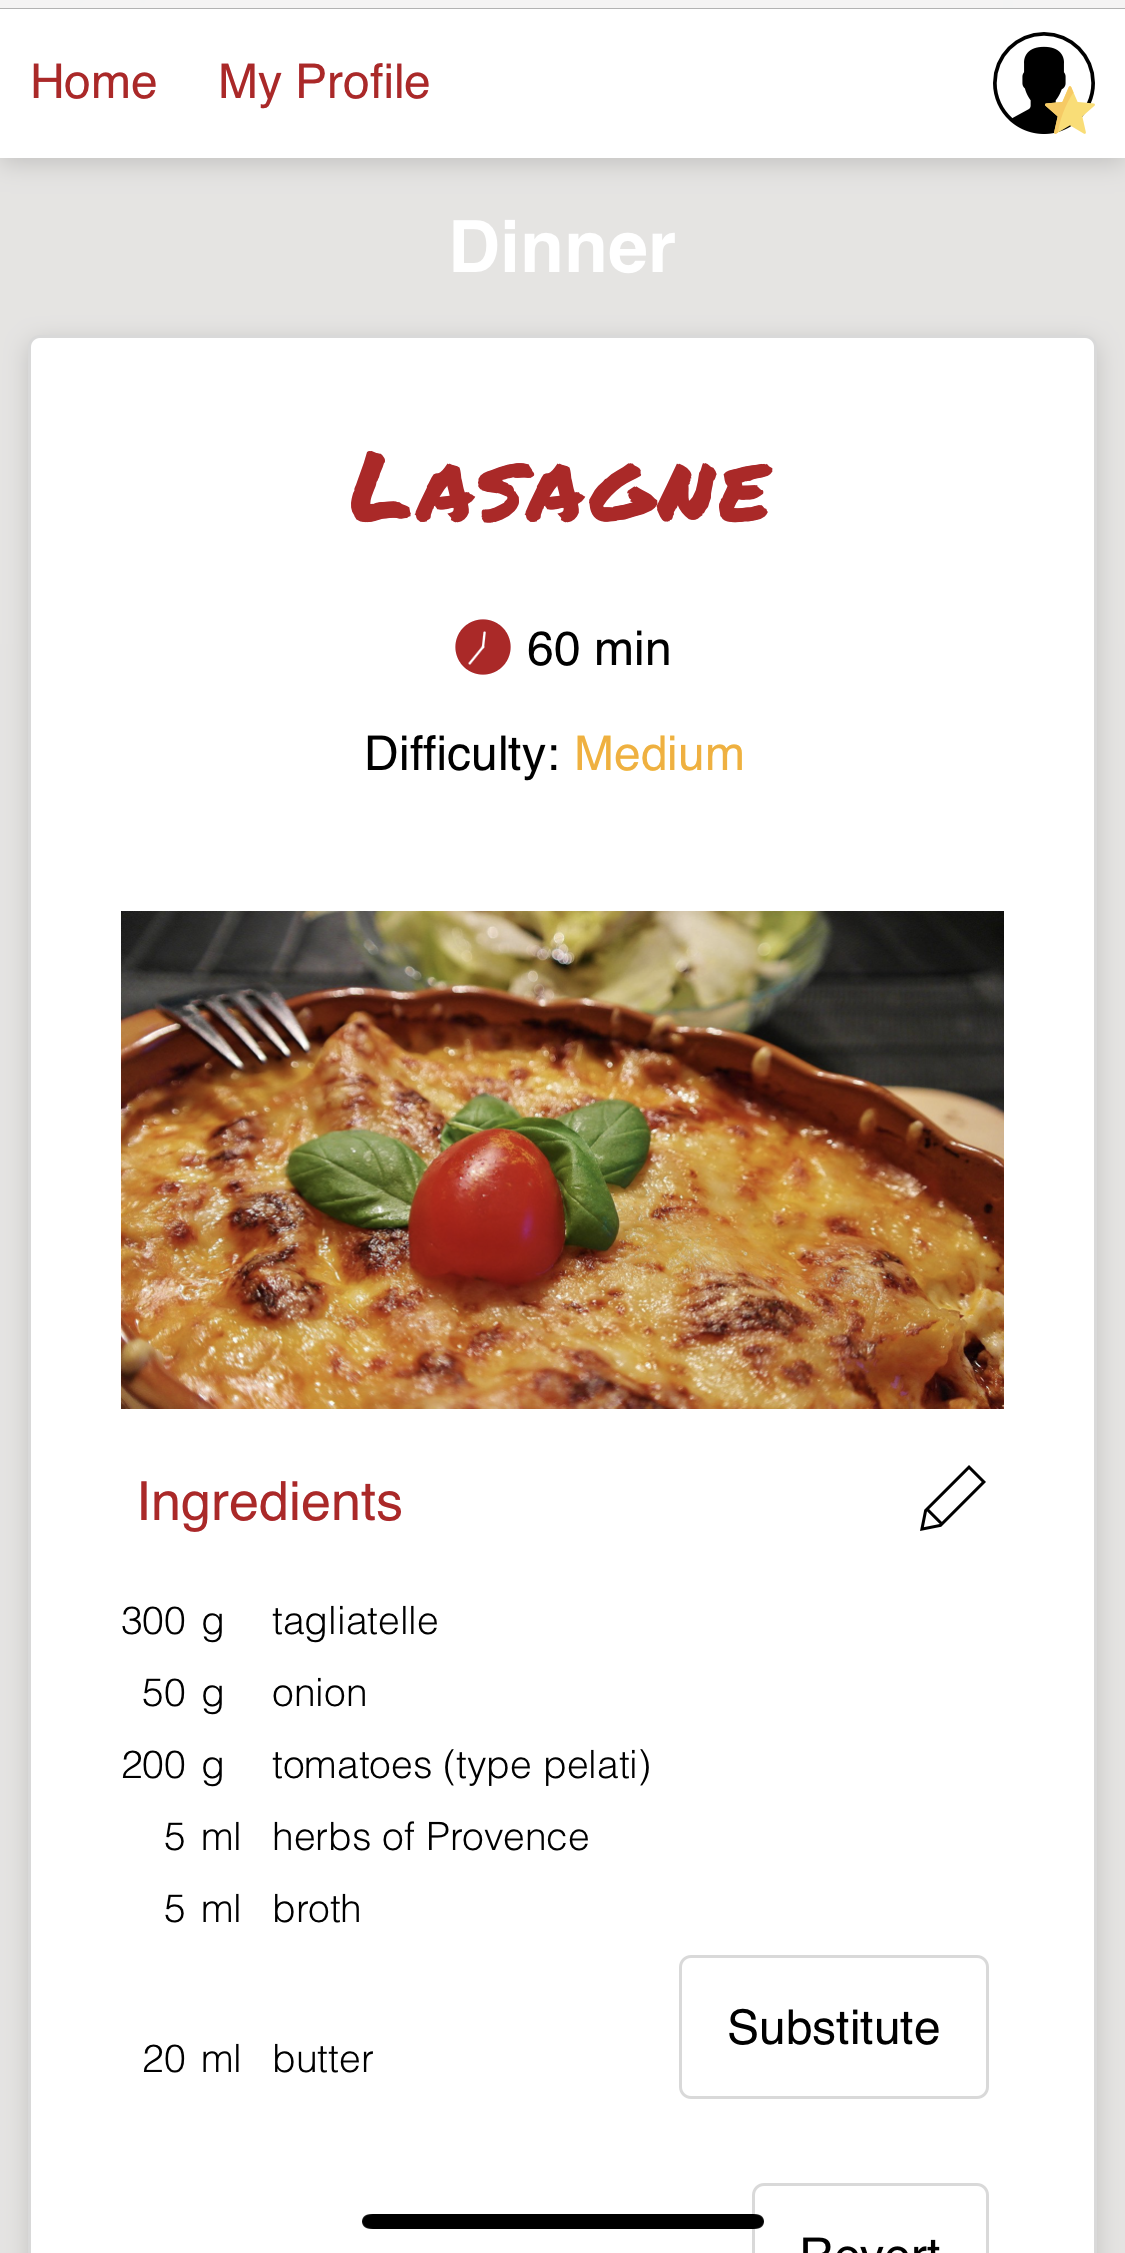
\includegraphics[scale=0.12]{Ressourcen/img/screenshots/iphone3.png}
	\caption{Mobile screenshots}
\end{figure}


